\chapter{Tempering plurality tyranny effects in social choice}
\label{sec:20}


\abstract*{ In a \emph{social choice} context, where decision objectives would match different political parties, Pareto efficient choice recommendations represent in fact \emph{multipartisan} social choices that may judiciously deliver the primary selection in a two stage election system. Our bipolar-valued outranking model is based on approvals-disapprovals of ``\emph{at least as well evaluated as}'' statements. A similar approach is put into practice with approval-disapproval voting systems. When converting such approval-disapproval voting ballots into corresponding performance records, we obtain a $(-1,0,1)$-valued evaluative voting system. We eventually show that in such a approval-disapproval voting system, the winner tends to be among the more or less multipartisan candidates.}

\begin{quotation}\emph{The choice of a voting procedure shapes the democracy in which we live}.\\
    -- \citet*{BAU-2012}.
\end{quotation}
\vspace{1cm}

\abstract{ In a \emph{social choice} context, where decision objectives would match different political parties, Pareto efficient choice recommendations represent in fact \emph{multipartisan} social choices that may judiciously deliver the primary selection in a two stage election system. Our bipolar-valued outranking model is based on approvals-disapprovals of ``\emph{at least as well evaluated as}'' statements. A similar approach is put into practice with approval-disapproval voting systems. When converting such approval-disapproval voting ballots into corresponding performance records, we obtain a $(-1,0,1)$-valued evaluative voting system. We eventually show that in such a approval-disapproval voting system, the winner tends to be among the more or less multipartisan candidates.}

\paragraph{\textbf{Introduction}}

Tempering plurality tyranny effects is, from the seminal work by B. Roy on \citep{ROY-1966}, achieved in the outranking approach by taking into account considerable negative performance differences that may render doubtful otherwise positive ``\emph{at least as well evaluated as}'' situations. In the social choice context of general elections, such a polarisation is not feasible as the genuine uninominal voting ballots do not contain a rich enough preferential information. Yet, when matching decision objectives with political parties, the Pareto efficient outranking situations seen in Section~\ref{sec:19.6}, correspond to multipartisan ``\emph{at least as well approved as}'' situations when pairwisely comparing the eligible candidates. A best choice recommendation based of the corresponding multipartisan strict ``\emph{better approved as}'' situations may, the case given, deliver a convincing primary selection in a two-stage election. 

\section{Two-stage elections with multipartisan primary selection}
\label{sec:20.1}

To compute multipartisan social choices we need to, first, convert a given linear voting profile with pre-election polls into a corresponding performance tableau.

% \subsection{Converting voting profiles into performance tableaux}
% \label{sec:20.1.1}

We shall illustrate this point with a voting profile we discussed already in Chapter~\ref{sec:7}.
\begin{lstlisting}[caption={Example of a 3 parties voting profile},label=list:20.1]
>>> from votingProfiles import RandomLinearVotingProfile
>>> lvp = RandomLinearVotingProfile(numberOfCandidates=15,
...                         numberOfVoters=1000,
...                         WithPolls=True,
...                         partyRepartition=0.5,
...                         other=0.1,
...                         seed=0.9189670954954139)
>>> lvp
  *------- VotingProfile instance description ------*
   Instance class   : RandomLinearVotingProfile
   Instance name    : randLinearProfile
   Candidates       : 15
   Voters           : 1000
   Attributes       : ['name', 'seed', 'candidates',
             'voters', 'WithPolls', 'RandomWeights',
             'sumWeights', 'poll1', 'poll2',
             'other', partyRepartition,
             'linearBallot', 'ballot']
>>> lvp.showRandomPolls()
  Random repartition of voters
   Party_1 supporters : 460 (46.0%)
   Party_2 supporters : 436 (43.6%)
   Other voters       : 104 (10.4%)
  *---------------- random polls ----------------
   Party-1(46.0%) | Party-(43.6%)|  expected  
   ----------------------------------------------
    c06 : 19.91%  | c11 : 22.94%  | c06 : 15.00%
    c07 : 14.27%  | c08 : 15.65%  | c11 : 13.08%
    c03 : 10.02%  | c04 : 15.07%  | c08 : 09.01%
    c13 : 08.39%  | c06 : 13.40%  | c07 : 08.79%
    c15 : 08.39%  | c03 : 06.49%  | c03 : 07.44%
    c11 : 06.70%  | c09 : 05.63%  | c04 : 07.11%
    c01 : 06.17%  | c07 : 05.10%  | c01 : 05.06%
    c12 : 04.81%  | c01 : 05.09%  | c13 : 05.04%
    c08 : 04.75%  | c12 : 03.43%  | c15 : 04.23%
    c10 : 04.66%  | c13 : 02.71%  | c12 : 03.71%
    c14 : 04.42%  | c14 : 02.70%  | c14 : 03.21%
    c05 : 04.01%  | c15 : 00.86%  | c09 : 03.10%
    c09 : 01.40%  | c10 : 00.44%  | c10 : 02.34%
    c04 : 01.18%  | c05 : 00.29%  | c05 : 01.97%
    c02 : 00.90%  | c02 : 00.21%  | c02 : 00.51%
\end{lstlisting}

In this example (see List.~\vref{list:20.1} Lines 20-), we observe 460 Party-1 supporters ($46\%$), 436 Party-2 supporters ($43.6\%$) and 104 other voters ($10.4\%$). Favorite candidates of Party-1 supporters, with more than $10\%$, are \texttt{c06} ($19.91\%$), \texttt{c07} ($14.27\%$) and \texttt{c03} ($10.02\%$). Whereas for Party-2 supporters, favorite candidates are \texttt{c11} ($22.94\%$), followed by \texttt{c08} ($15.65\%$), \texttt{c04} ($15.07\%$) and \texttt{c06} ($13.4\%$).

We can convert this linear voting profile into a \texttt{PerformanceTableau} object where each political party matches a decision objective.
\begin{lstlisting}[caption={Converting a voting profile into a performance tableau},label=list:20.2]
>>> lvp.save2PerfTab('votingPerfTab')
>>> from perfTabs import PerformanceTableau
>>> vpt = PerformanceTableau('votingPerfTab')
>>> vpt
  *------- PerformanceTableau instance description ---*
    Instance class   : PerformanceTableau
    Instance name    : votingPerfTab
    Actions          : 15
    Objectives       : 3
    Criteria         : 1000
    Attributes       : ['name', 'actions', 'objectives',
              'criteria', 'weightPreorder', 'evaluation']
>>> vpt.objectives
  OrderedDict([
    ('party0', {'name': 'other', 'weight': Decimal('104'),
     'criteria': ['v0003', 'v0008', 'v0011', ... ']}),
    ('party1', {'name': 'party 1', 'weight': Decimal('460'),
     'criteria': ['v0002', 'v0006', 'v0007', ...]}),
    ('party2', {'name': 'party 2', 'weight': Decimal('436'),
      'criteria': ['v0001', 'v0004', 'v0005', ... ]})
    ])
\end{lstlisting}

In Listing~\vref{list:20.2} the linear voting profile lvp is first stored in \texttt{PerformanceTableau} format (see Line 1). In Line 3, the PerformanceTableau class reloads this stored performance tableau data. The three parties of the linear voting profile represent three decision objectives and the 1000 voters are distributed as 1000 performance criteria according to the party they support.

% \subsection{Multipartisan primary selection of eligible candidates}
% \label{sec:20.1.2}

In order to operate now a \emph{primary multipartisan selection} of potential election winners, we compute the corresponding unopposed multiobjective outranking digraph (see Sec.~\ref{sec:19.5}).
\begin{lstlisting}[caption={Computing unopposed multiobjective outranking situations},label=list:20.3]
>>> from outrankingDigraphs import \
...       UnOpposedBipolarOutrankingDigraph
>>> uog = UnOpposedBipolarOutrankingDigraph(vpt)
>>> uog
  *------- Object instance description ------*
    Instance class      : UnOpposedBipolarOutrankingDigraph
    Instance name       : unopposed_outrankings
    Actions             : 15
    Criteria            : 1000
    Size                : 34
    Oppositeness (%)    : 67.31
    Determinateness (%) : 57.61
    Valuation domain    : [-1.00;1.00]
    Attributes          : ['name', 'actions', 'valuationdomain',
                           'objectives', 'criteria', 'methodData',
                           'evaluation', 'order', 'runTimes',
                           'relation', 'marginalRelationsRelations',
                           'gamma', 'notGamma']
\end{lstlisting}

From the potential 105 pairwise outranking situations, we keep 34 positively validated outranking situations, leading to a degree of \emph{oppositeness} between political parties of $67.31\%$.

We may visualize the corresponding bipolar-valued relation table by orienting the list of candidates with the help of the initial and terminal prekernels.
\begin{lstlisting}[caption={Computing unopposed multiobjective outranking situations},label=list:20.4]
>>> uog.showPreKernels()
  *--- Computing preKernels ---*
   Dominant preKernels :
    ['c11', 'c06', 'c13', 'c15']
       independence :  0.0
       dominance    :  0.18
       absorbency   :  -0.66
       covering     :  0.43
   Absorbent preKernels :
    ['c02', 'c04', 'c14', 'c03']
       independence :  0.0
       dominance    :  0.0
       absorbency   :  0.37
       covered      :  0.46
>>> orientedCandidatesList = ['c06','c11','c13','c15',\
...         'c01','c05','c07','c08','c09','c10','c12',\
...         'c02','c03','c04','c14']
>>> uog.showHTMLRelationTable(\
...    actionsList=orientedCandidatesList,\
...    tableTitle='Unopposed three-partisan outrankings')
\end{lstlisting}

\begin{figure}[ht]
%\sidecaption
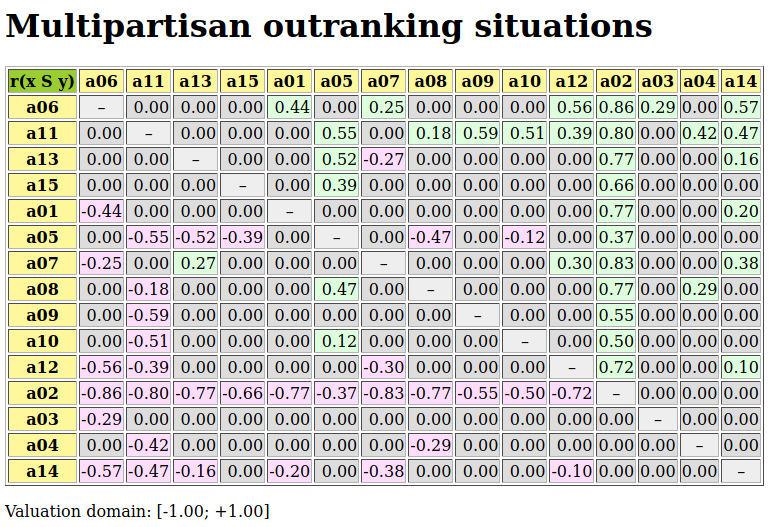
\includegraphics[width=0.9\hsize]{Figures/20-1-unOpposedOutrankings.png}
\caption{Relation table of multipartisan outranking digraph} 
\label{fig:20.1}       % Give a unique label
\end{figure}

In Figure~\vref{fig:20.1}, we may notice that the dominating outranking prekernel \{\texttt{c06}, \texttt{c11}, \texttt{c13}, \texttt{c15}\} gathers in fact a multipartisan selection of potential election winners. It is worthwhile noticing that the majority margins obtained from a linear voting profile do verify the zero-sum rule: $\big(\,r(x \succsim y) \,+\, r(y \succsim x) \;=\; 0.0\,\big)$. To each positive outranking situation corresponds an equivalent negative converse situation and the resulting outranking and strict outranking digraphs are the same.

% \subsection{Secondary election winner determination}
% \label{sec:20.1.3}

When restricting now, in a secondary election stage, the set of eligible candidates to this dominating prekernel, we may compute the actual best social choice.
\begin{lstlisting}[caption={Recommending the secondary election winner},label=list:20.5]
>>> from outrankingDigraphs import BipolarOutrankingDigraph
>>> g2 = BipolarOutrankingDigraph(vpt,\
..          actionsSubset=['c06','c11','c13','c15'])
>>> g2.showRelationTable(ReflexiveTerms=False)
  * ---- Relation Table -----
     r    | 'c06'  'c11'  'c13'  'c15'   
    ------|----------------------------
    'c06' |   -    +0.10  +0.48  +0.52  
    'c11' | -0.10    -    +0.27  +0.29  
    'c13' | -0.48  -0.27    -    +0.19  
    'c15' | -0.52  -0.29  -0.19    -   
    Valuation domain: [-1.0; 1.0]
>>> g2.computeCondorcetWinners()
  ['c06']
>>> g2.computeCopelandRanking()
  ['c06', 'c11', 'c13', 'c15']
\end{lstlisting}

Candidate \texttt{c06} appears clearly to be the winner of this election. Notice by the way that the restricted pairwise outranking relation, shown in Listing~\ref{list:20.5} Lines 7-11, models a linear ordering of the preselected candidates.

We can eventually check the quality of this best choice by noticing that Candidate \texttt{c06} represents indeed the \emph{simple majority}, the \emph{instant-run-off}, the \Borda, as well as the \Condorcet winner of the initially given linear voting profile \texttt{lvp}.
\begin{lstlisting}
>>> lvp.computeSimpleMajorityWinner()
  ['c06']
>>> lvp.computeInstantRunoffWinner()
  ['c06']
>>> lvp.computeBordaWinners()
  ['c06']
>>> from votingProfiles import MajorityMarginsDigraph
>>> cd = MajorityMarginsDigraph(lvp)
>>> cd.computeCondorcetWinners()
  ['c06']
\end{lstlisting}

In our example voting profile here, the multipartisan primary selection stage appears quite effective in reducing the number of eligible candidates to four out of a set of 15 candidates without by the way rejecting the actual winning candidate.

However, in a very \emph{divisive} two major parties system, like in the US, where preferences of the supporters of one major party are opposite to the preferences of the supporters of the other major party, the multipartisan outranking digraph will become nearly indeterminate.

In Listing~\vref{list:20.6} below we generate such a divisive kind of linear voting profile with the help of the \texttt{DivisivePolitics} flag (see Lines 4 and 13-19 in List.~\vref{list:20.6}). When now converting the voting profile into a performance tableau (Lines 20-21), we can compute the corresponding unopposed outranking digraph.
\begin{lstlisting}[caption={A divisive two-party example of a random linear voting profile},label=list:20.6]
>>> from votingProfiles import RandomLinearVotingProfile		     
>>> lvp = RandomLinearVotingProfile(\
...      numberOfCandidates=7,numberOfVoters=500,\
...      WithPolls=True, partyRepartition=0.4,other=0.2,\
...      DivisivePolitics=True, seed=1)
>>> lvp.showRandomPolls()
  Random repartition of voters
   Party-1 supporters : 240 (48.00%)
   Party-2 supporters : 160 (32.00%)
   Other voters       : 100 (20.00%)
  *---------------- random polls -------------
   Party_1(48.0%) | Party_2(32.0%) | expected  
   -------------------------------------------
   c2 : 30.84%    |  c1 : 30.84%   | c2 : 15.56%
   c3 : 23.67%    |  c4 : 23.67%   | c3 : 12.91%
   c7 : 17.29%    |  c6 : 17.29%   | c7 : 11.43%
   c5 : 11.22%    |  c5 : 11.22%   | c1 : 11.00%
   c6 : 09.79%    |  c7 : 09.79%   | c6 : 10.23%
   c4 : 04.83%    |  c3 : 04.83%   | c4 : 09.89%
   c1 : 02.37%    |  c2 : 02.37%   | c5 : 08.98%
>>> lvp.save2PerfTab('divisiveExample')
>>> dvp = PerformanceTableau('divisiveExample')
>>> from outrankingDigraphs import \
...        UnOpposedBipolarOutrankingDigraph
>>> uodg = UnOpposedBipolarOutrankingDigraph(dvp)
>>> uodg
  *------- Object instance description ------*
   Instance class : UnOpposedBipolarOutrankingDigraph
   Instance name  : divisiveExample
   Actions        : 7
   Criteria       : 500
   Size           : 0
   Oppositeness (%)    : 100.00
   Determinateness (%) : 50.00
   Valuation domain    : [-1.00;1.00]
\end{lstlisting}

With an oppositeness degree of $100.0\%$ (see List.~\vref{list:20.6} Lines 31-32), the preferential disagreement between the political parties is complete, and the unopposed outranking digraph \texttt{uodg} becomes completely indeterminate as shown in the relation table below.
\begin{lstlisting}
>>> uodg.showRelationTable(ReflexiveTerms=False)
  * ---- Relation Table -----
   r   | 'c1'   'c2'  'c3'  'c4'  'c5'  'c6'  'c7'   
  -----|------------------------------------------
  'c1' |   -   +0.00 +0.00 +0.00 +0.00 +0.00 +0.00  
  'c2' | +0.00   -   +0.00 +0.00 +0.00 +0.00 +0.00  
  'c3' | +0.00 +0.00   -   +0.00 +0.00 +0.00 +0.00  
  'c4' | +0.00 +0.00 +0.00   -   +0.00 +0.00 +0.00  
  'c5' | +0.00 +0.00 +0.00 +0.00   -   +0.00 +0.00  
  'c6' | +0.00 +0.00 +0.00 +0.00 +0.00   -   +0.00  
  'c7' | +0.00 +0.00 +0.00 +0.00 +0.00 +0.00   -   
  Valuation domain: [-1.0; 1.0]
\end{lstlisting}      

As a consequence, a multipartisan primary selection, computed with a \texttt{show\-Best\-ChoiceRecommendation()} method,  will keep the complete initial set of eligible candidates and, hence, become \emph{ineffective} (see List.~\vref{list:20.7} Line 6).
\begin{lstlisting}[caption={Example of ineffective primary multipartisan selection},label=list:20.7]
>>> uodg.showBestChoiceRecommendation()
  Rubis best choice recommendation(s) (BCR)
   (in decreasing order of determinateness)   
   Credibility domain: [-1.00,1.00]
   === >> ambiguous choice(s)
    choice              : ['c1','c2','c3','c4','c5','c6','c7']
    independence        : 0.00
    dominance           : 1.00
    absorbency          : 1.00
    covered (%)         : 100.00
    determinateness (%) : 50.00
     - most credible action(s) = { }
\end{lstlisting}

With such kind of divisive voting profile, there may indeed not always exist an obvious winner. In Listing~\vref{list:20.8}, we see, for instance, that the simple majority winner is \texttt{c2} (Line 2), whereas the instant-run-off winner is \texttt{c6} (Line 4).
\begin{lstlisting}[caption={Example of non obvious secondary selection},label=list:20.8]
>>> lvp.computeSimpleMajorityWinner()
  ['c2']
>>> lvp.computeInstantRunoffWinner()
  ['c6']
>>> from votingProfiles import MajorityMarginsDigraph
>>> cg = MajorityMarginsDigraph(lvp)
>>> cg.showRelationTable(ReflexiveTerms=False)
  * ---- Relation Table -----
    r()  |  'c1' 'c2' 'c3' 'c4' 'c5' 'c6' 'c7'	  
   ------|------------------------------------
    'c1' |   -   -68  -90  -46  -68  -88  -84	 
    'c2' |  +68   -   -32  +80  +46   -6  -24	 
    'c3' |  +90  +32   -   +58  +46   +4   +8	 
    'c4' |   +4  -80  -58   -   -16  -68  -72	 
    'c5' |  +68  -46  -46  +16	 -   -26  -64	 
    'c6' |  +88   +6   -4  +68	+26   -    -2	 
    'c7' |  +84  +24   -8  +72	+64   +2   - 	 
Valuation domain: [-500;+500]
>>> cg.computeCondorcetWinners()
  ['c3']
>>> lvp.computeBordaWinners()
  ['c3','c7']
>>> cg.computeCopelandRanking()
  ['c3', 'c7', 'c6', 'c2', 'c5', 'c4', 'c1']
\end{lstlisting}

But in our example here, we are lucky. When constructing with the pairwise majority margins digraph (Line 6), a \Condorcet winner, namely \texttt{a3}, becomes apparent (Lines 13,20), which is also one of the two \Borda winners (Line 22). More interesting even is to notice that the apparent majority margins digraph models in fact a linear ranking [\texttt{a3}, \texttt{a7}, \texttt{a6}, \texttt{a2}, \texttt{a5}, \texttt{a4}, \texttt{a1}] of all the eligible candidates, as shown with a \Copeland ranking rule (Line 24).

We may eventually visualize in Figure~\vref{fig:20.2} this linear ranking with a graphviz drawing where we drop all transitive arcs (Line 1) and orient the drawing with \Condorcet winner \texttt{a3} and loser \texttt{a1} (Line 2 below).
\begin{lstlisting}
>>> cg.closeTransitive(Reverse=True)
>>> cg.exportGraphViz('divGraph',\
...            firstChoice=['c3'],lastChoice=['c1'])
  *---- exporting a dot file for GraphViz tools ---------*
   Exporting to divGraph.dot
   dot -Grankdir=BT -Tpng divGraph.dot -o divGraph.png
\end{lstlisting}
\begin{figure}[ht]
\sidecaption[t]
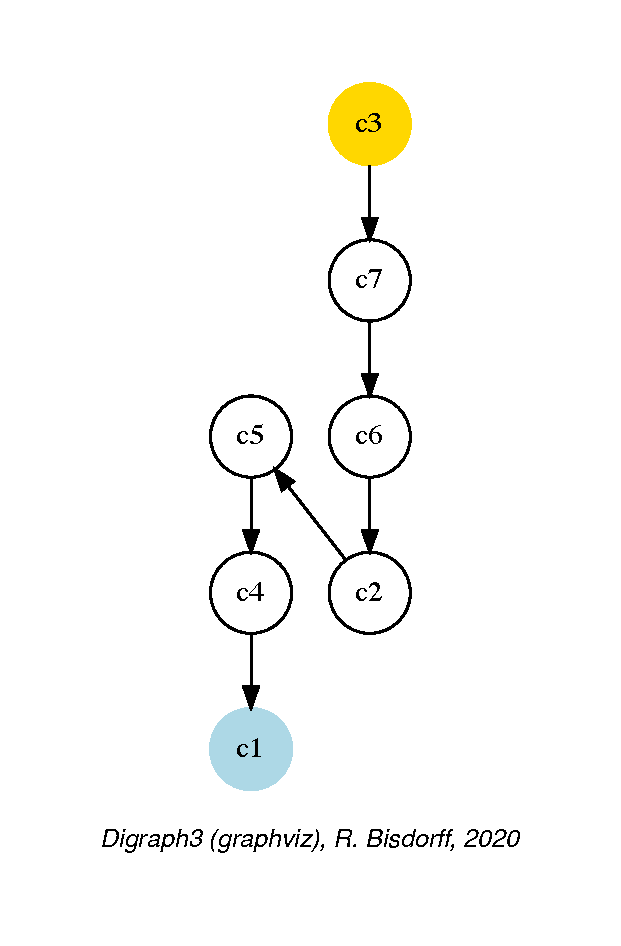
\includegraphics[width=5cm]{Figures/20-2-divGraph.pdf}
\caption{The linear ranking modelled by the majority margins digraph} 
\label{fig:20.2}       % Give a unique label
\end{figure}

\section{Bipolar approval-disapproval voting systems}
\label{sec:20.2}

Traditionally, most of the voting systems in use in the World, do only collect approval votes and abstentions, dismissing potentially strong disapproval opinions, not to be assimilated to voting abstentions. Collecting both explicit approvals ($+1$) and explicit disapprovals ($-1$) essentially enriches the expression of voters' preferences. 

In the \texttt{votingProfiles} module\index{votingProfiles@\texttt{votingProfiles} module} we provide a \texttt{BipolarApprovalVot\-ingProfile} class\index{BipolarApprovalVotingProfile@\texttt{BipolarApprovalVotingProfile} class} for handling voting results where, for each eligible Candidate \texttt{x}, the voters are invited  to \emph{approve} ($+1$), \emph{disapprove} ($-1$), or \emph{ignore} ($0$) the statement that Candidate \texttt{c} should win the election \citep{BAU-2012}.

File \texttt{bpApVotingProfile.py} contains an example of such a approval-disapproval voting profile concerning 100 voters and 15 eligible candidates \footnote{The file \texttt{bpApVotingProfile.py} may be found in the \texttt{examples} directory of the \Digraph resources.}. We may inspect its content as follows.\index{BipolarApprovalVotingProfile@\texttt{BipolarApprovalVotingProfile} class}
\begin{lstlisting}[caption={Bipolar approval vonting profiles},label=list:20.9]
>>> from votingProfiles import \
...                 BipolarApprovalVotingProfile
>>> bavp = BipolarApprovalVotingProfile('bpApVotingProfile')
>>> bavp
  *------- VotingProfile instance description ------*
    Instance class   : BipolarApprovalVotingProfile
    Instance name    : bpApVotingProfile
    Candidates       : 15
    Voters           : 100
    Attributes       : ['name', 'candidates', 'voters',
                 'approvalBallot', 'netApprovalScores',
                 'ballot']
\end{lstlisting}

Beside the \texttt{candidates} and \texttt{voters} attributes, we discover in Listing~\vref{list:20.9} the \texttt{approvalBallot} attribute which gathers approval-disapproval votes. Its content is the following.
\begin{lstlisting}[caption={Inspecting an approval-disapproval ballot},label=list:20.9]
>>> bavp.approvalBallot
  {'v001':
      {'c01': Decimal('0'),
       ...
       'c04': Decimal('1'),
       ...
       'c15': Decimal('0')
      },
   'v002':
       {'c01': Decimal('-1'),
        'c02': Decimal('0'),
        ...
        'c15': Decimal('1')
       },
      ...
   'v100':
     {'c01': Decimal('0'),
      'c02': Decimal('1'),
      ...
      'c15': Decimal('1')
     }
    }
\end{lstlisting}	

Let us denote $A_{\mathtt{v}}$ the set of candidates approved by voter \texttt{v}. In the \texttt{approvalBallot} attribute we hence record in fact the bipolar-valued truth characteristic values $r(\mathtt{c} \in A_{\mathtt{v}})$ of the statements that Candidate \texttt{c} \emph{is approved} by voter \texttt{v}. In Listing~\vref{list:20.9} Line 5, we observe for instance that voter \texttt{v001} positively approves Candidate \texttt{c04}. And, in Line 10, we see that voter \texttt{v002} negatively approves, i.e. positively disapproves Candidate \texttt{c01}.

The \texttt{showApprovalResults()} method\index{showApprovalResults@\texttt{showApprovalResults()}} and the \texttt{showDisapprovalResults()} method\index{showDisapprovalResults@\texttt{showDisapprovalResults()}} show how many approvals, respectively disapprovals, each candidate receives.
\begin{lstlisting}
>>> bavp.showApprovalResults()
    Approval results
     Candidate: 'c12' obtains 34 votes
     Candidate: 'c05' obtains 30 votes
     Candidate: 'c03' obtains 28 votes
     Candidate: 'c14' obtains 27 votes
     Candidate: 'c11' obtains 27 votes
     Candidate: 'c04' obtains 27 votes
     Candidate: 'c01' obtains 27 votes
     Candidate: 'c13' obtains 24 votes
     Candidate: 'c07' obtains 24 votes
     Candidate: 'c15' obtains 23 votes
     Candidate: 'c02' obtains 23 votes
     Candidate: 'c09' obtains 22 votes
     Candidate: 'c08' obtains 22 votes
     Candidate: 'c10' obtains 21 votes
     Candidate: 'c06' obtains 21 votes
    Total approval votes: 380
    Approval proportion: 380/1500 = 0.25
>>> bavp.showDisapprovalResults()
    Disapproval results
     Candidate: 'c12' obtains 16 votes
     Candidate: 'c03' obtains 22 votes
     Candidate: 'c09' obtains 23 votes
     Candidate: 'c04' obtains 24 votes
     Candidate: 'c06' obtains 24 votes
     Candidate: 'c13' obtains 24 votes
     Candidate: 'c11' obtains 25 votes
     Candidate: 'c02' obtains 26 votes
     Candidate: 'c07' obtains 26 votes
     Candidate: 'c08' obtains 26 votes
     Candidate: 'c05' obtains 27 votes
     Candidate: 'c10' obtains 27 votes
     Candidate: 'c14' obtains 27 votes
     Candidate: 'c15' obtains 27 votes
     Candidate: 'c01' obtains 32 votes
    Total disapproval votes: 376
    Disapproval proportion: 376/1500 = 0.25
\end{lstlisting}

In Lines 3 and 22 above, we notice that, of all eligible candidates, it is Candidate \texttt{c12} who receives the highest number of approval votes (34) and the lowest number of disapproval votes (16). Total number of approval, respectively disapproval, votes approaches more or less a proportion of $25\%$ of the $100 \times 15 = 1500$ potential approval votes. About $50\%$ of the latter remain hence ignored. 

When operating now, for each Candidate \texttt{x}, the difference between the number of approval and the number of disapproval votes they receive, we obtain per candidate a corresponding \emph{net approval} score; in fact, the bipolar truth characteristic value of the statement ``\emph{Candidate} \texttt{x} \emph{should win the election}''.
\begin{equation}
r(\text{Candidate x should win the election}) \;=\; \sum_{\mathtt{v}} \big(r(\mathtt{x} \in A_{\mathtt{v}})\big)\;.
\end{equation}

These bipolar characteristic values are stored in the \texttt{netApprovalScores} attribute and may be printed out with the \texttt{showNetApprovalScores()} method\index{showNetApprovalScores@\texttt{showNetApprovalScores()}}:
\begin{lstlisting}
>>> bavp.showNetApprovalScores()
  Net Approval Scores
     Candidate: 'c12' obtains 18 net approvals
     Candidate: 'c03' obtains 6 net approvals
     Candidate: 'c05' obtains 3 net approvals
     Candidate: 'c04' obtains 3 net approvals
     Candidate: 'c11' obtains 2 net approvals
     Candidate: 'c14' obtains 0 net approvals
     Candidate: 'c13' obtains 0 net approvals
     Candidate: 'c09' obtains -1 net approvals
     Candidate: 'c07' obtains -2 net approvals
     Candidate: 'c06' obtains -3 net approvals
     Candidate: 'c02' obtains -3 net approvals
     Candidate: 'c15' obtains -4 net approvals
     Candidate: 'c08' obtains -4 net approvals
     Candidate: 'c01' obtains -5 net approvals
     Candidate: 'c10' obtains -6 net approvals
\end{lstlisting}

We observe in Line 3 above that Candidate \texttt{c12}, with a net approval score of $34 - 16 = 18$, represents indeed the \emph{best approved} candidate for winning the election. With a net approval score of $28-22 = 6$, Candidate \texttt{c03} appears 2nd-best approved. The net approval scores define hence a potentially weak ranking on the set of eligible election candidates, and the winner(s) of the election is(are) determined by the first-ranked candidate(s).

\section{Pairwise comparison of approval-disapproval votes}
\label{sec:20.3}

The approval votes of each voter define now on the set of eligible candidates three ordered categories: his approved ($+1$), his ignored ($0$) and his disapproved ($-1$) ones. Within each of these three categories we consider the voter's actual preferences as \emph{not communicated}, i.e. as missing data. This gives for each voter a partially determined strict order which we find in the \texttt{ballot} attribute.
\begin{lstlisting}
 >>> bavp.ballot['v001']['c12']
    {'c02': Decimal('1'), 'c11': Decimal('1'),
     'c14': Decimal('1'), 'c04': Decimal('0'),
     'c06': Decimal('1'), 'c05': Decimal('1'),
     'c12': Decimal('0'), 'c13': Decimal('0'),
     'c15': Decimal('1'), 'c01': Decimal('1'),
     'c08': Decimal('1'), 'c07': Decimal('1'),
     'c09': Decimal('0'), 'c03': Decimal('1'),
     'c10': Decimal('0')}
\end{lstlisting}

For voter \texttt{v001}, for instance, the best approved Candidate \texttt{c12} is strictly preferred to Candidates: \texttt{c01}, \texttt{c02}, \texttt{c03}, \texttt{c05}, \texttt{c06}, \texttt{c07}, \texttt{c08}, \texttt{c11}, \texttt{c14} and \texttt{c15}. No candidate is preferred to \texttt{c12} and the comparison with \texttt{c04}, \texttt{c09}, \texttt{c10} and \texttt{c13} is not communicated, hence indeterminate. Mind by the way that the reflexive comparison of \texttt{c12} with itself is, as usual, ignored, i.e. indeterminate. Each voter \texttt{v} defines thus a partially determined transitive strict preference relation denoted $\succ_{\mathtt{v}}$ on the eligible candidates.

For each pair of eligible candidates, we aggregate the previous individual voter's preferences into a truth characteristic of the statement: ``Candidate $x$ is \emph{better approved than} Candidate $y$'', denoted $r(x \succ y)$:
\begin{equation}
  r(x \succ y)\;=\; \sum_{\mathtt{v}} \big(\,r(x \succ_{\mathtt{v}} y)\, \big)\;.
\end{equation}  

We say that Candidate $x$ is \emph{better approved than} Candidate $y$ when $r(x \succ y)\;>\;0$, i.e. there is a majority of voters who approve \emph{more} and disapprove \emph{less} $x$ than $y$. Vice-versa, we say that Candidate $x$ is \emph{not} better approved than Candidate $y$ when $r(x \succ y)\;<\;0$, i.e. there is a majority of voters who disapprove more and approve less $x$ than $y$. This computation is achieved with the \texttt{MajorityMarginsDigraph} constructor.
\begin{lstlisting}
>>> from votingProfiles import MajorityMarginsDigraph
>>> m = MajorityMarginsDigraph(bavp)
>>> m
  *------- Digraph instance description ------*
    Instance class      : MajorityMarginsDigraph
    Instance name       : rel_bpApVotingProfile
    Digraph Order       : 15
    Digraph Size        : 97
    Valuation domain    : [-100.00;100.00]
    Determinateness (%) : 52.55
    Attributes          : ['name', 'actions',
               'criteria','ballot',
               'valuationdomain', 'relation',
               'order', 'gamma', 'notGamma']
\end{lstlisting}

The resulting digraph \texttt{m} contains 97 positively validated relations (see Line 8 above) and for all pairs $(x,y)$ of eligible candidates, $r(x \succ y)$ takes value in an valuation range from $-100.00$ (unanimously rejected) to $+100.00$ (unanimously approved).

We may inspect these pairwise $r(x \succ y)$ values in a browser view: 
\begin{lstlisting}
>>> m.showHTMLRelationTable(relationName='r(x > y)')
\end{lstlisting}
\begin{figure}[ht]
%\sidecaption
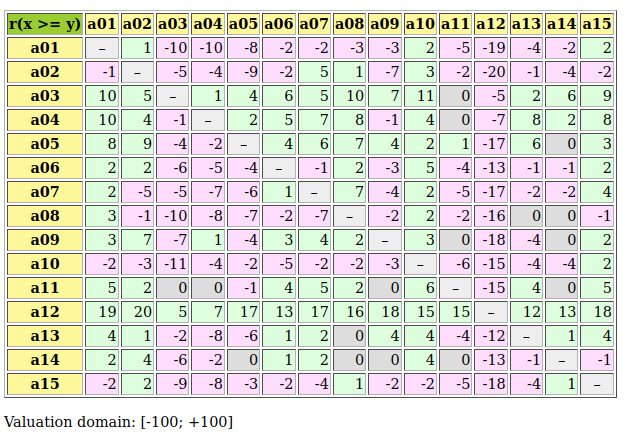
\includegraphics[width=0.8\hsize]{Figures/20-3-majMargAV.png}
\caption{The bipolar-valued pairwise majority margins} 
\label{fig:20.3}       % Give a unique label
\end{figure}

In Figure~\vref{fig:20.3} it gets apparent that Candidate \texttt{c12} is a \Condorcet winner, i.e. the candidate who beats all the other candidates and, with the given voting profile \texttt{gavp}, should without doubt win the election. This strongly confirms the first-ranked result obtained with the previous net approval scoring. 

Let us eventually compute, with the help of the \NetFlows ranking rule\footnote{See Sec.~\ref{sec:8.3}.}, a linear ranking of the 15 eligible candidates and compare the result with the net approval scores ranking.
\begin{lstlisting}[caption={Comparing the net approval and the \NetFlows rankings},label=list:20.10]
>>> from linearOrders import NetFlowsOrder
>>> nf = NetFlowsOrder(m,Comments=True)
>>> print('NetFlows versus Net Approval Ranking')
>>> print('Candidate\tNetFlows score\tNet Approval score')
>>> for item in nf.netFlows:
...     print( '%9s\t  %+.3f\t %+.1f' %\
...	        (item[1], item[0],\
...              bavp.netApprovalScores[item[1]]) ) 
    NetFlows versus Net Approval Ranking
    Candidate	NetFlows score	Net Approval score
      'c12'	  +410.000	 +18.0
      'c03'	  +142.000	  +6.0
      'c04'	   +98.000	  +3.0
      'c05'	   +54.000	  +3.0
      'c11'	   +34.000	  +2.0
      'c09'	   -16.000	  -1.0
      'c14'	   -20.000	  +0.0
      'c13'	   -22.000	  +0.0
      'c06'	   -50.000	  -3.0
      'c07'	   -74.000	  -2.0
      'c02'	   -96.000	  -3.0
      'c08'	   -102.000	  -4.0
      'c15'	   -110.000	  -4.0
      'c10'	   -122.000	  -6.0
      'c01'	   -126.000	  -5.0
\end{lstlisting}

In Listing~\vref{list:20.10} we may notice that the \NetFlows rule delivers a ranking that is very similar to the one previously obtained with the corresponding \emph{Net Approval} scores. Only minor inversions do appear, like in the midfield, where Candidate \texttt{c09} advances before Candidates \texttt{c13} and \texttt{c14} (see Line 16), and \texttt{c06} and \texttt{c07} swap their positions 9 and 10 (see Line 19). The two last-ranked Candidates \texttt{c10} and \texttt{c01} also swap their positions.

This confirms again the pertinence of the net approval scoring approach for finding the winner in an approval-disapproval voting system. Yet, voting by approving ($+1$), disapproving ($-1$) or ignoring ($0$) eligible candidates, may also be seen as a performance evaluation of the eligible candidates on a $\{-1, 0, 1\}$-valued ordinal scale.

\section{Three-valued evaluative voting systems}
\label{sec:20.4}

Following such an epistemic perspective, we may effectively convert the given \texttt{BipolarApprovalVotingProfile} instance into a \texttt{PerformanceTableau} instance, so as to get access to a corresponding outranking decision aiding approach.

Mind that, contrary to the majority margins of the ``\emph{better approved than}'' relation, all voters consider now the approved candidates to be equivalent ($+1$). Same is true for the disapproved ($-1$), respectively the ignored ($0$) candidates. The voter's marginal preferences model this time a complete preorder with three equivalence classes. 

From the saved file \texttt{AVPerfTab.py} (see Line 1 below), we may construct an outranking relation on the eligible candidates with our standard \texttt{BipolarOutran\-kingDigraph} class constructor. The semantics of this outranking relation are the following:
\begin{itemize}[nosep,leftmargin=0.5cm,rightmargin=0.5cm]
\item We say that Candidate $x$ \emph{outranks} Candidate $y$ when there is a majority of voters who consider $x$ \emph{at least as well evaluated as} $y$ (see List.~\vref{list:20.11} Line 3 below);
\item We say that Candidate $x$ is \emph{outranked by} Candidate $y$ when there is a majority of voters who consider $x$ \emph{not at least as well evaluated as} $y$;
\item Otherwise, the outranking situation is indeterminate.
\end{itemize}
\begin{lstlisting}[caption={Computing the outranking digraph},label=list:20.11]
>>> bavp.save2PerfTab(fileName='AVPerfTab',valueDigits=0)
  *--- Saving as performance tableau in AVPerfTab.py ---*
>>> from outrankingDigraphs import\
...                         BipolarOutrankingDigraph
>>> odg = BipolarOutrankingDigraph('AVPerfTab')
>>> odg
  *------- Object instance description ------*
    Instance class       : BipolarOutrankingDigraph
    Instance name        : rel_AVPerfTab
    Actions              : 15
    Criteria             : 100
    Size                 : 210
    Determinateness (%)  : 69.29
    Valuation domain     : [-1.00;1.00]
    Attributes           : ['name', 'actions', 'order,
                       'criteria', 'evaluation', 'NA',
                       'valuationdomain', 'relation',
                       'gamma', 'notGamma', ...]
\end{lstlisting}

The size ($210 = 15 \times 14$) of the resulting outranking digraph \texttt{odg}, shown in Listing~\vref{list:20.11} Line 12 above, reveals that the corresponding ``\emph{at least as good evaluated as}'' relation models actually a trivial \emph{complete} digraph. All candidates appear to be \emph{equally} at least as well evaluated and the strict ``\emph{better evaluated than}'' (codual) outranking digraph becomes in fact empty. The converted performance tableau does apparently not contain sufficiently discriminatory performance evaluations for supporting any strict preference situations.

Yet, we may nevertheless try to apply again the \NetFlows ranking rule to this complete outranking digraph \texttt{odg} and print side by side the corresponding \NetFlows scores and the previous Net Approval scores. 
\begin{lstlisting}[caption={Comparing the \NetFlows and the Net Approval rankings},label=list:20.12]
>>> from linearOrders import NetFlowsOrder
>>> nf = NetFlowsOrder(odg)
>>> print('NetFlows versus Net Approval Ranking')
>>> print('Candidate\tNetFlows Score\tNet Approval Score')
>>> for item in nf.netFlows:
...     print('%9s\t  %+.3f\t %+.0f' %\
...         (item[1],item[0],\
...          bavp.netApprovalScores[item[1]]) )  
    NetFlows versus Net Approval Ranking
    Candidate    NetFlows score	Net Approval score
      c12	  +4.100	    +18
      c03	  +1.420	     +6
      c04	  +0.980	     +3
      c05	  +0.540             +3
      c11	  +0.340	     +2
      c09	  -0.160	     -1
      c14	  -0.200	      0
      c13	  -0.220	      0
      c06	  -0.500	     -3
      c07	  -0.740	     -2
      c02	  -0.960	     -3
      c08	  -1.020	     -4
      c15	  -1.100	     -4
      c10	  -1.220	     -6
      c01	  -1.260	     -5
\end{lstlisting}

Despite its apparent poor strict preference discriminating power, we obtain in Listing~\vref{list:20.12} here \NetFlows scores that are directly proportional (divided by $100$) to the scores obtained with the \emph{better approved than} majority margins digraph \texttt{m} (see List.~\vref{list:20.10}).

Encouraged by this positive result, we may furthermore compute a \Rubis best choice recommendation (see Chap.~\ref{sec:4}).
\begin{lstlisting}[caption={Computing a best social choice recommendation},label=list:20.13]
>>> odg.showBestChoiceRecommendation()
  Rubis best choice recommendation(s) (BCR)
   (in decreasing order of determinateness)   
   Credibility domain: [-1.00,1.00]
  === >> ambiguous first choice(s) 
   * choice        : ['c01','c02','c03','c04','c05',
                      'c06','c07','c08','c09','c10',
                      'c11','c12','c13','c14','c15']
    independence   : 0.06
    dominance      : 1.00
    absorbency     : 1.00
    covering (%)   : 100.00
    determinateness (%) : 61.13
    - most credible action(s) = {
        'c12': 0.44, 'c03': 0.34, 'c04': 0.30,
        'c14': 0.28, 'c13': 0.24, 'c06': 0.24,
        'c11': 0.20, 'c10': 0.20, 'c07': 0.20,
        'c01': 0.20, 'c08': 0.18, 'c05': 0.18,
        'c15': 0.14, 'c09': 0.14, 'c02': 0.06, }
   === >> ambiguous last choice(s)
    * choice        : ['c01','c02','c03','c04','c05',
                      'c06','c07','c08','c09','c10',
                      'c11','c12','c13','c14','c15']
     independence   : 0.06
     dominance      : 1.00
     absorbency     : 1.00
     covered (%)    : 100.00
     determinateness (%) : 63.73
     - most credible action(s) = {
         'c13': 0.36, 'c06': 0.36, 'c15': 0.34,
         'c01': 0.34, 'c08': 0.32, 'c07': 0.30,
         'c02': 0.30, 'c14': 0.28, 'c11': 0.28,
         'c09': 0.28, 'c04': 0.26, 'c10': 0.24,
         'c05': 0.20, 'c03': 0.20, 'c12': 0.06, }
\end{lstlisting}

The strict outranking digraph $(\sim (-odg))$ being actually $empty$, we obtain a unique \emph{ambiguous} --first as well as last-- choice recommendation which trivially retains all fifteen candidates (see List.~\vref{list:20.13} Lines 6-8 above). Yet, the bipolar-valued best choice membership characteristic vector reveals that, among all the fifteen potential winners, it is indeed Candidate \texttt{c12} the most credible one with a $72\%$ majority of voters' support (see Line 15, $(0.44 + 1.0)/2\;=\; 0.72$); followed by Candidate \texttt{c03} ($67\%$) and Candidate \texttt{c04} ($65\%$). Similarly, Candidates \texttt{c13} and \texttt{c06} represent the most credible losers with a $68\%$ majority voters' support (Line 30).

We observe here empirically that \emph{evaluative} voting systems, using three-valued ordinal performance scales, match closely corresponding approval-disapproval voting systems. The latter systems model, however, more faithfully the very preferential information that is expressed with \emph{approved}, \emph{disapproved} and \emph{ignored} statements. The corresponding evaluation on a three-level scale, being value (numbers) based, cannot express the fact that in approval-disapproval voting system there is no preferential information given concerning the pairwise comparison of all approved, respectively disapproved or ignored candidates.

Let us finally illustrate how approval-disapproval voting systems may favour multipartisan supported candidates. We shall therefore compare \emph{approval-disapproval} versus \emph{uninominal plurality} election results when considering a highly divisive and partisan political context.
 
\section{Favouring multipartisan candidates}
\label{sec:20.5}

In modern democracy, politics  are largely structured by political parties and activists. Let us so consider an approval-disapproval voting profile \texttt{dvp} where the random voter behaviour is simulated from two pre-electoral polls concerning a political scene with essentially two major highly competing parties, like the one existing in the US.
\begin{lstlisting}[caption={A random approval-disapproval voting profile in a divisive political context},label=list:20.14]
>>> dvp = RandomBipolarApprovalVotingProfile(\
...                numberOfCandidates=15,\
...                numberOfVoters=100,
...                approvalProbability=0.25,
...                disapprovalProbability=0.25,
...                WithPolls=True,
...                partyRepartition=0.5,
...                other=0.05,
...                DivisivePolitics=True,
...                seed=200)
>>> dvp.showRandomPolls()
  Random repartition of voters
  Party-1 supporters : 45 (45.00%)
  Party-2 supporters : 49 (49.00%)
  Other voters       : 6 (06.00%)
  *---------------- random polls -----------------
  Party-1(45.0%) | Party-2(49.0%) |   expected  
  ------------------------------------------------
  'c05' : 24.10% | 'c07' : 24.10% | 'c07' : 11.87%
  'c14' : 23.48% | 'c10' : 23.48% | 'c10' : 11.60%
  'c03' : 15.13% | 'c01' : 15.13% | 'c05' : 10.91%
  'c12' : 07.55% | 'c04' : 07.55% | 'c14' : 10.67%
  'c08' : 07.11% | 'c09' : 07.11% | 'c01' : 07.67%
  'c15' : 04.37% | 'c13' : 04.37% | 'c03' : 07.09%
  'c11' : 03.99% | 'c02' : 03.99% | 'c04' : 04.55%
  'c06' : 03.80% | 'c06' : 03.80% | 'c09' : 04.49%
  'c02' : 02.79% | 'c11' : 02.79% | 'c12' : 04.32%
  'c13' : 02.63% | 'c15' : 02.63% | 'c08' : 04.30%
  'c09' : 02.24% | 'c08' : 02.24% | 'c06' : 03.57%
  'c04' : 01.89% | 'c12' : 01.89% | 'c13' : 03.32%
  'c01' : 00.57% | 'c03' : 00.57% | 'c15' : 03.25%
  'c10' : 00.20% | 'c14' : 00.20% | 'c02' : 03.21%
  'c07' : 00.14% | 'c05' : 00.14% | 'c11' : 03.16%
\end{lstlisting}   

In Listing~\vref{list:20.14}, the divisive political situation is reflected by the fact that Party-1 and Party-2 supporters show strict opposite preferences. The leading candidates of Party-1 (\texttt{c05} and \texttt{c14}) are last choices for Party-2 supporters and, Candidates \texttt{c07} and \texttt{c10}, leading candidates for Party-2 supporters, are similarly the least choices for Party-1 supporters.

No clear winner may be guessed from these pre-election polls. As Party-2 shows however slightly more supporters than Party-1, the expected winner in an uninominal plurality or instant-run-off voting system will be Candidate \texttt{c07}, i,e, the leading candidate of majority Party-2 (see below).
\begin{lstlisting}
>>> dvp.computeSimpleMajorityWinner()
  ['c07']
>>> dvp.computeInstantRunoffWinner()
  ['c07']
\end{lstlisting}

Now, in a corresponding approval-disapproval voting system, Party-1 supporters will usually approve their leading candidates and disapprove the leading candidates of Party-2. Vice versa, Party-2 supporters will usually approve their leading candidates and disapprove the leading candidates of Party-1. Let us consult the resulting approval votes per candidate.
\begin{lstlisting}
>>> dvp.showApprovalResults()
     Candidate: 'c07' obtains 30 votes
     Candidate: 'c10' obtains 28 votes
     Candidate: 'c05' obtains 28 votes
     Candidate: 'c01' obtains 28 votes
     Candidate: 'c03' obtains 26 votes
     Candidate: 'c02' obtains 26 votes
     Candidate: 'c12' obtains 25 votes
     Candidate: 'c14' obtains 24 votes
     Candidate: 'c13' obtains 24 votes
     Candidate: 'c09' obtains 21 votes
     Candidate: 'c04' obtains 21 votes
     Candidate: 'c08' obtains 19 votes
     Candidate: 'c06' obtains 17 votes
     Candidate: 'c15' obtains 15 votes
     Candidate: 'c11' obtains 12 votes
    Total approval votes: 344
    Approval proportion: 344/1500 = 0.23
\end{lstlisting}

When considering only the approval votes, we find confirmed above that the leading candidate of Party-2 obtains in this simulation a plurality of approval votes. In uninominal plurality or instant-runoff voting systems, this candidate wins hence the election, quite to the despair of Party-1 supporters. As a foreseeable consequence, this election result will be more or less aggressively contested which leads to a loss of popular trust in democratic elections and institutions.

If we look however on the corresponding disapprovals, we discover that, not surprisingly, the leading candidates of both parties collect by far the highest number of disapproval votes. 
\begin{lstlisting}
>>> dvp.showDisapprovalResults()
     Candidate: 'c02' obtains 14 votes
     Candidate: 'c04' obtains 14 votes
     Candidate: 'c13' obtains 14 votes
     Candidate: 'c06' obtains 15 votes
     Candidate: 'c09' obtains 15 votes
     Candidate: 'c08' obtains 16 votes
     Candidate: 'c11' obtains 16 votes
     Candidate: 'c15' obtains 18 votes
     Candidate: 'c12' obtains 20 votes
     Candidate: 'c01' obtains 29 votes
     Candidate: 'c03' obtains 30 votes
     Candidate: 'c10' obtains 37 votes
     Candidate: 'c07' obtains 44 votes
     Candidate: 'c14' obtains 45 votes
     Candidate: 'c05' obtains 49 votes
    Total disapproval votes: 376
    Disapproval proportion: 376/1500 = 0.25
\end{lstlisting}

Balancing now approval against disapproval votes will favour the moderate, bipartisan supported, candidates.
\begin{lstlisting}
>>> dvp.showNetApprovalScores()
    Net Approval Scores
     Candidate: 'c02' obtains 12 net approvals
     Candidate: 'c13' obtains 10 net approvals
     Candidate: 'c04' obtains 7 net approvals
     Candidate: 'c09' obtains 6 net approvals
     Candidate: 'c12' obtains 5 net approvals
     Candidate: 'c08' obtains 3 net approvals
     Candidate: 'c06' obtains 2 net approvals
     Candidate: 'c01' obtains -1 net approvals
     Candidate: 'c15' obtains -3 net approvals
     Candidate: 'c11' obtains -4 net approvals
     Candidate: 'c03' obtains -4 net approvals
     Candidate: 'c10' obtains -9 net approvals
     Candidate: 'c07' obtains -14 net approvals
     Candidate: 'c14' obtains -21 net approvals
     Candidate: 'c05' obtains -21 net approvals
\end{lstlisting}

Candidate \texttt{c02}, appearing in the pre-electoral polls in the midfield (in position 7 for Party-2 and in position 9 for Party-1 supporters, see List.\vref{list:20.14}), shows indeed the highest net approval score. Second highest net approval score obtains Candidate \texttt{c13}, in  position 6 for Party-2 and in position 10 for Party-1 supporters.

Figure~\vref{fig:20.4}, showing the \NetFlows ranked relation table of the ``\emph{better approved than}'' majority margins digraph, confirms below this net approval scoring result.
\begin{lstlisting}
>>> m = MajorityMarginsDigraph(dvp)
>>> m.showHTMLRelationTable(\
...      actionsList=m.computeNetFlowsRanking(),
...      relationName='r(x > y)')
\end{lstlisting}	   
\begin{figure}[ht]
%\sidecaption
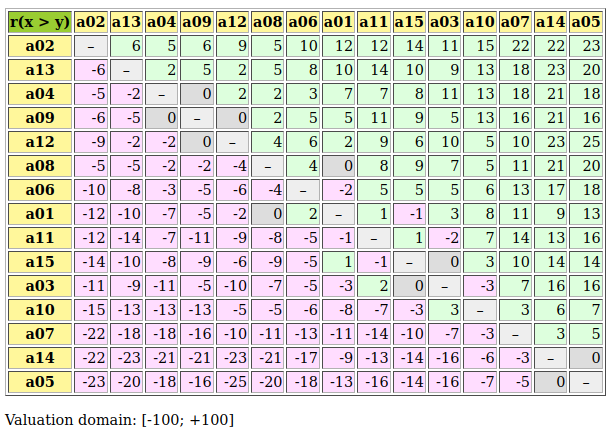
\includegraphics[width=0.8\hsize]{Figures/20-4-majMargDAV.png}
\caption{The pairwise \emph{better approved than} majority margins} 
\label{fig:20.4}       % Give a unique label
\end{figure}

Candidate \texttt{c02} appears indeed \emph{better approved than} any other candidate (\Condorcet winner); and, the leading Candidates of Party-1, \texttt{c05} and \texttt{c14}, are \emph{less approved than} any other candidates (weak \Condorcet losers).
\begin{lstlisting}
>>> m.computeCondorcetWinners()
  ['c02']
>>> m.computeWeakCondorcetLosers()
  ['c05','c14']
\end{lstlisting}

We see this result furthermore confirmed when computing the corresponding first, respectively last choice recommendation.    
\begin{lstlisting}
>>> m.showBestChoiceRecommendation()
  Rubis best choice recommendation(s) (BCR)
   (in decreasing order of determinateness)   
   Credibility domain: [-100.00,100.00]
   === >> potential first choice(s)
    * choice              : ['c02']
      independence        : 100.00
      dominance           : 5.00
      absorbency          : -23.00
      covering (%)        : 100.00
      determinateness (%) : 52.50
      - most credible action(s) = { 'c02': 5.00, }
   === >> potential last choice(s) 
    * choice              : ['c05', 'c14']
      independence        : 0.00
      dominance           : -23.00
      absorbency          : 5.00
      covered (%)         : 100.00
      determinateness (%) : 50.00
      - most credible action(s) = { }
\end{lstlisting}

Candidate \texttt{c02}, being actually a \Condorcet winner, gives an initial prekernel of digraph $m$, whereas Party-1 leading Candidates \texttt{c05} and \texttt{c14}, both being weak \Condorcet losers, give together a terminal prekernel. They hence represent our \emph{first choice}, respectively, \emph{last choice} recommendations for winning this simulated election.

Let us conclude by predicting that, for leading political candidates in an aggressively divisive political context, the perspective to easily fail election withan approval-disapproval voting system, might or will induce a change in the usual way of running electoral campaigns. Political parties and politicians, who avoid aggressive competitive propaganda and instead propose multipartisan collaborative social choices, will be rewarded with better election results than any kind of extremism. It could mean the end of sterile political obstructions and war like electoral battles. \emph{Let's do it !}.

It is worthwhile noticing again the essential structural and computational role, the ignored value is playing in approval-disapproval voting systems. This epistemic and logical \emph{neutral} term is needed indeed for handling in a consistent and efficient manner \emph{not communicated votes} and/or \emph{indeterminate} preferential statements.
 
%%%%%%% The chapter bibliography
%\normallatexbib
%\clearpage
%\phantomsection
%\addcontentsline{toc}{section}{Chapter Bibliography}
\chapter{Tempering plurality tyranny effects in social choice}
\label{sec:20}


\abstract*{ In a \emph{social choice} context, where decision objectives would match different political parties, Pareto efficient choice recommendations represent in fact \emph{multipartisan} social choices that may judiciously deliver the primary selection in a two stage election system. Our bipolar-valued outranking model is based on approvals-disapprovals of ``\emph{at least as well evaluated as}'' statements. A similar approach is put into practice with approval-disapproval voting systems. When converting such approval-disapproval voting ballots into corresponding performance records, we obtain a $(-1,0,1)$-valued evaluative voting system. We eventually show that in such a approval-disapproval voting system, the winner tends to be among the more or less multipartisan candidates.}

\begin{quotation}\emph{The choice of a voting procedure shapes the democracy in which we live}.\\
    -- \citet*{BAU-2012}.
\end{quotation}
\vspace{1cm}

\abstract{ In a \emph{social choice} context, where decision objectives would match different political parties, Pareto efficient choice recommendations represent in fact \emph{multipartisan} social choices that may judiciously deliver the primary selection in a two stage election system. Our bipolar-valued outranking model is based on approvals-disapprovals of ``\emph{at least as well evaluated as}'' statements. A similar approach is put into practice with approval-disapproval voting systems. When converting such approval-disapproval voting ballots into corresponding performance records, we obtain a $(-1,0,1)$-valued evaluative voting system. We eventually show that in such a approval-disapproval voting system, the winner tends to be among the more or less multipartisan candidates.}

\paragraph{\textbf{Introduction}}

From the seminal work by \emph{Bernard Roy}\index{Roy@\textsl{B. Roy}} on, tempering plurality tyranny effects is achieved in the outranking approach by taking into account considerable negative performance differences that render doubtful otherwise positive ``\emph{at least as well evaluated as}'' situations \citep*{ROY-1966}. In the social choice context of general elections, such a polarisation is not feasible as the genuine uninominal voting ballots do not contain a rich enough preferential information. Yet, when matching decision objectives with political parties, the Pareto efficient outranking situations seen in Sect.~\ref{sec:19.6}, correspond to multipartisan ``\emph{at least as well approved as}'' situations when pairwisely comparing the eligible candidates. A best choice recommendation based of the corresponding multipartisan strict ``\emph{better approved as}'' situations may, the case given, deliver a convincing primary selection in a two-stage election. 

\section{Two-stage elections with multipartisan primary selection}
\label{sec:20.1}

To compute multipartisan social choices we need to, first, convert a given linear voting profile with pre-election polls into a corresponding performance tableau. We shall illustrate this point with a voting profile we discussed already in Chap.~\ref{sec:7}.
\begin{lstlisting}[caption={Example of a 3 parties voting profile},label=list:20.1]
>>> from votingProfiles import RandomLinearVotingProfile
>>> lvp = RandomLinearVotingProfile(numberOfCandidates=15,
...                         numberOfVoters=1000,
...                         WithPolls=True,
...                         partyRepartition=0.5,
...                         other=0.1,
...                         seed=0.9189670954954139)
>>> lvp
  *------- VotingProfile instance description ------*
   Instance class   : RandomLinearVotingProfile
   Instance name    : randLinearProfile
   Candidates       : 15
   Voters           : 1000
   Attributes       : ['name', 'seed', 'candidates',
             'voters', 'WithPolls', 'RandomWeights',
             'sumWeights', 'poll1', 'poll2',
             'other', partyRepartition,
             'linearBallot', 'ballot']
>>> lvp.showRandomPolls() §\label{line:20.1.20}§
  Random repartition of voters
   Party_1 supporters : 460 (46.0%)
   Party_2 supporters : 436 (43.6%)
   Other voters       : 104 (10.4%)
  *---------------- random polls ----------------
   Party-1(46.0%) | Party-(43.6%)|  expected  
   ----------------------------------------------
    c06 : 19.91%  | c11 : 22.94%  | c06 : 15.00%
    c07 : 14.27%  | c08 : 15.65%  | c11 : 13.08%
    c03 : 10.02%  | c04 : 15.07%  | c08 : 09.01%
    c13 : 08.39%  | c06 : 13.40%  | c07 : 08.79%
    c15 : 08.39%  | c03 : 06.49%  | c03 : 07.44%
    c11 : 06.70%  | c09 : 05.63%  | c04 : 07.11%
    c01 : 06.17%  | c07 : 05.10%  | c01 : 05.06%
    c12 : 04.81%  | c01 : 05.09%  | c13 : 05.04%
    c08 : 04.75%  | c12 : 03.43%  | c15 : 04.23%
    c10 : 04.66%  | c13 : 02.71%  | c12 : 03.71%
    c14 : 04.42%  | c14 : 02.70%  | c14 : 03.21%
    c05 : 04.01%  | c15 : 00.86%  | c09 : 03.10%
    c09 : 01.40%  | c10 : 00.44%  | c10 : 02.34%
    c04 : 01.18%  | c05 : 00.29%  | c05 : 01.97%
    c02 : 00.90%  | c02 : 00.21%  | c02 : 00.51% §\label{line:20.1.end}§
\end{lstlisting}

In this example (see List.~\vref{list:20.1} Lines~\ref{line:20.1.20}-\ref{line:20.1.end}), we observe 460 Party-1 supporters ($46\%$), 436 Party-2 supporters ($43.6\%$) and 104 other voters ($10.4\%$). Favorite candidates of Party-1 supporters, with more than $10\%$, are \texttt{c06} ($19.91\%$), \texttt{c07} ($14.27\%$) and \texttt{c03} ($10.02\%$). Whereas for Party-2 supporters, favorite candidates are \texttt{c11} ($22.94\%$), followed by \texttt{c08} ($15.65\%$), \texttt{c04} ($15.07\%$) and \texttt{c06} ($13.4\%$).

We can convert this linear voting profile into a \texttt{PerformanceTableau} object where each political party matches a decision objective.
\begin{lstlisting}[caption={Converting a voting profile into a performance tableau},label=list:20.2]
>>> lvp.save2PerfTab('votingPerfTab')§\label{line:20.2.1}§
>>> from perfTabs import PerformanceTableau
>>> vpt = PerformanceTableau('votingPerfTab')§\label{line:20.2.3}§
>>> vpt
  *------- PerformanceTableau instance description ---*
    Instance class   : PerformanceTableau
    Instance name    : votingPerfTab
    Actions          : 15
    Objectives       : 3
    Criteria         : 1000
    Attributes       : ['name', 'actions', 'objectives',
              'criteria', 'weightPreorder', 'evaluation']
>>> vpt.objectives
  OrderedDict([
    ('party0', {'name': 'other', 'weight': Decimal('104'),
     'criteria': ['v0003', 'v0008', 'v0011', ... ']}),
    ('party1', {'name': 'party 1', 'weight': Decimal('460'),
     'criteria': ['v0002', 'v0006', 'v0007', ...]}),
    ('party2', {'name': 'party 2', 'weight': Decimal('436'),
      'criteria': ['v0001', 'v0004', 'v0005', ... ]})
    ])
\end{lstlisting}

In Listing~\vref{list:20.2} the linear voting profile lvp is first stored in \texttt{Performance\-Tableau} format (see Line~\ref{line:20.2.1}). In Line~\ref{line:20.2.3}, the PerformanceTableau class reloads this stored performance tableau data. The three parties of the linear voting profile represent three decision objectives and the 1000 voters are distributed as 1000 performance criteria according to the party they support.

In order to operate now a \emph{primary multipartisan selection} of potential election winners, we compute the corresponding unopposed multiobjective outranking digraph (see Sect.~\ref{sec:19.5}).
\begin{lstlisting}[caption={Computing unopposed multiobjective outranking situations},label=list:20.3]
>>> from outrankingDigraphs import \
...       UnOpposedBipolarOutrankingDigraph
>>> uog = UnOpposedBipolarOutrankingDigraph(vpt)
>>> uog
  *------- Object instance description ------*
    Instance class      : UnOpposedBipolarOutrankingDigraph
    Instance name       : unopposed_outrankings
    Actions             : 15
    Criteria            : 1000
    Size                : 34
    Oppositeness (%)    : 67.31 §\label{line:20.3.opp}§
    Determinateness (%) : 57.61
    Valuation domain    : [-1.00;1.00]
    Attributes          : ['name', 'actions', 'valuationdomain',
                           'objectives', 'criteria', 'methodData',
                           'evaluation', 'order', 'runTimes',
                           'relation', 'marginalRelationsRelations',
                           'gamma', 'notGamma']
\end{lstlisting}

From the potential 105 pairwise outranking situations, we keep 34 positively validated outranking situations, leading to a degree of \emph{oppositeness} between political parties of $67.31\%$ (see List.~\ref{list:20.3} Line~\ref{line:20.3.opp}).

The corresponding bipolar-valued relation table can be shown by orienting the list of candidates with the help of the initial and terminal prekernels.\index{showPreKernels@\texttt{showPreKernels()}}
\begin{lstlisting}[caption={Computing unopposed multiobjective outranking situations},label=list:20.4]
>>> uog.showPreKernels()
  *--- Computing preKernels ---*
   Dominant preKernels :
    ['c11', 'c06', 'c13', 'c15']
       independence :  0.0
       dominance    :  0.18
       absorbency   :  -0.66
       covering     :  0.43
   Absorbent preKernels :
    ['c02', 'c04', 'c14', 'c03']
       independence :  0.0
       dominance    :  0.0
       absorbency   :  0.37
       covered      :  0.46
>>> orientedCandidatesList = ['c06','c11','c13','c15',\
...         'c01','c05','c07','c08','c09','c10','c12',\
...         'c02','c03','c04','c14']
>>> uog.showHTMLRelationTable(\
...    actionsList=orientedCandidatesList,\
...    tableTitle='Unopposed three-partisan outrankings')
\end{lstlisting}

\begin{figure}[ht]
%\sidecaption
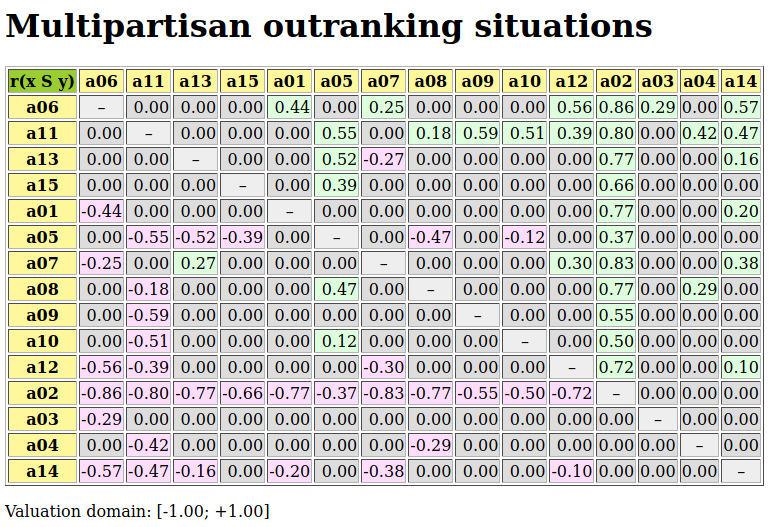
\includegraphics[width=0.9\hsize]{Figures/20-1-unOpposedOutrankings.png}
\caption{Relation table of multipartisan outranking digraph} 
\label{fig:20.1}       % Give a unique label
\end{figure}

In Fig.~\vref{fig:20.1}, we may notice that the dominating outranking prekernel \{\texttt{c06}, \texttt{c11}, \texttt{c13}, \texttt{c15}\} gathers in fact a multipartisan selection of potential election winners. It is worthwhile noticing that the majority margins obtained from a linear voting profile do verify the zero-sum rule: $\big(\,r(x \succsim y) \,+\, r(y \succsim x) \;=\; 0.0\,\big)$. To each positive outranking situation corresponds an equivalent negative converse situation and the resulting outranking and strict outranking digraphs are the same.

When restricting now, in a secondary election stage, the set of eligible candidates to this dominating prekernel, we may compute the actual best social choice.
\begin{lstlisting}[caption={Recommending the secondary election winner},label=list:20.5]
>>> from outrankingDigraphs import BipolarOutrankingDigraph
>>> g2 = BipolarOutrankingDigraph(vpt,\
..          actionsSubset=['c06','c11','c13','c15'])
>>> g2.showRelationTable(ReflexiveTerms=False)
  * ---- Relation Table -----
     r    | 'c06'  'c11'  'c13'  'c15'   
    ------|----------------------------
    'c06' |   -    +0.10  +0.48  +0.52  §\label{line:20.5.8}§
    'c11' | -0.10    -    +0.27  +0.29  
    'c13' | -0.48  -0.27    -    +0.19  
    'c15' | -0.52  -0.29  -0.19    -    §\label{line:20.5.11}§
    Valuation domain: [-1.0; 1.0]
>>> g2.computeCondorcetWinners()
  ['c06']
>>> g2.computeCopelandRanking()
  ['c06', 'c11', 'c13', 'c15']
\end{lstlisting}

Candidate \texttt{c06} appears clearly to be the winner of this election. Notice by the way that the restricted pairwise outranking relation, shown in Listing~\ref{list:20.5} Lines~\ref{line:20.5.8}-\ref{line:20.5.11}, models a linear ordering of the preselected candidates.

We can eventually check the quality of this best choice by noticing that Candidate \texttt{c06} represents indeed the \emph{simple majority}, the \emph{instant runoff}, the \Borda, as well as the \Condorcet winner of the initially given linear voting profile \texttt{lvp}.
\begin{lstlisting}
>>> lvp.computeSimpleMajorityWinner()
  ['c06']
>>> lvp.computeInstantRunoffWinner()
  ['c06']
>>> lvp.computeBordaWinners()
  ['c06']
>>> from votingProfiles import MajorityMarginsDigraph
>>> cd = MajorityMarginsDigraph(lvp)
>>> cd.computeCondorcetWinners()
  ['c06']
\end{lstlisting}

In our example voting profile here, the multipartisan primary selection stage appears quite effective in reducing the number of eligible candidates to four out of a set of 15 candidates without by the way rejecting the actual winning candidate.

However, in a very \emph{divisive} two major parties system, like in the US, where preferences of the supporters of one major party are opposite to the preferences of the supporters of the other major party, the multipartisan outranking digraph will become nearly indeterminate.

In Listing~\vref{list:20.6} below we generate such a divisive kind of linear voting profile with the help of the \texttt{DivisivePolitics} flag (see Lines~\ref{line:20.6.4} and \ref{line:20.6.14}-\ref{line:20.6.20}). When now converting the voting profile into a performance tableau (Lines 20-21), we can compute the corresponding unopposed outranking digraph.
\begin{lstlisting}[caption={A divisive two-party example of a random linear voting profile},label=list:20.6]
>>> from votingProfiles import RandomLinearVotingProfile		     
>>> lvp = RandomLinearVotingProfile(\
...      numberOfCandidates=7,numberOfVoters=500,\
...      WithPolls=True, partyRepartition=0.4,other=0.2,\ §\label{line:20.6.4}§
...      DivisivePolitics=True, seed=1)
>>> lvp.showRandomPolls()
  Random repartition of voters
   Party-1 supporters : 240 (48.00%)
   Party-2 supporters : 160 (32.00%)
   Other voters       : 100 (20.00%)
  *---------------- random polls -------------
   Party_1(48.0%) | Party_2(32.0%) | expected  
   -------------------------------------------
   c2 : 30.84%    |  c1 : 30.84%   | c2 : 15.56% §\label{line:20.6.14}§
   c3 : 23.67%    |  c4 : 23.67%   | c3 : 12.91%
   c7 : 17.29%    |  c6 : 17.29%   | c7 : 11.43%
   c5 : 11.22%    |  c5 : 11.22%   | c1 : 11.00%
   c6 : 09.79%    |  c7 : 09.79%   | c6 : 10.23%
   c4 : 04.83%    |  c3 : 04.83%   | c4 : 09.89%
   c1 : 02.37%    |  c2 : 02.37%   | c5 : 08.98% §\label{line:20.6.20}§
>>> lvp.save2PerfTab('divisiveExample')
>>> dvp = PerformanceTableau('divisiveExample')
>>> from outrankingDigraphs import \
...        UnOpposedBipolarOutrankingDigraph
>>> uodg = UnOpposedBipolarOutrankingDigraph(dvp)
>>> uodg
  *------- Object instance description ------*
   Instance class : UnOpposedBipolarOutrankingDigraph
   Instance name  : divisiveExample
   Actions        : 7
   Criteria       : 500
   Size           : 0 §\label{line:20.6.32}§
   Oppositeness (%)    : 100.00 §\label{line:20.6.33}§
   Determinateness (%) : 50.00
   Valuation domain    : [-1.00;1.00]
\end{lstlisting}

With an oppositeness degree of $100.0\%$ (see List.~\vref{list:20.6} Lines~\ref{line:20.6.32}-\ref{line:20.6.33}), the preferential disagreement between the political parties is complete, and the unopposed outranking digraph \texttt{uodg} becomes completely indeterminate as shown in the relation table below.
\begin{lstlisting}
>>> uodg.showRelationTable(ReflexiveTerms=False)
  * ---- Relation Table -----
   r   | 'c1'   'c2'  'c3'  'c4'  'c5'  'c6'  'c7'   
  -----|------------------------------------------
  'c1' |   -   +0.00 +0.00 +0.00 +0.00 +0.00 +0.00  
  'c2' | +0.00   -   +0.00 +0.00 +0.00 +0.00 +0.00  
  'c3' | +0.00 +0.00   -   +0.00 +0.00 +0.00 +0.00  
  'c4' | +0.00 +0.00 +0.00   -   +0.00 +0.00 +0.00  
  'c5' | +0.00 +0.00 +0.00 +0.00   -   +0.00 +0.00  
  'c6' | +0.00 +0.00 +0.00 +0.00 +0.00   -   +0.00  
  'c7' | +0.00 +0.00 +0.00 +0.00 +0.00 +0.00   -   
  Valuation domain: [-1.0; 1.0]
\end{lstlisting}      

As a consequence, a multipartisan primary selection, computed with a \texttt{show\-Best\-ChoiceRecommendation()} method,  will keep the complete initial set of eligible candidates and, hence, become \emph{ineffective} (see List.~\vref{list:20.7} Line~\ref{line:20.7.6}).
\begin{lstlisting}[caption={Example of ineffective primary multipartisan selection},label=list:20.7]
>>> uodg.showBestChoiceRecommendation()
  Rubis best choice recommendation(s) (BCR)
   (in decreasing order of determinateness)   
   Credibility domain: [-1.00,1.00]
   === >> ambiguous choice(s)
    choice              : ['c1','c2','c3','c4','c5','c6','c7'] §\label{line:20.7.6}§
    independence        : 0.00
    dominance           : 1.00
    absorbency          : 1.00
    covered (%)         : 100.00
    determinateness (%) : 50.00
     - most credible action(s) = { }
\end{lstlisting}

With such kind of divisive voting profile, there may indeed not always exist an obvious winner. In Listing~\vref{list:20.8}, we see, for instance, that the simple majority winner is \texttt{c2} (Line~\ref{line:20.8.2}), whereas the instant-run-off winner is \texttt{c6} (Line~\ref{line:20.8.4}).
\begin{lstlisting}[caption={Example of non obvious secondary selection},label=list:20.8]
>>> lvp.computeSimpleMajorityWinner()
  ['c2'] §\label{line:20.8.2}§
>>> lvp.computeInstantRunoffWinner()
  ['c6'] §\label{line:20.8.4}§
>>> from votingProfiles import MajorityMarginsDigraph
>>> cg = MajorityMarginsDigraph(lvp) §\label{line:20.8.6}§
>>> cg.showRelationTable(ReflexiveTerms=False)
  * ---- Relation Table -----
    r()  |  'c1' 'c2' 'c3' 'c4' 'c5' 'c6' 'c7'	  
   ------|------------------------------------
    'c1' |   -   -68  -90  -46  -68  -88  -84	 
    'c2' |  +68   -   -32  +80  +46   -6  -24	 
    'c3' |  +90  +32   -   +58  +46   +4   +8 §\label{line:20.8.13}§	 
    'c4' |   +4  -80  -58   -   -16  -68  -72	 
    'c5' |  +68  -46  -46  +16	 -   -26  -64	 
    'c6' |  +88   +6   -4  +68	+26   -    -2	 
    'c7' |  +84  +24   -8  +72	+64   +2   - 	 
Valuation domain: [-500;+500]
>>> cg.computeCondorcetWinners()
  ['c3'] §\label{line:20.8.20}§
>>> lvp.computeBordaWinners()
  ['c3','c7'] §\label{line:20.8.22}§
>>> cg.computeCopelandRanking()
  ['c3', 'c7', 'c6', 'c2', 'c5', 'c4', 'c1'] §\label{line:20.8.24}§
\end{lstlisting}

But in our example here, we are lucky. When constructing with the pairwise majority margins digraph (Line~\ref{line:20.8.6}), a \Condorcet winner, namely \texttt{a3}, becomes apparent (Lines~\ref{line:20.8.13} and \ref{line:20.8.20}), which is also one of the two \Borda winners (Line~\ref{line:20.8.22}). More interesting even is to notice that the apparent majority margins digraph models in fact a linear ranking [\texttt{a3}, \texttt{a7}, \texttt{a6}, \texttt{a2}, \texttt{a5}, \texttt{a4}, \texttt{a1}] of all the eligible candidates, as shown with a \Copeland ranking rule (Line~\ref{line:20.8.24}).

In Fig.~\vref{fig:20.2}, this linear ranking is shown with a graphviz drawing where all transitive arcs are dropped and the drawing is oriented with the \Condorcet winner \texttt{a3} and loser \texttt{a1} (Line~\ref{line:fl.3} below).
\begin{lstlisting}
>>> cg.closeTransitive(Reverse=True)
>>> cg.exportGraphViz('divGraph',\
...            firstChoice=['c3'],lastChoice=['c1']) §\label{line:fl.3}§
  *---- exporting a dot file for GraphViz tools ---------*
   Exporting to divGraph.dot
   dot -Grankdir=BT -Tpng divGraph.dot -o divGraph.png
\end{lstlisting}
\begin{figure}[ht]
\sidecaption[t]
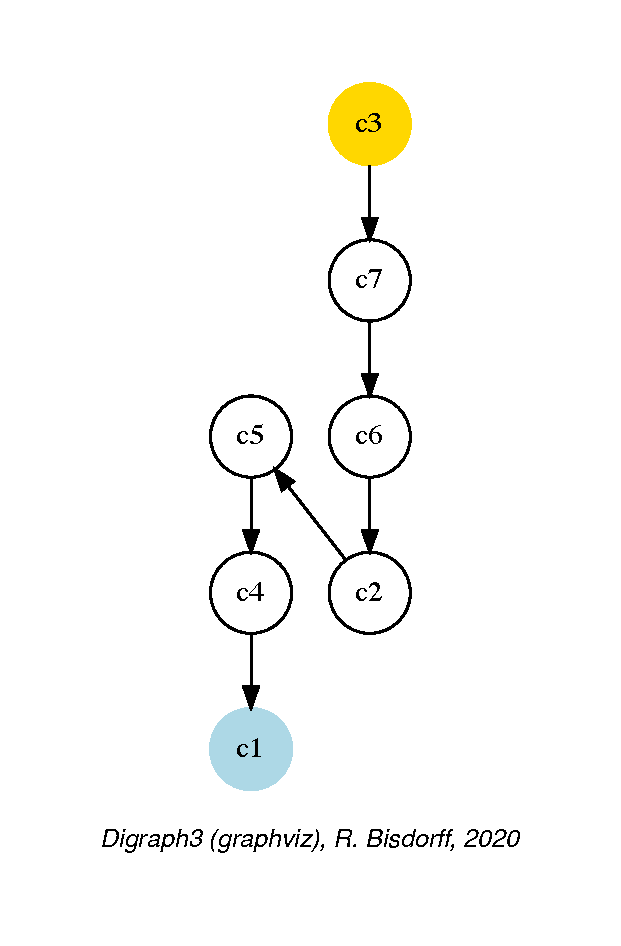
\includegraphics[width=5cm]{Figures/20-2-divGraph.pdf}
\caption{The linear ranking modelled by the majority margins digraph} 
\label{fig:20.2}       % Give a unique label
\end{figure}

\section{Bipolar approval-disapproval voting systems}
\label{sec:20.2}

Traditionally, most of the voting systems in use in the World, do only collect approval votes and abstentions, dismissing potentially strong disapproval opinions, not to be assimilated to voting abstentions. Collecting both explicit approvals ($+1$) and explicit disapprovals ($-1$) essentially enriches the expression of voters' preferences. 

In the \texttt{votingProfiles} module\index{votingProfiles@\texttt{votingProfiles} module} we provide a \texttt{BipolarApprovalVot\-ingProfile} class\index{BipolarApprovalVotingProfile@\texttt{BipolarApprovalVotingProfile} class} for handling voting results where, for each eligible Candidate \texttt{x}, the voters are invited  to \emph{approve} ($+1$), \emph{disapprove} ($-1$), or \emph{ignore} ($0$) the statement that Candidate \texttt{c} should win the election \citep{BAU-2012}.

File \texttt{bpApVotingProfile.py} contains an example of such a approval-disapproval voting profile concerning 100 voters and 15 eligible candidates \footnote{The file \texttt{bpApVotingProfile.py} may be found in the \texttt{examples} directory of the \Digraph resources.}. We can inspect its content with the \texttt{BipolarApprovalVotingProfile} class:\index{BipolarApprovalVotingProfile@\texttt{BipolarApprovalVotingProfile} class}
\begin{lstlisting}[caption={Bipolar approval voting profiles},label=list:20.9]
>>> from votingProfiles import \
...                 BipolarApprovalVotingProfile
>>> bavp = BipolarApprovalVotingProfile('bpApVotingProfile')
>>> bavp
  *------- VotingProfile instance description ------*
    Instance class   : BipolarApprovalVotingProfile
    Instance name    : bpApVotingProfile
    Candidates       : 15
    Voters           : 100
    Attributes       : ['name', 'candidates', 'voters',
                 'approvalBallot', 'netApprovalScores',
                 'ballot']
\end{lstlisting}

Beside the \texttt{candidates} and \texttt{voters} attributes, we discover in Listing~\vref{list:20.10} the \texttt{approvalBallot} attribute which gathers approval-disapproval votes. Its content is the following.
\begin{lstlisting}[caption={Inspecting an approval-disapproval ballot},label=list:20.10]
>>> bavp.approvalBallot
  {'v001':
      {'c01': Decimal('0'),
       ...
       'c04': Decimal('1'), §\label{line:20.10.5}§
       ...
       'c15': Decimal('0')
      },
   'v002':
       {'c01': Decimal('-1'), §\label{line:20.10.10}§
        'c02': Decimal('0'),
        ...
        'c15': Decimal('1')
       },
      ...
   'v100':
     {'c01': Decimal('0'),
      'c02': Decimal('1'),
      ...
      'c15': Decimal('1')
     }
    }
\end{lstlisting}	

Let us denote $A_{\mathtt{v}}$ the set of candidates approved by voter \texttt{v}. In the \texttt{approval\-Ballot} attribute we hence record in fact the bipolar-valued truth characteristic values $r(\mathtt{c} \in A_{\mathtt{v}})$ of the statements that Candidate \texttt{c} \emph{is approved} by voter \texttt{v}. In Listing~\vref{list:20.10} Line~\ref{line:20.10.5}, we observe for instance that voter \texttt{v001} positively approves Candidate \texttt{c04}. And, in Line~\ref{line:20.10.10}, we see that voter \texttt{v002} negatively approves, i.e. positively disapproves Candidate \texttt{c01}.

The \texttt{showApprovalResults()} method\index{showApprovalResults@\texttt{showApprovalResults()}} and the \texttt{showDisapproval\-Re\-sults()} method\index{showDisapprovalResults@\texttt{showDisapprovalResults()}} show how many approvals, respectively disapprovals, each candidate receives.
\begin{lstlisting}
>>> bavp.showApprovalResults()
    Approval results
     Candidate: 'c12' obtains 34 votes §\label{line:avpr.c12}§
     Candidate: 'c05' obtains 30 votes
     Candidate: 'c03' obtains 28 votes
     Candidate: 'c14' obtains 27 votes
     Candidate: 'c11' obtains 27 votes
     Candidate: 'c04' obtains 27 votes
     Candidate: 'c01' obtains 27 votes
     Candidate: 'c13' obtains 24 votes
     Candidate: 'c07' obtains 24 votes
     Candidate: 'c15' obtains 23 votes
     Candidate: 'c02' obtains 23 votes
     Candidate: 'c09' obtains 22 votes
     Candidate: 'c08' obtains 22 votes
     Candidate: 'c10' obtains 21 votes
     Candidate: 'c06' obtains 21 votes
    Total approval votes: 380
    Approval proportion: 380/1500 = 0.25
>>> bavp.showDisapprovalResults()
    Disapproval results
     Candidate: 'c12' obtains 16 votes §\label{line:davpr.c12}§
     Candidate: 'c03' obtains 22 votes
     Candidate: 'c09' obtains 23 votes
     Candidate: 'c04' obtains 24 votes
     Candidate: 'c06' obtains 24 votes
     Candidate: 'c13' obtains 24 votes
     Candidate: 'c11' obtains 25 votes
     Candidate: 'c02' obtains 26 votes
     Candidate: 'c07' obtains 26 votes
     Candidate: 'c08' obtains 26 votes
     Candidate: 'c05' obtains 27 votes
     Candidate: 'c10' obtains 27 votes
     Candidate: 'c14' obtains 27 votes
     Candidate: 'c15' obtains 27 votes
     Candidate: 'c01' obtains 32 votes
    Total disapproval votes: 376
    Disapproval proportion: 376/1500 = 0.25
\end{lstlisting}

In Lines~\ref{line:avpr.c12} and \ref{line:davpr.c12} above, we notice that, of all eligible candidates, it is Candidate \texttt{c12} who receives the highest number of approval votes (34) and the lowest number of disapproval votes (16). Total number of approval, respectively disapproval, votes approaches more or less a proportion of $25\%$ of the $100 \times 15 = 1500$ potential approval votes. About $50\%$ of the latter remain hence ignored. 

When operating now, for each Candidate \texttt{x}, the difference between the number of approval and the number of disapproval votes they receive, we obtain per candidate a corresponding \emph{net approval} score; in fact, the bipolar truth characteristic value of the statement ``\emph{Candidate} \texttt{x} \emph{should win the election}''.
\begin{equation}
r(\text{Candidate x should win the election}) \;=\; \sum_{\mathtt{v}} \big(r(\mathtt{x} \in A_{\mathtt{v}})\big)\;.
\end{equation}

These bipolar characteristic values are stored in the \texttt{netApprovalScores} attribute and may be printed out with the \texttt{showNetApprovalScores()} method\index{showNetApprovalScores@\texttt{showNetApprovalScores()}}:
\begin{lstlisting}
>>> bavp.showNetApprovalScores()
  Net Approval Scores
     Candidate: 'c12' obtains 18 net approvals §\label{line:netapsc:3}§
     Candidate: 'c03' obtains 6 net approvals
     Candidate: 'c05' obtains 3 net approvals
     Candidate: 'c04' obtains 3 net approvals
     Candidate: 'c11' obtains 2 net approvals
     Candidate: 'c14' obtains 0 net approvals
     Candidate: 'c13' obtains 0 net approvals
     Candidate: 'c09' obtains -1 net approvals
     Candidate: 'c07' obtains -2 net approvals
     Candidate: 'c06' obtains -3 net approvals
     Candidate: 'c02' obtains -3 net approvals
     Candidate: 'c15' obtains -4 net approvals
     Candidate: 'c08' obtains -4 net approvals
     Candidate: 'c01' obtains -5 net approvals
     Candidate: 'c10' obtains -6 net approvals
\end{lstlisting}

We observe in Line~\ref{line:netapsc:3} above that Candidate \texttt{c12}, with a net approval score of $34 - 16 = 18$, represents indeed the \emph{best approved} candidate for winning the election. With a net approval score of $28-22 = 6$, Candidate \texttt{c03} appears 2nd-best approved. The net approval scores define hence a potentially weak ranking on the set of eligible election candidates, and the winner(s) of the election is(are) determined by the first-ranked candidate(s).

\section{Pairwise comparison of approval-disapproval votes}
\label{sec:20.3}

The approval votes of each voter define now on the set of eligible candidates three ordered categories: his approved ($+1$), his ignored ($0$) and his disapproved ($-1$) ones. Within each of these three categories we consider the voter's actual preferences as \emph{not communicated}, i.e. as missing data. This gives for each voter a partially determined strict order which we find in the \texttt{ballot} attribute.
\begin{lstlisting}
 >>> bavp.ballot['v001']['c12']
    {'c02': Decimal('1'), 'c11': Decimal('1'),
     'c14': Decimal('1'), 'c04': Decimal('0'),
     'c06': Decimal('1'), 'c05': Decimal('1'),
     'c12': Decimal('0'), 'c13': Decimal('0'),
     'c15': Decimal('1'), 'c01': Decimal('1'),
     'c08': Decimal('1'), 'c07': Decimal('1'),
     'c09': Decimal('0'), 'c03': Decimal('1'),
     'c10': Decimal('0')}
\end{lstlisting}

For voter \texttt{v001}, for instance, the best approved Candidate \texttt{c12} is strictly preferred to Candidates: \texttt{c01}, \texttt{c02}, \texttt{c03}, \texttt{c05}, \texttt{c06}, \texttt{c07}, \texttt{c08}, \texttt{c11}, \texttt{c14} and \texttt{c15}. No candidate is preferred to \texttt{c12} and the comparison with \texttt{c04}, \texttt{c09}, \texttt{c10} and \texttt{c13} is not communicated, hence indeterminate. Mind by the way that the reflexive comparison of \texttt{c12} with itself is, as usual, ignored, i.e. indeterminate. Each voter \texttt{v} defines thus a partially determined transitive strict preference relation denoted $\succ_{\mathtt{v}}$ on the eligible candidates.

For each pair of eligible candidates, we aggregate the previous individual voter's preferences into a truth characteristic of the statement: ``Candidate $x$ is \emph{better approved than} Candidate $y$'', denoted $r(x \succ y)$:
\begin{equation}
  r(x \succ y)\;=\; \sum_{\mathtt{v}} \big(\,r(x \succ_{\mathtt{v}} y)\, \big)\;.
\end{equation}  

We say that Candidate $x$ is \emph{better approved than} Candidate $y$ when $r(x \succ y)\;>\;0$, i.e. there is a majority of voters who approve \emph{more} and disapprove \emph{less} $x$ than $y$. Vice-versa, we say that Candidate $x$ is \emph{not} better approved than Candidate $y$ when $r(x \succ y)\;<\;0$, i.e. there is a majority of voters who disapprove more and approve less $x$ than $y$. This computation is achieved with the \texttt{MajorityMarginsDigraph} constructor.
\begin{lstlisting}
>>> from votingProfiles import MajorityMarginsDigraph
>>> m = MajorityMarginsDigraph(bavp)
>>> m
  *------- Digraph instance description ------*
    Instance class      : MajorityMarginsDigraph
    Instance name       : rel_bpApVotingProfile
    Digraph Order       : 15
    Digraph Size        : 97 §\label{mmdg.8}§
    Valuation domain    : [-100.00;100.00]
    Determinateness (%) : 52.55
    Attributes          : ['name', 'actions',
               'criteria','ballot',
               'valuationdomain', 'relation',
               'order', 'gamma', 'notGamma']
\end{lstlisting}

The resulting digraph \texttt{m} contains 97 positively validated relations (see Line~\ref{mmdg.8} above) and for all pairs $(x,y)$ of eligible candidates, $r(x \succ y)$ takes value in an valuation range from $-100.00$ (unanimously rejected) to $+100.00$ (unanimously approved).

These pairwise $r(x \succ y)$ values can be inspected in a browser view with the \texttt{showHTMLRelationTable()} method: 
\begin{lstlisting}
>>> m.showHTMLRelationTable(relationName='r(x > y)')
\end{lstlisting}
\begin{figure}[ht]
%\sidecaption
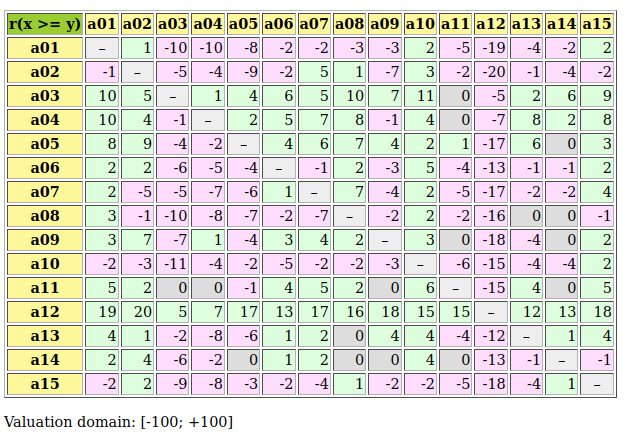
\includegraphics[width=0.8\hsize]{Figures/20-3-majMargAV.png}
\caption{The bipolar-valued pairwise majority margins} 
\label{fig:20.3}       % Give a unique label
\end{figure}

In Fig.~\vref{fig:20.3} it gets apparent that Candidate \texttt{c12} is a \Condorcet winner, i.e. the candidate who beats all the other candidates and, with the given voting profile \texttt{gavp}, should without doubt win the election. This strongly confirms the first-ranked result obtained with the previous net approval scoring. 

Let us eventually compute, with the help of the \NetFlows ranking rule\footnote{See Sect.~\ref{sec:8.3}.}, a linear ranking of the 15 eligible candidates and compare the result with the net approval scores ranking.
\begin{lstlisting}[caption={Comparing the net approval and the \NetFlows rankings},label=list:20.11]
>>> from linearOrders import NetFlowsOrder
>>> nf = NetFlowsOrder(m,Comments=True)
>>> print('NetFlows versus Net Approval Ranking')
>>> print('Candidate\tNetFlows score\tNet Approval score')
>>> for item in nf.netFlows:
...     print( '%9s\t  %+.3f\t %+.1f' %\
...	        (item[1], item[0],\
...              bavp.netApprovalScores[item[1]]) ) 
    NetFlows versus Net Approval Ranking
    Candidate	NetFlows score	Net Approval score
      'c12'	  +410.000	 +18.0
      'c03'	  +142.000	  +6.0
      'c04'	   +98.000	  +3.0
      'c05'	   +54.000	  +3.0
      'c11'	   +34.000	  +2.0
      'c09'	   -16.000	  -1.0 §\label{line:20.11.16}§
      'c14'	   -20.000	  +0.0
      'c13'	   -22.000	  +0.0
      'c06'	   -50.000	  -3.0 §\label{line:20.11.19}§
      'c07'	   -74.000	  -2.0
      'c02'	   -96.000	  -3.0
      'c08'	   -102.000	  -4.0
      'c15'	   -110.000	  -4.0
      'c10'	   -122.000	  -6.0
      'c01'	   -126.000	  -5.0
\end{lstlisting}

In Listing~\vref{list:20.11} we may notice that the \NetFlows rule delivers a ranking that is very similar to the one previously obtained with the corresponding \emph{Net Approval} scores. Only minor inversions do appear, like in the midfield, where Candidate \texttt{c09} advances before Candidates \texttt{c13} and \texttt{c14} (see Line~\ref{line:20.11.16}), and \texttt{c06} and \texttt{c07} swap their positions 9 and 10 (see Line~\ref{line:20.11.19}). The two last-ranked Candidates \texttt{c10} and \texttt{c01} also swap their positions.

This confirms again the pertinence of the net approval scoring approach for finding the winner in an approval-disapproval voting system. Yet, voting by approving ($+1$), disapproving ($-1$) or ignoring ($0$) eligible candidates, may also be seen as a performance evaluation of the eligible candidates on a $\{-1, 0, 1\}$-valued ordinal scale.

\section{Three-valued evaluative voting systems}
\label{sec:20.4}

Following such an epistemic perspective, we may effectively convert the given \texttt{BipolarApprovalVotingProfile} instance into a \texttt{PerformanceTableau} instance, so as to get access to a corresponding outranking decision aiding approach.

Mind that, contrary to the majority margins of the ``\emph{better approved than}'' relation, all voters consider now the approved candidates to be equivalent ($+1$). Same is true for the disapproved ($-1$), respectively the ignored ($0$) candidates. The voter's marginal preferences model this time a complete preorder with three equivalence classes. 

From the saved file \texttt{AVPerfTab.py} (see Line~\ref{line:20.12.1} below), we may construct an outranking relation on the eligible candidates with our standard \texttt{BipolarOutran\-kingDigraph} class constructor. The semantics of this outranking relation are the following:
\begin{itemize}[nosep,leftmargin=0.5cm,rightmargin=0.5cm]
\item We say that Candidate $x$ \emph{outranks} Candidate $y$ when there is a majority of voters who consider $x$ \emph{at least as well evaluated as} $y$;
\item We say that Candidate $x$ is \emph{outranked by} Candidate $y$ when there is a majority of voters who consider $x$ \emph{not at least as well evaluated as} $y$;
\item Otherwise, the outranking situation is indeterminate.
\end{itemize}
\begin{lstlisting}[caption={Computing the outranking digraph},label=list:20.12]
>>> bavp.save2PerfTab(fileName='AVPerfTab',valueDigits=0) §\label{line:20.12.1}§
  *--- Saving as performance tableau in AVPerfTab.py ---*
>>> from outrankingDigraphs import\
...                         BipolarOutrankingDigraph
>>> odg = BipolarOutrankingDigraph('AVPerfTab')
>>> odg
  *------- Object instance description ------*
    Instance class       : BipolarOutrankingDigraph
    Instance name        : rel_AVPerfTab
    Actions              : 15
    Criteria             : 100
    Size                 : 210 §\label{line:20.12.12}§
    Determinateness (%)  : 69.29
    Valuation domain     : [-1.00;1.00]
    Attributes           : ['name', 'actions', 'order,
                       'criteria', 'evaluation', 'NA',
                       'valuationdomain', 'relation',
                       'gamma', 'notGamma', ...]
\end{lstlisting}

The size ($210 = 15 \times 14$) of the resulting outranking digraph \texttt{odg}, shown in Listing~\vref{list:20.12} Line~\ref{line:20.12.12} above, reveals that the corresponding ``\emph{at least as good evaluated as}'' relation models actually a trivial \emph{complete} digraph. All candidates appear to be \emph{equally} at least as well evaluated and the strict ``\emph{better evaluated than}'' (codual) outranking digraph becomes in fact empty. The converted performance tableau does apparently not contain sufficiently discriminatory performance evaluations for supporting any strict preference situations.

Yet, we may nevertheless try to apply again the \NetFlows ranking rule to this complete outranking digraph \texttt{odg} and print side by side the corresponding \NetFlows scores and the previous Net Approval scores. 
\begin{lstlisting}[caption={Comparing the \NetFlows and the Net Approval rankings},label=list:20.13]
>>> from linearOrders import NetFlowsOrder
>>> nf = NetFlowsOrder(odg)
>>> print('NetFlows versus Net Approval Ranking')
>>> print('Candidate\tNetFlows Score\tNet Approval Score')
>>> for item in nf.netFlows:
...     print('%9s\t  %+.3f\t %+.0f' %\
...         (item[1],item[0],\
...          bavp.netApprovalScores[item[1]]) )  
    NetFlows versus Net Approval Ranking
    Candidate    NetFlows score	Net Approval score
      c12	  +4.100	    +18
      c03	  +1.420	     +6
      c04	  +0.980	     +3
      c05	  +0.540             +3
      c11	  +0.340	     +2
      c09	  -0.160	     -1
      c14	  -0.200	      0
      c13	  -0.220	      0
      c06	  -0.500	     -3
      c07	  -0.740	     -2
      c02	  -0.960	     -3
      c08	  -1.020	     -4
      c15	  -1.100	     -4
      c10	  -1.220	     -6
      c01	  -1.260	     -5
\end{lstlisting}

Despite its apparent poor strict preference discriminating power, we obtain in Listing~\vref{list:20.13} here \NetFlows scores that are directly proportional (divided by $100$) to the scores obtained with the \emph{better approved than} majority margins digraph \texttt{m} (see List.~\vref{list:20.11}).

Encouraged by this positive result, we may furthermore compute a \Rubis best choice recommendation (see Chap.~\ref{sec:4}).
\begin{lstlisting}[caption={Computing a best social choice recommendation},label=list:20.14]
>>> odg.showBestChoiceRecommendation()
  Rubis best choice recommendation(s) (BCR)
   (in decreasing order of determinateness)   
   Credibility domain: [-1.00,1.00]
  === >> ambiguous first choice(s) 
   * choice        : ['c01','c02','c03','c04','c05', §\label{line:20.14.6}§
                      'c06','c07','c08','c09','c10',
                      'c11','c12','c13','c14','c15'] §\label{line:20.14.8}§
    independence   : 0.06
    dominance      : 1.00
    absorbency     : 1.00
    covering (%)   : 100.00
    determinateness (%) : 61.13
    - most credible action(s) = {
        'c12': 0.44, 'c03': 0.34, 'c04': 0.30, §\label{line:20.14.15}§
        'c14': 0.28, 'c13': 0.24, 'c06': 0.24,
        'c11': 0.20, 'c10': 0.20, 'c07': 0.20,
        'c01': 0.20, 'c08': 0.18, 'c05': 0.18,
        'c15': 0.14, 'c09': 0.14, 'c02': 0.06, }
   === >> ambiguous last choice(s)
    * choice        : ['c01','c02','c03','c04','c05',
                      'c06','c07','c08','c09','c10',
                      'c11','c12','c13','c14','c15']
     independence   : 0.06
     dominance      : 1.00
     absorbency     : 1.00
     covered (%)    : 100.00
     determinateness (%) : 63.73
     - most credible action(s) = {
         'c13': 0.36, 'c06': 0.36, 'c15': 0.34, §\label{line:20.14.30}§
         'c01': 0.34, 'c08': 0.32, 'c07': 0.30,
         'c02': 0.30, 'c14': 0.28, 'c11': 0.28,
         'c09': 0.28, 'c04': 0.26, 'c10': 0.24,
         'c05': 0.20, 'c03': 0.20, 'c12': 0.06, }
\end{lstlisting}

The strict outranking digraph $(\sim (-odg))$ being actually $empty$, we obtain a unique \emph{ambiguous} --first as well as last-- choice recommendation which trivially retains all fifteen candidates (see List.~\vref{list:20.14} Lines~\ref{line:20.14.6}-\ref{line:20.14.8} above). Yet, the bipolar-valued best choice membership characteristic vector reveals that, among all the fifteen potential winners, it is indeed Candidate \texttt{c12} the most credible one with a $72\%$ majority of voters' support (see Line~\ref{line:20.14.15}, $(0.44 + 1.0)/2\;=\; 0.72$); followed by Candidate \texttt{c03} ($67\%$) and Candidate \texttt{c04} ($65\%$). Similarly, Candidates \texttt{c13} and \texttt{c06} represent the most credible losers with a $68\%$ majority voters' support (Line~\ref{line:20.14.30}).

We observe here empirically that \emph{evaluative} voting systems, using three-valued ordinal performance scales, match closely corresponding approval-disapproval voting systems. The latter systems model, however, more faithfully the very preferential information that is expressed with \emph{approved}, \emph{disapproved} and \emph{ignored} statements. The corresponding evaluation on a three-level scale, being value (numbers) based, cannot express the fact that in approval-disapproval voting system there is no preferential information given concerning the pairwise comparison of all approved, respectively disapproved or ignored candidates.

Let us finally illustrate how approval-disapproval voting systems may favour multipartisan supported candidates. We shall therefore compare \emph{approval-disapproval} versus \emph{uninominal plurality} election results when considering a highly divisive and partisan political context.
 
\section{Favouring multipartisan candidates}
\label{sec:20.5}

In modern democracy, politics  are largely structured by political parties and activists. Let us so consider an approval-disapproval voting profile \texttt{dvp} where the random voter behaviour is simulated from two pre-electoral polls concerning a political scene with essentially two major highly competing parties, like the one existing in the US.
\begin{lstlisting}[caption={A random approval-disapproval voting profile in a divisive political context},label=list:20.15]
>>> dvp = RandomBipolarApprovalVotingProfile(\
...                numberOfCandidates=15,\
...                numberOfVoters=100,
...                approvalProbability=0.25,
...                disapprovalProbability=0.25,
...                WithPolls=True,
...                partyRepartition=0.5,
...                other=0.05,
...                DivisivePolitics=True,
...                seed=200)
>>> dvp.showRandomPolls()
  Random repartition of voters
  Party-1 supporters : 45 (45.00%)
  Party-2 supporters : 49 (49.00%)
  Other voters       : 6 (06.00%)
  *---------------- random polls -----------------
  Party-1(45.0%) | Party-2(49.0%) |   expected  
  ------------------------------------------------
  'c05' : 24.10% | 'c07' : 24.10% | 'c07' : 11.87%
  'c14' : 23.48% | 'c10' : 23.48% | 'c10' : 11.60%
  'c03' : 15.13% | 'c01' : 15.13% | 'c05' : 10.91%
  'c12' : 07.55% | 'c04' : 07.55% | 'c14' : 10.67%
  'c08' : 07.11% | 'c09' : 07.11% | 'c01' : 07.67%
  'c15' : 04.37% | 'c13' : 04.37% | 'c03' : 07.09%
  'c11' : 03.99% | 'c02' : 03.99% | 'c04' : 04.55%
  'c06' : 03.80% | 'c06' : 03.80% | 'c09' : 04.49%
  'c02' : 02.79% | 'c11' : 02.79% | 'c12' : 04.32%
  'c13' : 02.63% | 'c15' : 02.63% | 'c08' : 04.30%
  'c09' : 02.24% | 'c08' : 02.24% | 'c06' : 03.57%
  'c04' : 01.89% | 'c12' : 01.89% | 'c13' : 03.32%
  'c01' : 00.57% | 'c03' : 00.57% | 'c15' : 03.25%
  'c10' : 00.20% | 'c14' : 00.20% | 'c02' : 03.21%
  'c07' : 00.14% | 'c05' : 00.14% | 'c11' : 03.16%
\end{lstlisting}   

In Listing~\vref{list:20.15}, the divisive political situation is reflected by the fact that Party-1 and Party-2 supporters show strict opposite preferences. The leading candidates of Party-1 (\texttt{c05} and \texttt{c14}) are last choices for Party-2 supporters and, Candidates \texttt{c07} and \texttt{c10}, leading candidates for Party-2 supporters, are similarly the least choices for Party-1 supporters.

No clear winner may be guessed from these pre-election polls. As Party-2 shows however slightly more supporters than Party-1, the expected winner in an uninominal plurality or instant-run-off voting system will be Candidate \texttt{c07}, i,e, the leading candidate of majority Party-2 (see below).
\begin{lstlisting}
>>> dvp.computeSimpleMajorityWinner()
  ['c07']
>>> dvp.computeInstantRunoffWinner()
  ['c07']
\end{lstlisting}

Now, in a corresponding approval-disapproval voting system, Party-1 supporters will usually approve their leading candidates and disapprove the leading candidates of Party-2. Vice versa, Party-2 supporters will usually approve their leading candidates and disapprove the leading candidates of Party-1. Let us consult the resulting approval votes per candidate.
\begin{lstlisting}
>>> dvp.showApprovalResults()
     Candidate: 'c07' obtains 30 votes
     Candidate: 'c10' obtains 28 votes
     Candidate: 'c05' obtains 28 votes
     Candidate: 'c01' obtains 28 votes
     Candidate: 'c03' obtains 26 votes
     Candidate: 'c02' obtains 26 votes
     Candidate: 'c12' obtains 25 votes
     Candidate: 'c14' obtains 24 votes
     Candidate: 'c13' obtains 24 votes
     Candidate: 'c09' obtains 21 votes
     Candidate: 'c04' obtains 21 votes
     Candidate: 'c08' obtains 19 votes
     Candidate: 'c06' obtains 17 votes
     Candidate: 'c15' obtains 15 votes
     Candidate: 'c11' obtains 12 votes
    Total approval votes: 344
    Approval proportion: 344/1500 = 0.23
\end{lstlisting}

When considering only the approval votes, we find confirmed above that the leading candidate of Party-2 obtains in this simulation a plurality of approval votes. In uninominal plurality or instant-runoff voting systems, this candidate wins hence the election, quite to the despair of Party-1 supporters. As a foreseeable consequence, this election result will be more or less aggressively contested which leads to a loss of popular trust in democratic elections and institutions.

If we look however on the corresponding disapprovals, we discover that, not surprisingly, the leading candidates of both parties collect by far the highest number of disapproval votes. 
\begin{lstlisting}
>>> dvp.showDisapprovalResults()
     Candidate: 'c02' obtains 14 votes
     Candidate: 'c04' obtains 14 votes
     Candidate: 'c13' obtains 14 votes
     Candidate: 'c06' obtains 15 votes
     Candidate: 'c09' obtains 15 votes
     Candidate: 'c08' obtains 16 votes
     Candidate: 'c11' obtains 16 votes
     Candidate: 'c15' obtains 18 votes
     Candidate: 'c12' obtains 20 votes
     Candidate: 'c01' obtains 29 votes
     Candidate: 'c03' obtains 30 votes
     Candidate: 'c10' obtains 37 votes
     Candidate: 'c07' obtains 44 votes
     Candidate: 'c14' obtains 45 votes
     Candidate: 'c05' obtains 49 votes
    Total disapproval votes: 376
    Disapproval proportion: 376/1500 = 0.25
\end{lstlisting}

Balancing now approval against disapproval votes will favour the moderate, bipartisan supported, candidates.
\begin{lstlisting}
>>> dvp.showNetApprovalScores()
    Net Approval Scores
     Candidate: 'c02' obtains 12 net approvals
     Candidate: 'c13' obtains 10 net approvals
     Candidate: 'c04' obtains 7 net approvals
     Candidate: 'c09' obtains 6 net approvals
     Candidate: 'c12' obtains 5 net approvals
     Candidate: 'c08' obtains 3 net approvals
     Candidate: 'c06' obtains 2 net approvals
     Candidate: 'c01' obtains -1 net approvals
     Candidate: 'c15' obtains -3 net approvals
     Candidate: 'c11' obtains -4 net approvals
     Candidate: 'c03' obtains -4 net approvals
     Candidate: 'c10' obtains -9 net approvals
     Candidate: 'c07' obtains -14 net approvals
     Candidate: 'c14' obtains -21 net approvals
     Candidate: 'c05' obtains -21 net approvals
\end{lstlisting}

Candidate \texttt{c02}, appearing in the pre-electoral polls in the midfield (in position 7 for Party-2 and in position 9 for Party-1 supporters, see List.\vref{list:20.15}), shows indeed the highest net approval score. Second highest net approval score obtains Candidate \texttt{c13}, in  position 6 for Party-2 and in position 10 for Party-1 supporters.

Figure~\vref{fig:20.4}, showing the \NetFlows ranked relation table of the ``\emph{better approved than}'' majority margins digraph, confirms below this net approval scoring result.
\begin{lstlisting}
>>> m = MajorityMarginsDigraph(dvp)
>>> m.showHTMLRelationTable(\
...      actionsList=m.computeNetFlowsRanking(),
...      relationName='r(x > y)')
\end{lstlisting}	   
\begin{figure}[ht]
%\sidecaption
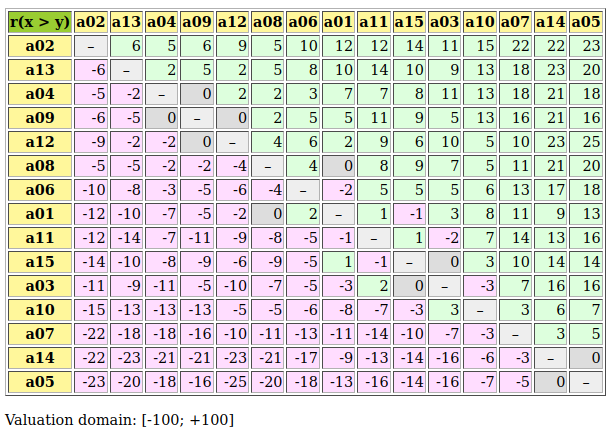
\includegraphics[width=0.8\hsize]{Figures/20-4-majMargDAV.png}
\caption{The pairwise \emph{better approved than} majority margins} 
\label{fig:20.4}       % Give a unique label
\end{figure}

Candidate \texttt{c02} appears indeed \emph{better approved than} any other candidate (\Condorcet winner); and, the leading Candidates of Party-1, \texttt{c05} and \texttt{c14}, are \emph{less approved than} any other candidates (weak \Condorcet losers).
\begin{lstlisting}
>>> m.computeCondorcetWinners()
  ['c02']
>>> m.computeWeakCondorcetLosers()
  ['c05','c14']
\end{lstlisting}

We see this result furthermore confirmed when computing the corresponding first, respectively last choice recommendation.    
\begin{lstlisting}
>>> m.showBestChoiceRecommendation()
  Rubis best choice recommendation(s) (BCR)
   (in decreasing order of determinateness)   
   Credibility domain: [-100.00,100.00]
   === >> potential first choice(s)
    * choice              : ['c02']
      independence        : 100.00
      dominance           : 5.00
      absorbency          : -23.00
      covering (%)        : 100.00
      determinateness (%) : 52.50
      - most credible action(s) = { 'c02': 5.00, }
   === >> potential last choice(s) 
    * choice              : ['c05', 'c14']
      independence        : 0.00
      dominance           : -23.00
      absorbency          : 5.00
      covered (%)         : 100.00
      determinateness (%) : 50.00
      - most credible action(s) = { }
\end{lstlisting}

Candidate \texttt{c02}, being actually a \Condorcet winner, gives an initial prekernel of digraph \texttt{m}, whereas Party-1 leading Candidates \texttt{c05} and \texttt{c14}, both being weak \Condorcet losers, give together a terminal prekernel. They hence represent our \emph{first choice}, respectively, \emph{last choice} recommendations for winning this simulated election.

It is worthwhile noticing again the essential structural and computational role, the ignored value is playing in approval-disapproval voting systems. This epistemic and logical \emph{neutral} term is needed indeed for handling in a consistent and efficient manner \emph{not communicated votes} and/or \emph{indeterminate} preferential statements.

Let us conclude by predicting that, for leading political candidates in an aggressively divisive political context, the perspective to easily fail election withan approval-disapproval voting system, might or will induce a change in the usual way of running electoral campaigns. Political parties and politicians, who avoid aggressive competitive propaganda and instead propose multipartisan collaborative social choices, will be rewarded with better election results than any kind of extremism. It could mean the end of sterile political obstructions and war like electoral battles. \emph{Let's do it !}.

\vspace{\baselineskip}
The last Part V of this monograph illustrates in three chapters computational resources for working with simple undirected graphs.

%%%%%%% The chapter bibliography
%\normallatexbib
%\clearpage
%\phantomsection
%\addcontentsline{toc}{section}{Chapter Bibliography}
\chapter{Tempering plurality tyranny effects in social choice}
\label{sec:20}


\abstract*{ In a \emph{social choice} context, where decision objectives would match different political parties, Pareto efficient choice recommendations represent in fact \emph{multipartisan} social choices that may judiciously deliver the primary selection in a two stage election system. Our bipolar-valued outranking model is based on approvals-disapprovals of ``\emph{at least as well evaluated as}'' statements. A similar approach is put into practice with approval-disapproval voting systems. When converting such approval-disapproval voting ballots into corresponding performance records, we obtain a $(-1,0,1)$-valued evaluative voting system. We eventually show that in such a approval-disapproval voting system, the winner tends to be among the more or less multipartisan candidates.}

\begin{quotation}\emph{The choice of a voting procedure shapes the democracy in which we live}.\\
    -- \citet*{BAU-2012}.
\end{quotation}
\vspace{1cm}

\abstract{ In a \emph{social choice} context, where decision objectives would match different political parties, Pareto efficient choice recommendations represent in fact \emph{multipartisan} social choices that may judiciously deliver the primary selection in a two stage election system. Our bipolar-valued outranking model is based on approvals-disapprovals of ``\emph{at least as well evaluated as}'' statements. A similar approach is put into practice with approval-disapproval voting systems. When converting such approval-disapproval voting ballots into corresponding performance records, we obtain a $(-1,0,1)$-valued evaluative voting system. We eventually show that in such a approval-disapproval voting system, the winner tends to be among the more or less multipartisan candidates.}

\paragraph{\textbf{Introduction}}

From the seminal work by \emph{Bernard Roy}\index{Roy@\textsl{B. Roy}} on, tempering plurality tyranny effects is achieved in the outranking approach by taking into account considerable negative performance differences that render doubtful otherwise positive ``\emph{at least as well evaluated as}'' situations \citep*{ROY-1966}. In the social choice context of general elections, such a polarisation is not feasible as the genuine uninominal voting ballots do not contain a rich enough preferential information. Yet, when matching decision objectives with political parties, the Pareto efficient outranking situations seen in Sect.~\ref{sec:19.6}, correspond to multipartisan ``\emph{at least as well approved as}'' situations when pairwisely comparing the eligible candidates. A best choice recommendation based of the corresponding multipartisan strict ``\emph{better approved as}'' situations may, the case given, deliver a convincing primary selection in a two-stage election. 

\section{Two-stage elections with multipartisan primary selection}
\label{sec:20.1}

To compute multipartisan social choices we need to, first, convert a given linear voting profile with pre-election polls into a corresponding performance tableau. We shall illustrate this point with a voting profile we discussed already in Chap.~\ref{sec:7}.
\begin{lstlisting}[caption={Example of a 3 parties voting profile},label=list:20.1]
>>> from votingProfiles import RandomLinearVotingProfile
>>> lvp = RandomLinearVotingProfile(numberOfCandidates=15,
...                         numberOfVoters=1000,
...                         WithPolls=True,
...                         partyRepartition=0.5,
...                         other=0.1,
...                         seed=0.9189670954954139)
>>> lvp
  *------- VotingProfile instance description ------*
   Instance class   : RandomLinearVotingProfile
   Instance name    : randLinearProfile
   Candidates       : 15
   Voters           : 1000
   Attributes       : ['name', 'seed', 'candidates',
             'voters', 'WithPolls', 'RandomWeights',
             'sumWeights', 'poll1', 'poll2',
             'other', partyRepartition,
             'linearBallot', 'ballot']
>>> lvp.showRandomPolls() §\label{line:20.1.20}§
  Random repartition of voters
   Party_1 supporters : 460 (46.0%)
   Party_2 supporters : 436 (43.6%)
   Other voters       : 104 (10.4%)
  *---------------- random polls ----------------
   Party-1(46.0%) | Party-(43.6%)|  expected  
   ----------------------------------------------
    c06 : 19.91%  | c11 : 22.94%  | c06 : 15.00%
    c07 : 14.27%  | c08 : 15.65%  | c11 : 13.08%
    c03 : 10.02%  | c04 : 15.07%  | c08 : 09.01%
    c13 : 08.39%  | c06 : 13.40%  | c07 : 08.79%
    c15 : 08.39%  | c03 : 06.49%  | c03 : 07.44%
    c11 : 06.70%  | c09 : 05.63%  | c04 : 07.11%
    c01 : 06.17%  | c07 : 05.10%  | c01 : 05.06%
    c12 : 04.81%  | c01 : 05.09%  | c13 : 05.04%
    c08 : 04.75%  | c12 : 03.43%  | c15 : 04.23%
    c10 : 04.66%  | c13 : 02.71%  | c12 : 03.71%
    c14 : 04.42%  | c14 : 02.70%  | c14 : 03.21%
    c05 : 04.01%  | c15 : 00.86%  | c09 : 03.10%
    c09 : 01.40%  | c10 : 00.44%  | c10 : 02.34%
    c04 : 01.18%  | c05 : 00.29%  | c05 : 01.97%
    c02 : 00.90%  | c02 : 00.21%  | c02 : 00.51% §\label{line:20.1.end}§
\end{lstlisting}

In this example (see List.~\vref{list:20.1} Lines~\ref{line:20.1.20}-\ref{line:20.1.end}), we observe 460 Party-1 supporters ($46\%$), 436 Party-2 supporters ($43.6\%$) and 104 other voters ($10.4\%$). Favorite candidates of Party-1 supporters, with more than $10\%$, are \texttt{c06} ($19.91\%$), \texttt{c07} ($14.27\%$) and \texttt{c03} ($10.02\%$). Whereas for Party-2 supporters, favorite candidates are \texttt{c11} ($22.94\%$), followed by \texttt{c08} ($15.65\%$), \texttt{c04} ($15.07\%$) and \texttt{c06} ($13.4\%$).

We can convert this linear voting profile into a \texttt{PerformanceTableau} object where each political party matches a decision objective.
\begin{lstlisting}[caption={Converting a voting profile into a performance tableau},label=list:20.2]
>>> lvp.save2PerfTab('votingPerfTab')§\label{line:20.2.1}§
>>> from perfTabs import PerformanceTableau
>>> vpt = PerformanceTableau('votingPerfTab')§\label{line:20.2.3}§
>>> vpt
  *------- PerformanceTableau instance description ---*
    Instance class   : PerformanceTableau
    Instance name    : votingPerfTab
    Actions          : 15
    Objectives       : 3
    Criteria         : 1000
    Attributes       : ['name', 'actions', 'objectives',
              'criteria', 'weightPreorder', 'evaluation']
>>> vpt.objectives
  OrderedDict([
    ('party0', {'name': 'other', 'weight': Decimal('104'),
     'criteria': ['v0003', 'v0008', 'v0011', ... ']}),
    ('party1', {'name': 'party 1', 'weight': Decimal('460'),
     'criteria': ['v0002', 'v0006', 'v0007', ...]}),
    ('party2', {'name': 'party 2', 'weight': Decimal('436'),
      'criteria': ['v0001', 'v0004', 'v0005', ... ]})
    ])
\end{lstlisting}

In Listing~\vref{list:20.2} the linear voting profile lvp is first stored in \texttt{Performance\-Tableau} format (see Line~\ref{line:20.2.1}). In Line~\ref{line:20.2.3}, the PerformanceTableau class reloads this stored performance tableau data. The three parties of the linear voting profile represent three decision objectives and the 1000 voters are distributed as 1000 performance criteria according to the party they support.

In order to operate now a \emph{primary multipartisan selection} of potential election winners, we compute the corresponding unopposed multiobjective outranking digraph (see Sect.~\ref{sec:19.5}).
\begin{lstlisting}[caption={Computing unopposed multiobjective outranking situations},label=list:20.3]
>>> from outrankingDigraphs import \
...       UnOpposedBipolarOutrankingDigraph
>>> uog = UnOpposedBipolarOutrankingDigraph(vpt)
>>> uog
  *------- Object instance description ------*
    Instance class      : UnOpposedBipolarOutrankingDigraph
    Instance name       : unopposed_outrankings
    Actions             : 15
    Criteria            : 1000
    Size                : 34
    Oppositeness (%)    : 67.31 §\label{line:20.3.opp}§
    Determinateness (%) : 57.61
    Valuation domain    : [-1.00;1.00]
    Attributes          : ['name', 'actions', 'valuationdomain',
                           'objectives', 'criteria', 'methodData',
                           'evaluation', 'order', 'runTimes',
                           'relation', 'marginalRelationsRelations',
                           'gamma', 'notGamma']
\end{lstlisting}

From the potential 105 pairwise outranking situations, we keep 34 positively validated outranking situations, leading to a degree of \emph{oppositeness} between political parties of $67.31\%$ (see List.~\ref{list:20.3} Line~\ref{line:20.3.opp}).

The corresponding bipolar-valued relation table can be shown by orienting the list of candidates with the help of the initial and terminal prekernels.\index{showPreKernels@\texttt{showPreKernels()}}
\begin{lstlisting}[caption={Computing unopposed multiobjective outranking situations},label=list:20.4]
>>> uog.showPreKernels()
  *--- Computing preKernels ---*
   Dominant preKernels :
    ['c11', 'c06', 'c13', 'c15']
       independence :  0.0
       dominance    :  0.18
       absorbency   :  -0.66
       covering     :  0.43
   Absorbent preKernels :
    ['c02', 'c04', 'c14', 'c03']
       independence :  0.0
       dominance    :  0.0
       absorbency   :  0.37
       covered      :  0.46
>>> orientedCandidatesList = ['c06','c11','c13','c15',\
...         'c01','c05','c07','c08','c09','c10','c12',\
...         'c02','c03','c04','c14']
>>> uog.showHTMLRelationTable(\
...    actionsList=orientedCandidatesList,\
...    tableTitle='Unopposed three-partisan outrankings')
\end{lstlisting}

\begin{figure}[ht]
%\sidecaption
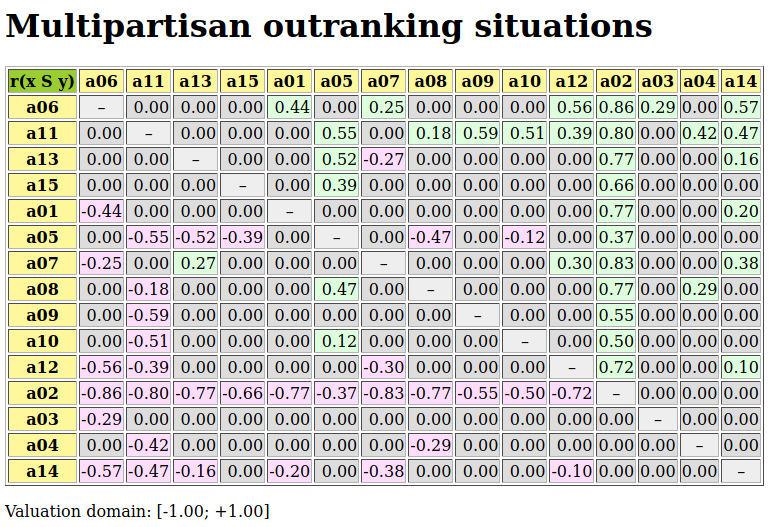
\includegraphics[width=0.9\hsize]{Figures/20-1-unOpposedOutrankings.png}
\caption{Relation table of multipartisan outranking digraph} 
\label{fig:20.1}       % Give a unique label
\end{figure}

In Fig.~\vref{fig:20.1}, we may notice that the dominating outranking prekernel \{\texttt{c06}, \texttt{c11}, \texttt{c13}, \texttt{c15}\} gathers in fact a multipartisan selection of potential election winners. It is worthwhile noticing that the majority margins obtained from a linear voting profile do verify the zero-sum rule: $\big(\,r(x \succsim y) \,+\, r(y \succsim x) \;=\; 0.0\,\big)$. To each positive outranking situation corresponds an equivalent negative converse situation and the resulting outranking and strict outranking digraphs are the same.

When restricting now, in a secondary election stage, the set of eligible candidates to this dominating prekernel, we may compute the actual best social choice.
\begin{lstlisting}[caption={Recommending the secondary election winner},label=list:20.5]
>>> from outrankingDigraphs import BipolarOutrankingDigraph
>>> g2 = BipolarOutrankingDigraph(vpt,\
..          actionsSubset=['c06','c11','c13','c15'])
>>> g2.showRelationTable(ReflexiveTerms=False)
  * ---- Relation Table -----
     r    | 'c06'  'c11'  'c13'  'c15'   
    ------|----------------------------
    'c06' |   -    +0.10  +0.48  +0.52  §\label{line:20.5.8}§
    'c11' | -0.10    -    +0.27  +0.29  
    'c13' | -0.48  -0.27    -    +0.19  
    'c15' | -0.52  -0.29  -0.19    -    §\label{line:20.5.11}§
    Valuation domain: [-1.0; 1.0]
>>> g2.computeCondorcetWinners()
  ['c06']
>>> g2.computeCopelandRanking()
  ['c06', 'c11', 'c13', 'c15']
\end{lstlisting}

Candidate \texttt{c06} appears clearly to be the winner of this election. Notice by the way that the restricted pairwise outranking relation, shown in Listing~\ref{list:20.5} Lines~\ref{line:20.5.8}-\ref{line:20.5.11}, models a linear ordering of the preselected candidates.

We can eventually check the quality of this best choice by noticing that Candidate \texttt{c06} represents indeed the \emph{simple majority}, the \emph{instant runoff}, the \Borda, as well as the \Condorcet winner of the initially given linear voting profile \texttt{lvp}.
\begin{lstlisting}
>>> lvp.computeSimpleMajorityWinner()
  ['c06']
>>> lvp.computeInstantRunoffWinner()
  ['c06']
>>> lvp.computeBordaWinners()
  ['c06']
>>> from votingProfiles import MajorityMarginsDigraph
>>> cd = MajorityMarginsDigraph(lvp)
>>> cd.computeCondorcetWinners()
  ['c06']
\end{lstlisting}

In our example voting profile here, the multipartisan primary selection stage appears quite effective in reducing the number of eligible candidates to four out of a set of 15 candidates without by the way rejecting the actual winning candidate.

However, in a very \emph{divisive} two major parties system, like in the US, where preferences of the supporters of one major party are opposite to the preferences of the supporters of the other major party, the multipartisan outranking digraph will become nearly indeterminate.

In Listing~\vref{list:20.6} below we generate such a divisive kind of linear voting profile with the help of the \texttt{DivisivePolitics} flag (see Lines~\ref{line:20.6.4} and \ref{line:20.6.14}-\ref{line:20.6.20}). When now converting the voting profile into a performance tableau (Lines 20-21), we can compute the corresponding unopposed outranking digraph.
\begin{lstlisting}[caption={A divisive two-party example of a random linear voting profile},label=list:20.6]
>>> from votingProfiles import RandomLinearVotingProfile		     
>>> lvp = RandomLinearVotingProfile(\
...      numberOfCandidates=7,numberOfVoters=500,\
...      WithPolls=True, partyRepartition=0.4,other=0.2,\ §\label{line:20.6.4}§
...      DivisivePolitics=True, seed=1)
>>> lvp.showRandomPolls()
  Random repartition of voters
   Party-1 supporters : 240 (48.00%)
   Party-2 supporters : 160 (32.00%)
   Other voters       : 100 (20.00%)
  *---------------- random polls -------------
   Party_1(48.0%) | Party_2(32.0%) | expected  
   -------------------------------------------
   c2 : 30.84%    |  c1 : 30.84%   | c2 : 15.56% §\label{line:20.6.14}§
   c3 : 23.67%    |  c4 : 23.67%   | c3 : 12.91%
   c7 : 17.29%    |  c6 : 17.29%   | c7 : 11.43%
   c5 : 11.22%    |  c5 : 11.22%   | c1 : 11.00%
   c6 : 09.79%    |  c7 : 09.79%   | c6 : 10.23%
   c4 : 04.83%    |  c3 : 04.83%   | c4 : 09.89%
   c1 : 02.37%    |  c2 : 02.37%   | c5 : 08.98% §\label{line:20.6.20}§
>>> lvp.save2PerfTab('divisiveExample')
>>> dvp = PerformanceTableau('divisiveExample')
>>> from outrankingDigraphs import \
...        UnOpposedBipolarOutrankingDigraph
>>> uodg = UnOpposedBipolarOutrankingDigraph(dvp)
>>> uodg
  *------- Object instance description ------*
   Instance class : UnOpposedBipolarOutrankingDigraph
   Instance name  : divisiveExample
   Actions        : 7
   Criteria       : 500
   Size           : 0 §\label{line:20.6.32}§
   Oppositeness (%)    : 100.00 §\label{line:20.6.33}§
   Determinateness (%) : 50.00
   Valuation domain    : [-1.00;1.00]
\end{lstlisting}

With an oppositeness degree of $100.0\%$ (see List.~\vref{list:20.6} Lines~\ref{line:20.6.32}-\ref{line:20.6.33}), the preferential disagreement between the political parties is complete, and the unopposed outranking digraph \texttt{uodg} becomes completely indeterminate as shown in the relation table below.
\begin{lstlisting}
>>> uodg.showRelationTable(ReflexiveTerms=False)
  * ---- Relation Table -----
   r   | 'c1'   'c2'  'c3'  'c4'  'c5'  'c6'  'c7'   
  -----|------------------------------------------
  'c1' |   -   +0.00 +0.00 +0.00 +0.00 +0.00 +0.00  
  'c2' | +0.00   -   +0.00 +0.00 +0.00 +0.00 +0.00  
  'c3' | +0.00 +0.00   -   +0.00 +0.00 +0.00 +0.00  
  'c4' | +0.00 +0.00 +0.00   -   +0.00 +0.00 +0.00  
  'c5' | +0.00 +0.00 +0.00 +0.00   -   +0.00 +0.00  
  'c6' | +0.00 +0.00 +0.00 +0.00 +0.00   -   +0.00  
  'c7' | +0.00 +0.00 +0.00 +0.00 +0.00 +0.00   -   
  Valuation domain: [-1.0; 1.0]
\end{lstlisting}      

As a consequence, a multipartisan primary selection, computed with a \texttt{show\-Best\-ChoiceRecommendation()} method,  will keep the complete initial set of eligible candidates and, hence, become \emph{ineffective} (see List.~\vref{list:20.7} Line~\ref{line:20.7.6}).
\begin{lstlisting}[caption={Example of ineffective primary multipartisan selection},label=list:20.7]
>>> uodg.showBestChoiceRecommendation()
  Rubis best choice recommendation(s) (BCR)
   (in decreasing order of determinateness)   
   Credibility domain: [-1.00,1.00]
   === >> ambiguous choice(s)
    choice              : ['c1','c2','c3','c4','c5','c6','c7'] §\label{line:20.7.6}§
    independence        : 0.00
    dominance           : 1.00
    absorbency          : 1.00
    covered (%)         : 100.00
    determinateness (%) : 50.00
     - most credible action(s) = { }
\end{lstlisting}

With such kind of divisive voting profile, there may indeed not always exist an obvious winner. In Listing~\vref{list:20.8}, we see, for instance, that the simple majority winner is \texttt{c2} (Line~\ref{line:20.8.2}), whereas the instant-run-off winner is \texttt{c6} (Line~\ref{line:20.8.4}).
\begin{lstlisting}[caption={Example of non obvious secondary selection},label=list:20.8]
>>> lvp.computeSimpleMajorityWinner()
  ['c2'] §\label{line:20.8.2}§
>>> lvp.computeInstantRunoffWinner()
  ['c6'] §\label{line:20.8.4}§
>>> from votingProfiles import MajorityMarginsDigraph
>>> cg = MajorityMarginsDigraph(lvp) §\label{line:20.8.6}§
>>> cg.showRelationTable(ReflexiveTerms=False)
  * ---- Relation Table -----
    r()  |  'c1' 'c2' 'c3' 'c4' 'c5' 'c6' 'c7'	  
   ------|------------------------------------
    'c1' |   -   -68  -90  -46  -68  -88  -84	 
    'c2' |  +68   -   -32  +80  +46   -6  -24	 
    'c3' |  +90  +32   -   +58  +46   +4   +8 §\label{line:20.8.13}§	 
    'c4' |   +4  -80  -58   -   -16  -68  -72	 
    'c5' |  +68  -46  -46  +16	 -   -26  -64	 
    'c6' |  +88   +6   -4  +68	+26   -    -2	 
    'c7' |  +84  +24   -8  +72	+64   +2   - 	 
Valuation domain: [-500;+500]
>>> cg.computeCondorcetWinners()
  ['c3'] §\label{line:20.8.20}§
>>> lvp.computeBordaWinners()
  ['c3','c7'] §\label{line:20.8.22}§
>>> cg.computeCopelandRanking()
  ['c3', 'c7', 'c6', 'c2', 'c5', 'c4', 'c1'] §\label{line:20.8.24}§
\end{lstlisting}

But in our example here, we are lucky. When constructing with the pairwise majority margins digraph (Line~\ref{line:20.8.6}), a \Condorcet winner, namely \texttt{a3}, becomes apparent (Lines~\ref{line:20.8.13} and \ref{line:20.8.20}), which is also one of the two \Borda winners (Line~\ref{line:20.8.22}). More interesting even is to notice that the apparent majority margins digraph models in fact a linear ranking [\texttt{a3}, \texttt{a7}, \texttt{a6}, \texttt{a2}, \texttt{a5}, \texttt{a4}, \texttt{a1}] of all the eligible candidates, as shown with a \Copeland ranking rule (Line~\ref{line:20.8.24}).

In Fig.~\vref{fig:20.2}, this linear ranking is shown with a graphviz drawing where all transitive arcs are dropped and the drawing is oriented with the \Condorcet winner \texttt{a3} and loser \texttt{a1} (Line~\ref{line:fl.3} below).
\begin{lstlisting}
>>> cg.closeTransitive(Reverse=True)
>>> cg.exportGraphViz('divGraph',\
...            firstChoice=['c3'],lastChoice=['c1']) §\label{line:fl.3}§
  *---- exporting a dot file for GraphViz tools ---------*
   Exporting to divGraph.dot
   dot -Grankdir=BT -Tpng divGraph.dot -o divGraph.png
\end{lstlisting}
\begin{figure}[ht]
\sidecaption[t]
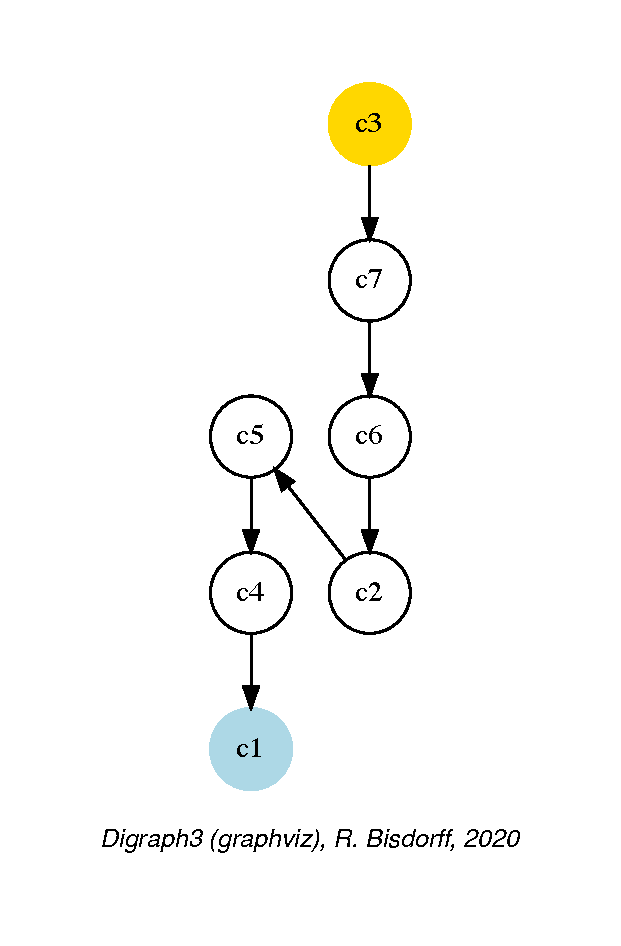
\includegraphics[width=5cm]{Figures/20-2-divGraph.pdf}
\caption{The linear ranking modelled by the majority margins digraph} 
\label{fig:20.2}       % Give a unique label
\end{figure}

\section{Bipolar approval-disapproval voting systems}
\label{sec:20.2}

Traditionally, most of the voting systems in use in the World, do only collect approval votes and abstentions, dismissing potentially strong disapproval opinions, not to be assimilated to voting abstentions. Collecting both explicit approvals ($+1$) and explicit disapprovals ($-1$) essentially enriches the expression of voters' preferences. 

In the \texttt{votingProfiles} module\index{votingProfiles@\texttt{votingProfiles} module} we provide a \texttt{BipolarApprovalVot\-ingProfile} class\index{BipolarApprovalVotingProfile@\texttt{BipolarApprovalVotingProfile} class} for handling voting results where, for each eligible Candidate \texttt{x}, the voters are invited  to \emph{approve} ($+1$), \emph{disapprove} ($-1$), or \emph{ignore} ($0$) the statement that Candidate \texttt{c} should win the election \citep{BAU-2012}.

File \texttt{bpApVotingProfile.py} contains an example of such a approval-disapproval voting profile concerning 100 voters and 15 eligible candidates \footnote{The file \texttt{bpApVotingProfile.py} may be found in the \texttt{examples} directory of the \Digraph resources.}. We can inspect its content with the \texttt{BipolarApprovalVotingProfile} class:\index{BipolarApprovalVotingProfile@\texttt{BipolarApprovalVotingProfile} class}
\begin{lstlisting}[caption={Bipolar approval voting profiles},label=list:20.9]
>>> from votingProfiles import \
...                 BipolarApprovalVotingProfile
>>> bavp = BipolarApprovalVotingProfile('bpApVotingProfile')
>>> bavp
  *------- VotingProfile instance description ------*
    Instance class   : BipolarApprovalVotingProfile
    Instance name    : bpApVotingProfile
    Candidates       : 15
    Voters           : 100
    Attributes       : ['name', 'candidates', 'voters',
                 'approvalBallot', 'netApprovalScores',
                 'ballot']
\end{lstlisting}

Beside the \texttt{candidates} and \texttt{voters} attributes, we discover in Listing~\vref{list:20.10} the \texttt{approvalBallot} attribute which gathers approval-disapproval votes. Its content is the following.
\begin{lstlisting}[caption={Inspecting an approval-disapproval ballot},label=list:20.10]
>>> bavp.approvalBallot
  {'v001':
      {'c01': Decimal('0'),
       ...
       'c04': Decimal('1'), §\label{line:20.10.5}§
       ...
       'c15': Decimal('0')
      },
   'v002':
       {'c01': Decimal('-1'), §\label{line:20.10.10}§
        'c02': Decimal('0'),
        ...
        'c15': Decimal('1')
       },
      ...
   'v100':
     {'c01': Decimal('0'),
      'c02': Decimal('1'),
      ...
      'c15': Decimal('1')
     }
    }
\end{lstlisting}	

Let us denote $A_{\mathtt{v}}$ the set of candidates approved by voter \texttt{v}. In the \texttt{approval\-Ballot} attribute we hence record in fact the bipolar-valued truth characteristic values $r(\mathtt{c} \in A_{\mathtt{v}})$ of the statements that Candidate \texttt{c} \emph{is approved} by voter \texttt{v}. In Listing~\vref{list:20.10} Line~\ref{line:20.10.5}, we observe for instance that voter \texttt{v001} positively approves Candidate \texttt{c04}. And, in Line~\ref{line:20.10.10}, we see that voter \texttt{v002} negatively approves, i.e. positively disapproves Candidate \texttt{c01}.

The \texttt{showApprovalResults()} method\index{showApprovalResults@\texttt{showApprovalResults()}} and the \texttt{showDisapproval\-Re\-sults()} method\index{showDisapprovalResults@\texttt{showDisapprovalResults()}} show how many approvals, respectively disapprovals, each candidate receives.
\begin{lstlisting}
>>> bavp.showApprovalResults()
    Approval results
     Candidate: 'c12' obtains 34 votes §\label{line:avpr.c12}§
     Candidate: 'c05' obtains 30 votes
     Candidate: 'c03' obtains 28 votes
     Candidate: 'c14' obtains 27 votes
     Candidate: 'c11' obtains 27 votes
     Candidate: 'c04' obtains 27 votes
     Candidate: 'c01' obtains 27 votes
     Candidate: 'c13' obtains 24 votes
     Candidate: 'c07' obtains 24 votes
     Candidate: 'c15' obtains 23 votes
     Candidate: 'c02' obtains 23 votes
     Candidate: 'c09' obtains 22 votes
     Candidate: 'c08' obtains 22 votes
     Candidate: 'c10' obtains 21 votes
     Candidate: 'c06' obtains 21 votes
    Total approval votes: 380
    Approval proportion: 380/1500 = 0.25
>>> bavp.showDisapprovalResults()
    Disapproval results
     Candidate: 'c12' obtains 16 votes §\label{line:davpr.c12}§
     Candidate: 'c03' obtains 22 votes
     Candidate: 'c09' obtains 23 votes
     Candidate: 'c04' obtains 24 votes
     Candidate: 'c06' obtains 24 votes
     Candidate: 'c13' obtains 24 votes
     Candidate: 'c11' obtains 25 votes
     Candidate: 'c02' obtains 26 votes
     Candidate: 'c07' obtains 26 votes
     Candidate: 'c08' obtains 26 votes
     Candidate: 'c05' obtains 27 votes
     Candidate: 'c10' obtains 27 votes
     Candidate: 'c14' obtains 27 votes
     Candidate: 'c15' obtains 27 votes
     Candidate: 'c01' obtains 32 votes
    Total disapproval votes: 376
    Disapproval proportion: 376/1500 = 0.25
\end{lstlisting}

In Lines~\ref{line:avpr.c12} and \ref{line:davpr.c12} above, we notice that, of all eligible candidates, it is Candidate \texttt{c12} who receives the highest number of approval votes (34) and the lowest number of disapproval votes (16). Total number of approval, respectively disapproval, votes approaches more or less a proportion of $25\%$ of the $100 \times 15 = 1500$ potential approval votes. About $50\%$ of the latter remain hence ignored. 

When operating now, for each Candidate \texttt{x}, the difference between the number of approval and the number of disapproval votes they receive, we obtain per candidate a corresponding \emph{net approval} score; in fact, the bipolar truth characteristic value of the statement ``\emph{Candidate} \texttt{x} \emph{should win the election}''.
\begin{equation}
r(\text{Candidate x should win the election}) \;=\; \sum_{\mathtt{v}} \big(r(\mathtt{x} \in A_{\mathtt{v}})\big)\;.
\end{equation}

These bipolar characteristic values are stored in the \texttt{netApprovalScores} attribute and may be printed out with the \texttt{showNetApprovalScores()} method\index{showNetApprovalScores@\texttt{showNetApprovalScores()}}:
\begin{lstlisting}
>>> bavp.showNetApprovalScores()
  Net Approval Scores
     Candidate: 'c12' obtains 18 net approvals §\label{line:netapsc:3}§
     Candidate: 'c03' obtains 6 net approvals
     Candidate: 'c05' obtains 3 net approvals
     Candidate: 'c04' obtains 3 net approvals
     Candidate: 'c11' obtains 2 net approvals
     Candidate: 'c14' obtains 0 net approvals
     Candidate: 'c13' obtains 0 net approvals
     Candidate: 'c09' obtains -1 net approvals
     Candidate: 'c07' obtains -2 net approvals
     Candidate: 'c06' obtains -3 net approvals
     Candidate: 'c02' obtains -3 net approvals
     Candidate: 'c15' obtains -4 net approvals
     Candidate: 'c08' obtains -4 net approvals
     Candidate: 'c01' obtains -5 net approvals
     Candidate: 'c10' obtains -6 net approvals
\end{lstlisting}

We observe in Line~\ref{line:netapsc:3} above that Candidate \texttt{c12}, with a net approval score of $34 - 16 = 18$, represents indeed the \emph{best approved} candidate for winning the election. With a net approval score of $28-22 = 6$, Candidate \texttt{c03} appears 2nd-best approved. The net approval scores define hence a potentially weak ranking on the set of eligible election candidates, and the winner(s) of the election is(are) determined by the first-ranked candidate(s).

\section{Pairwise comparison of approval-disapproval votes}
\label{sec:20.3}

The approval votes of each voter define now on the set of eligible candidates three ordered categories: his approved ($+1$), his ignored ($0$) and his disapproved ($-1$) ones. Within each of these three categories we consider the voter's actual preferences as \emph{not communicated}, i.e. as missing data. This gives for each voter a partially determined strict order which we find in the \texttt{ballot} attribute.
\begin{lstlisting}
 >>> bavp.ballot['v001']['c12']
    {'c02': Decimal('1'), 'c11': Decimal('1'),
     'c14': Decimal('1'), 'c04': Decimal('0'),
     'c06': Decimal('1'), 'c05': Decimal('1'),
     'c12': Decimal('0'), 'c13': Decimal('0'),
     'c15': Decimal('1'), 'c01': Decimal('1'),
     'c08': Decimal('1'), 'c07': Decimal('1'),
     'c09': Decimal('0'), 'c03': Decimal('1'),
     'c10': Decimal('0')}
\end{lstlisting}

For voter \texttt{v001}, for instance, the best approved Candidate \texttt{c12} is strictly preferred to Candidates: \texttt{c01}, \texttt{c02}, \texttt{c03}, \texttt{c05}, \texttt{c06}, \texttt{c07}, \texttt{c08}, \texttt{c11}, \texttt{c14} and \texttt{c15}. No candidate is preferred to \texttt{c12} and the comparison with \texttt{c04}, \texttt{c09}, \texttt{c10} and \texttt{c13} is not communicated, hence indeterminate. Mind by the way that the reflexive comparison of \texttt{c12} with itself is, as usual, ignored, i.e. indeterminate. Each voter \texttt{v} defines thus a partially determined transitive strict preference relation denoted $\succ_{\mathtt{v}}$ on the eligible candidates.

For each pair of eligible candidates, we aggregate the previous individual voter's preferences into a truth characteristic of the statement: ``Candidate $x$ is \emph{better approved than} Candidate $y$'', denoted $r(x \succ y)$:
\begin{equation}
  r(x \succ y)\;=\; \sum_{\mathtt{v}} \big(\,r(x \succ_{\mathtt{v}} y)\, \big)\;.
\end{equation}  

We say that Candidate $x$ is \emph{better approved than} Candidate $y$ when $r(x \succ y)\;>\;0$, i.e. there is a majority of voters who approve \emph{more} and disapprove \emph{less} $x$ than $y$. Vice-versa, we say that Candidate $x$ is \emph{not} better approved than Candidate $y$ when $r(x \succ y)\;<\;0$, i.e. there is a majority of voters who disapprove more and approve less $x$ than $y$. This computation is achieved with the \texttt{MajorityMarginsDigraph} constructor.
\begin{lstlisting}
>>> from votingProfiles import MajorityMarginsDigraph
>>> m = MajorityMarginsDigraph(bavp)
>>> m
  *------- Digraph instance description ------*
    Instance class      : MajorityMarginsDigraph
    Instance name       : rel_bpApVotingProfile
    Digraph Order       : 15
    Digraph Size        : 97 §\label{mmdg.8}§
    Valuation domain    : [-100.00;100.00]
    Determinateness (%) : 52.55
    Attributes          : ['name', 'actions',
               'criteria','ballot',
               'valuationdomain', 'relation',
               'order', 'gamma', 'notGamma']
\end{lstlisting}

The resulting digraph \texttt{m} contains 97 positively validated relations (see Line~\ref{mmdg.8} above) and for all pairs $(x,y)$ of eligible candidates, $r(x \succ y)$ takes value in an valuation range from $-100.00$ (unanimously rejected) to $+100.00$ (unanimously approved).

These pairwise $r(x \succ y)$ values can be inspected in a browser view with the \texttt{showHTMLRelationTable()} method: 
\begin{lstlisting}
>>> m.showHTMLRelationTable(relationName='r(x > y)')
\end{lstlisting}
\begin{figure}[ht]
%\sidecaption
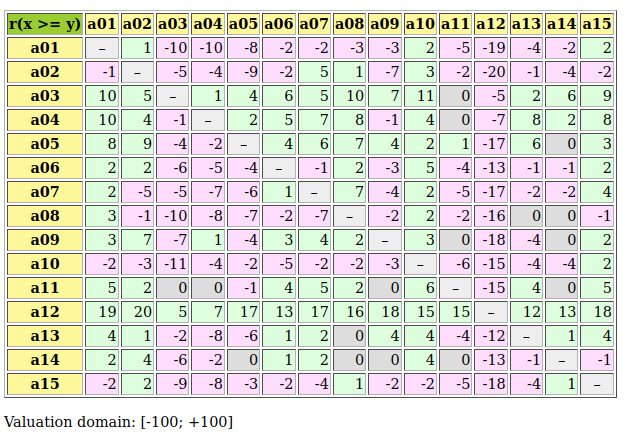
\includegraphics[width=0.8\hsize]{Figures/20-3-majMargAV.png}
\caption{The bipolar-valued pairwise majority margins} 
\label{fig:20.3}       % Give a unique label
\end{figure}

In Fig.~\vref{fig:20.3} it gets apparent that Candidate \texttt{c12} is a \Condorcet winner, i.e. the candidate who beats all the other candidates and, with the given voting profile \texttt{gavp}, should without doubt win the election. This strongly confirms the first-ranked result obtained with the previous net approval scoring. 

Let us eventually compute, with the help of the \NetFlows ranking rule\footnote{See Sect.~\ref{sec:8.3}.}, a linear ranking of the 15 eligible candidates and compare the result with the net approval scores ranking.
\begin{lstlisting}[caption={Comparing the net approval and the \NetFlows rankings},label=list:20.11]
>>> from linearOrders import NetFlowsOrder
>>> nf = NetFlowsOrder(m,Comments=True)
>>> print('NetFlows versus Net Approval Ranking')
>>> print('Candidate\tNetFlows score\tNet Approval score')
>>> for item in nf.netFlows:
...     print( '%9s\t  %+.3f\t %+.1f' %\
...	        (item[1], item[0],\
...              bavp.netApprovalScores[item[1]]) ) 
    NetFlows versus Net Approval Ranking
    Candidate	NetFlows score	Net Approval score
      'c12'	  +410.000	 +18.0
      'c03'	  +142.000	  +6.0
      'c04'	   +98.000	  +3.0
      'c05'	   +54.000	  +3.0
      'c11'	   +34.000	  +2.0
      'c09'	   -16.000	  -1.0 §\label{line:20.11.16}§
      'c14'	   -20.000	  +0.0
      'c13'	   -22.000	  +0.0
      'c06'	   -50.000	  -3.0 §\label{line:20.11.19}§
      'c07'	   -74.000	  -2.0
      'c02'	   -96.000	  -3.0
      'c08'	   -102.000	  -4.0
      'c15'	   -110.000	  -4.0
      'c10'	   -122.000	  -6.0
      'c01'	   -126.000	  -5.0
\end{lstlisting}

In Listing~\vref{list:20.11} we may notice that the \NetFlows rule delivers a ranking that is very similar to the one previously obtained with the corresponding \emph{Net Approval} scores. Only minor inversions do appear, like in the midfield, where Candidate \texttt{c09} advances before Candidates \texttt{c13} and \texttt{c14} (see Line~\ref{line:20.11.16}), and \texttt{c06} and \texttt{c07} swap their positions 9 and 10 (see Line~\ref{line:20.11.19}). The two last-ranked Candidates \texttt{c10} and \texttt{c01} also swap their positions.

This confirms again the pertinence of the net approval scoring approach for finding the winner in an approval-disapproval voting system. Yet, voting by approving ($+1$), disapproving ($-1$) or ignoring ($0$) eligible candidates, may also be seen as a performance evaluation of the eligible candidates on a $\{-1, 0, 1\}$-valued ordinal scale.

\section{Three-valued evaluative voting systems}
\label{sec:20.4}

Following such an epistemic perspective, we may effectively convert the given \texttt{BipolarApprovalVotingProfile} instance into a \texttt{PerformanceTableau} instance, so as to get access to a corresponding outranking decision aiding approach.

Mind that, contrary to the majority margins of the ``\emph{better approved than}'' relation, all voters consider now the approved candidates to be equivalent ($+1$). Same is true for the disapproved ($-1$), respectively the ignored ($0$) candidates. The voter's marginal preferences model this time a complete preorder with three equivalence classes. 

From the saved file \texttt{AVPerfTab.py} (see Line~\ref{line:20.12.1} below), we may construct an outranking relation on the eligible candidates with our standard \texttt{BipolarOutran\-kingDigraph} class constructor. The semantics of this outranking relation are the following:
\begin{itemize}[nosep,leftmargin=0.5cm,rightmargin=0.5cm]
\item We say that Candidate $x$ \emph{outranks} Candidate $y$ when there is a majority of voters who consider $x$ \emph{at least as well evaluated as} $y$;
\item We say that Candidate $x$ is \emph{outranked by} Candidate $y$ when there is a majority of voters who consider $x$ \emph{not at least as well evaluated as} $y$;
\item Otherwise, the outranking situation is indeterminate.
\end{itemize}
\begin{lstlisting}[caption={Computing the outranking digraph},label=list:20.12]
>>> bavp.save2PerfTab(fileName='AVPerfTab',valueDigits=0) §\label{line:20.12.1}§
  *--- Saving as performance tableau in AVPerfTab.py ---*
>>> from outrankingDigraphs import\
...                         BipolarOutrankingDigraph
>>> odg = BipolarOutrankingDigraph('AVPerfTab')
>>> odg
  *------- Object instance description ------*
    Instance class       : BipolarOutrankingDigraph
    Instance name        : rel_AVPerfTab
    Actions              : 15
    Criteria             : 100
    Size                 : 210 §\label{line:20.12.12}§
    Determinateness (%)  : 69.29
    Valuation domain     : [-1.00;1.00]
    Attributes           : ['name', 'actions', 'order,
                       'criteria', 'evaluation', 'NA',
                       'valuationdomain', 'relation',
                       'gamma', 'notGamma', ...]
\end{lstlisting}

The size ($210 = 15 \times 14$) of the resulting outranking digraph \texttt{odg}, shown in Listing~\vref{list:20.12} Line~\ref{line:20.12.12} above, reveals that the corresponding ``\emph{at least as good evaluated as}'' relation models actually a trivial \emph{complete} digraph. All candidates appear to be \emph{equally} at least as well evaluated and the strict ``\emph{better evaluated than}'' (codual) outranking digraph becomes in fact empty. The converted performance tableau does apparently not contain sufficiently discriminatory performance evaluations for supporting any strict preference situations.

Yet, we may nevertheless try to apply again the \NetFlows ranking rule to this complete outranking digraph \texttt{odg} and print side by side the corresponding \NetFlows scores and the previous Net Approval scores. 
\begin{lstlisting}[caption={Comparing the \NetFlows and the Net Approval rankings},label=list:20.13]
>>> from linearOrders import NetFlowsOrder
>>> nf = NetFlowsOrder(odg)
>>> print('NetFlows versus Net Approval Ranking')
>>> print('Candidate\tNetFlows Score\tNet Approval Score')
>>> for item in nf.netFlows:
...     print('%9s\t  %+.3f\t %+.0f' %\
...         (item[1],item[0],\
...          bavp.netApprovalScores[item[1]]) )  
    NetFlows versus Net Approval Ranking
    Candidate    NetFlows score	Net Approval score
      c12	  +4.100	    +18
      c03	  +1.420	     +6
      c04	  +0.980	     +3
      c05	  +0.540             +3
      c11	  +0.340	     +2
      c09	  -0.160	     -1
      c14	  -0.200	      0
      c13	  -0.220	      0
      c06	  -0.500	     -3
      c07	  -0.740	     -2
      c02	  -0.960	     -3
      c08	  -1.020	     -4
      c15	  -1.100	     -4
      c10	  -1.220	     -6
      c01	  -1.260	     -5
\end{lstlisting}

Despite its apparent poor strict preference discriminating power, we obtain in Listing~\vref{list:20.13} here \NetFlows scores that are directly proportional (divided by $100$) to the scores obtained with the \emph{better approved than} majority margins digraph \texttt{m} (see List.~\vref{list:20.11}).

Encouraged by this positive result, we may furthermore compute a \Rubis best choice recommendation (see Chap.~\ref{sec:4}).
\begin{lstlisting}[caption={Computing a best social choice recommendation},label=list:20.14]
>>> odg.showBestChoiceRecommendation()
  Rubis best choice recommendation(s) (BCR)
   (in decreasing order of determinateness)   
   Credibility domain: [-1.00,1.00]
  === >> ambiguous first choice(s) 
   * choice        : ['c01','c02','c03','c04','c05', §\label{line:20.14.6}§
                      'c06','c07','c08','c09','c10',
                      'c11','c12','c13','c14','c15'] §\label{line:20.14.8}§
    independence   : 0.06
    dominance      : 1.00
    absorbency     : 1.00
    covering (%)   : 100.00
    determinateness (%) : 61.13
    - most credible action(s) = {
        'c12': 0.44, 'c03': 0.34, 'c04': 0.30, §\label{line:20.14.15}§
        'c14': 0.28, 'c13': 0.24, 'c06': 0.24,
        'c11': 0.20, 'c10': 0.20, 'c07': 0.20,
        'c01': 0.20, 'c08': 0.18, 'c05': 0.18,
        'c15': 0.14, 'c09': 0.14, 'c02': 0.06, }
   === >> ambiguous last choice(s)
    * choice        : ['c01','c02','c03','c04','c05',
                      'c06','c07','c08','c09','c10',
                      'c11','c12','c13','c14','c15']
     independence   : 0.06
     dominance      : 1.00
     absorbency     : 1.00
     covered (%)    : 100.00
     determinateness (%) : 63.73
     - most credible action(s) = {
         'c13': 0.36, 'c06': 0.36, 'c15': 0.34, §\label{line:20.14.30}§
         'c01': 0.34, 'c08': 0.32, 'c07': 0.30,
         'c02': 0.30, 'c14': 0.28, 'c11': 0.28,
         'c09': 0.28, 'c04': 0.26, 'c10': 0.24,
         'c05': 0.20, 'c03': 0.20, 'c12': 0.06, }
\end{lstlisting}

The strict outranking digraph $(\sim (-odg))$ being actually $empty$, we obtain a unique \emph{ambiguous} --first as well as last-- choice recommendation which trivially retains all fifteen candidates (see List.~\vref{list:20.14} Lines~\ref{line:20.14.6}-\ref{line:20.14.8} above). Yet, the bipolar-valued best choice membership characteristic vector reveals that, among all the fifteen potential winners, it is indeed Candidate \texttt{c12} the most credible one with a $72\%$ majority of voters' support (see Line~\ref{line:20.14.15}, $(0.44 + 1.0)/2\;=\; 0.72$); followed by Candidate \texttt{c03} ($67\%$) and Candidate \texttt{c04} ($65\%$). Similarly, Candidates \texttt{c13} and \texttt{c06} represent the most credible losers with a $68\%$ majority voters' support (Line~\ref{line:20.14.30}).

We observe here empirically that \emph{evaluative} voting systems, using three-valued ordinal performance scales, match closely corresponding approval-disapproval voting systems. The latter systems model, however, more faithfully the very preferential information that is expressed with \emph{approved}, \emph{disapproved} and \emph{ignored} statements. The corresponding evaluation on a three-level scale, being value (numbers) based, cannot express the fact that in approval-disapproval voting system there is no preferential information given concerning the pairwise comparison of all approved, respectively disapproved or ignored candidates.

Let us finally illustrate how approval-disapproval voting systems may favour multipartisan supported candidates. We shall therefore compare \emph{approval-disapproval} versus \emph{uninominal plurality} election results when considering a highly divisive and partisan political context.
 
\section{Favouring multipartisan candidates}
\label{sec:20.5}

In modern democracy, politics  are largely structured by political parties and activists. Let us so consider an approval-disapproval voting profile \texttt{dvp} where the random voter behaviour is simulated from two pre-electoral polls concerning a political scene with essentially two major highly competing parties, like the one existing in the US.
\begin{lstlisting}[caption={A random approval-disapproval voting profile in a divisive political context},label=list:20.15]
>>> dvp = RandomBipolarApprovalVotingProfile(\
...                numberOfCandidates=15,\
...                numberOfVoters=100,
...                approvalProbability=0.25,
...                disapprovalProbability=0.25,
...                WithPolls=True,
...                partyRepartition=0.5,
...                other=0.05,
...                DivisivePolitics=True,
...                seed=200)
>>> dvp.showRandomPolls()
  Random repartition of voters
  Party-1 supporters : 45 (45.00%)
  Party-2 supporters : 49 (49.00%)
  Other voters       : 6 (06.00%)
  *---------------- random polls -----------------
  Party-1(45.0%) | Party-2(49.0%) |   expected  
  ------------------------------------------------
  'c05' : 24.10% | 'c07' : 24.10% | 'c07' : 11.87%
  'c14' : 23.48% | 'c10' : 23.48% | 'c10' : 11.60%
  'c03' : 15.13% | 'c01' : 15.13% | 'c05' : 10.91%
  'c12' : 07.55% | 'c04' : 07.55% | 'c14' : 10.67%
  'c08' : 07.11% | 'c09' : 07.11% | 'c01' : 07.67%
  'c15' : 04.37% | 'c13' : 04.37% | 'c03' : 07.09%
  'c11' : 03.99% | 'c02' : 03.99% | 'c04' : 04.55%
  'c06' : 03.80% | 'c06' : 03.80% | 'c09' : 04.49%
  'c02' : 02.79% | 'c11' : 02.79% | 'c12' : 04.32%
  'c13' : 02.63% | 'c15' : 02.63% | 'c08' : 04.30%
  'c09' : 02.24% | 'c08' : 02.24% | 'c06' : 03.57%
  'c04' : 01.89% | 'c12' : 01.89% | 'c13' : 03.32%
  'c01' : 00.57% | 'c03' : 00.57% | 'c15' : 03.25%
  'c10' : 00.20% | 'c14' : 00.20% | 'c02' : 03.21%
  'c07' : 00.14% | 'c05' : 00.14% | 'c11' : 03.16%
\end{lstlisting}   

In Listing~\vref{list:20.15}, the divisive political situation is reflected by the fact that Party-1 and Party-2 supporters show strict opposite preferences. The leading candidates of Party-1 (\texttt{c05} and \texttt{c14}) are last choices for Party-2 supporters and, Candidates \texttt{c07} and \texttt{c10}, leading candidates for Party-2 supporters, are similarly the least choices for Party-1 supporters.

No clear winner may be guessed from these pre-election polls. As Party-2 shows however slightly more supporters than Party-1, the expected winner in an uninominal plurality or instant-run-off voting system will be Candidate \texttt{c07}, i,e, the leading candidate of majority Party-2 (see below).
\begin{lstlisting}
>>> dvp.computeSimpleMajorityWinner()
  ['c07']
>>> dvp.computeInstantRunoffWinner()
  ['c07']
\end{lstlisting}

Now, in a corresponding approval-disapproval voting system, Party-1 supporters will usually approve their leading candidates and disapprove the leading candidates of Party-2. Vice versa, Party-2 supporters will usually approve their leading candidates and disapprove the leading candidates of Party-1. Let us consult the resulting approval votes per candidate.
\begin{lstlisting}
>>> dvp.showApprovalResults()
     Candidate: 'c07' obtains 30 votes
     Candidate: 'c10' obtains 28 votes
     Candidate: 'c05' obtains 28 votes
     Candidate: 'c01' obtains 28 votes
     Candidate: 'c03' obtains 26 votes
     Candidate: 'c02' obtains 26 votes
     Candidate: 'c12' obtains 25 votes
     Candidate: 'c14' obtains 24 votes
     Candidate: 'c13' obtains 24 votes
     Candidate: 'c09' obtains 21 votes
     Candidate: 'c04' obtains 21 votes
     Candidate: 'c08' obtains 19 votes
     Candidate: 'c06' obtains 17 votes
     Candidate: 'c15' obtains 15 votes
     Candidate: 'c11' obtains 12 votes
    Total approval votes: 344
    Approval proportion: 344/1500 = 0.23
\end{lstlisting}

When considering only the approval votes, we find confirmed above that the leading candidate of Party-2 obtains in this simulation a plurality of approval votes. In uninominal plurality or instant-runoff voting systems, this candidate wins hence the election, quite to the despair of Party-1 supporters. As a foreseeable consequence, this election result will be more or less aggressively contested which leads to a loss of popular trust in democratic elections and institutions.

If we look however on the corresponding disapprovals, we discover that, not surprisingly, the leading candidates of both parties collect by far the highest number of disapproval votes. 
\begin{lstlisting}
>>> dvp.showDisapprovalResults()
     Candidate: 'c02' obtains 14 votes
     Candidate: 'c04' obtains 14 votes
     Candidate: 'c13' obtains 14 votes
     Candidate: 'c06' obtains 15 votes
     Candidate: 'c09' obtains 15 votes
     Candidate: 'c08' obtains 16 votes
     Candidate: 'c11' obtains 16 votes
     Candidate: 'c15' obtains 18 votes
     Candidate: 'c12' obtains 20 votes
     Candidate: 'c01' obtains 29 votes
     Candidate: 'c03' obtains 30 votes
     Candidate: 'c10' obtains 37 votes
     Candidate: 'c07' obtains 44 votes
     Candidate: 'c14' obtains 45 votes
     Candidate: 'c05' obtains 49 votes
    Total disapproval votes: 376
    Disapproval proportion: 376/1500 = 0.25
\end{lstlisting}

Balancing now approval against disapproval votes will favour the moderate, bipartisan supported, candidates.
\begin{lstlisting}
>>> dvp.showNetApprovalScores()
    Net Approval Scores
     Candidate: 'c02' obtains 12 net approvals
     Candidate: 'c13' obtains 10 net approvals
     Candidate: 'c04' obtains 7 net approvals
     Candidate: 'c09' obtains 6 net approvals
     Candidate: 'c12' obtains 5 net approvals
     Candidate: 'c08' obtains 3 net approvals
     Candidate: 'c06' obtains 2 net approvals
     Candidate: 'c01' obtains -1 net approvals
     Candidate: 'c15' obtains -3 net approvals
     Candidate: 'c11' obtains -4 net approvals
     Candidate: 'c03' obtains -4 net approvals
     Candidate: 'c10' obtains -9 net approvals
     Candidate: 'c07' obtains -14 net approvals
     Candidate: 'c14' obtains -21 net approvals
     Candidate: 'c05' obtains -21 net approvals
\end{lstlisting}

Candidate \texttt{c02}, appearing in the pre-electoral polls in the midfield (in position 7 for Party-2 and in position 9 for Party-1 supporters, see List.\vref{list:20.15}), shows indeed the highest net approval score. Second highest net approval score obtains Candidate \texttt{c13}, in  position 6 for Party-2 and in position 10 for Party-1 supporters.

Figure~\vref{fig:20.4}, showing the \NetFlows ranked relation table of the ``\emph{better approved than}'' majority margins digraph, confirms below this net approval scoring result.
\begin{lstlisting}
>>> m = MajorityMarginsDigraph(dvp)
>>> m.showHTMLRelationTable(\
...      actionsList=m.computeNetFlowsRanking(),
...      relationName='r(x > y)')
\end{lstlisting}	   
\begin{figure}[ht]
%\sidecaption
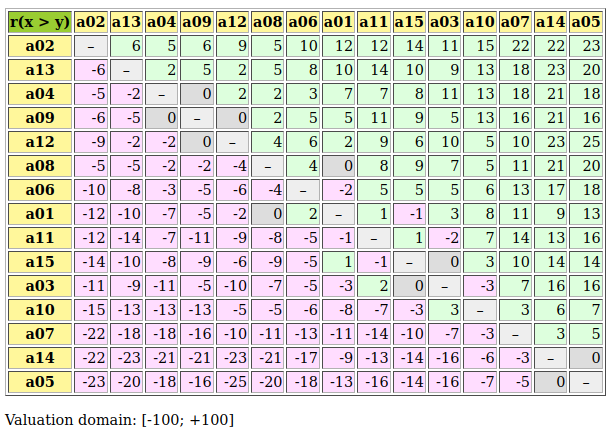
\includegraphics[width=0.8\hsize]{Figures/20-4-majMargDAV.png}
\caption{The pairwise \emph{better approved than} majority margins} 
\label{fig:20.4}       % Give a unique label
\end{figure}

Candidate \texttt{c02} appears indeed \emph{better approved than} any other candidate (\Condorcet winner); and, the leading Candidates of Party-1, \texttt{c05} and \texttt{c14}, are \emph{less approved than} any other candidates (weak \Condorcet losers).
\begin{lstlisting}
>>> m.computeCondorcetWinners()
  ['c02']
>>> m.computeWeakCondorcetLosers()
  ['c05','c14']
\end{lstlisting}

We see this result furthermore confirmed when computing the corresponding first, respectively last choice recommendation.    
\begin{lstlisting}
>>> m.showBestChoiceRecommendation()
  Rubis best choice recommendation(s) (BCR)
   (in decreasing order of determinateness)   
   Credibility domain: [-100.00,100.00]
   === >> potential first choice(s)
    * choice              : ['c02']
      independence        : 100.00
      dominance           : 5.00
      absorbency          : -23.00
      covering (%)        : 100.00
      determinateness (%) : 52.50
      - most credible action(s) = { 'c02': 5.00, }
   === >> potential last choice(s) 
    * choice              : ['c05', 'c14']
      independence        : 0.00
      dominance           : -23.00
      absorbency          : 5.00
      covered (%)         : 100.00
      determinateness (%) : 50.00
      - most credible action(s) = { }
\end{lstlisting}

Candidate \texttt{c02}, being actually a \Condorcet winner, gives an initial prekernel of digraph \texttt{m}, whereas Party-1 leading Candidates \texttt{c05} and \texttt{c14}, both being weak \Condorcet losers, give together a terminal prekernel. They hence represent our \emph{first choice}, respectively, \emph{last choice} recommendations for winning this simulated election.

It is worthwhile noticing again the essential structural and computational role, the ignored value is playing in approval-disapproval voting systems. This epistemic and logical \emph{neutral} term is needed indeed for handling in a consistent and efficient manner \emph{not communicated votes} and/or \emph{indeterminate} preferential statements.

Let us conclude by predicting that, for leading political candidates in an aggressively divisive political context, the perspective to easily fail election withan approval-disapproval voting system, might or will induce a change in the usual way of running electoral campaigns. Political parties and politicians, who avoid aggressive competitive propaganda and instead propose multipartisan collaborative social choices, will be rewarded with better election results than any kind of extremism. It could mean the end of sterile political obstructions and war like electoral battles. \emph{Let's do it !}.

\vspace{\baselineskip}
The last Part V of this monograph illustrates in three chapters computational resources for working with simple undirected graphs.

%%%%%%% The chapter bibliography
%\normallatexbib
%\clearpage
%\phantomsection
%\addcontentsline{toc}{section}{Chapter Bibliography}
\chapter{Tempering plurality tyranny effects in social choice}
\label{sec:20}


\abstract*{ In a \emph{social choice} context, where decision objectives would match different political parties, Pareto efficient choice recommendations represent in fact \emph{multipartisan} social choices that may judiciously deliver the primary selection in a two stage election system. Our bipolar-valued outranking model is based on approvals-disapprovals of ``\emph{at least as well evaluated as}'' statements. A similar approach is put into practice with approval-disapproval voting systems. When converting such approval-disapproval voting ballots into corresponding performance records, we obtain a $(-1,0,1)$-valued evaluative voting system. We eventually show that in such a approval-disapproval voting system, the winner tends to be among the more or less multipartisan candidates.}

\begin{quotation}\emph{The choice of a voting procedure shapes the democracy in which we live}.\\
    -- \citet*{BAU-2012}.
\end{quotation}
\vspace{1cm}

\abstract{ In a \emph{social choice} context, where decision objectives would match different political parties, Pareto efficient choice recommendations represent in fact \emph{multipartisan} social choices that may judiciously deliver the primary selection in a two stage election system. Our bipolar-valued outranking model is based on approvals-disapprovals of ``\emph{at least as well evaluated as}'' statements. A similar approach is put into practice with approval-disapproval voting systems. When converting such approval-disapproval voting ballots into corresponding performance records, we obtain a $(-1,0,1)$-valued evaluative voting system. We eventually show that in such a approval-disapproval voting system, the winner tends to be among the more or less multipartisan candidates.}

\paragraph{\textbf{Introduction}}

From the seminal work by \emph{Bernard Roy}\index{Roy@\textsl{B. Roy}} on, tempering plurality tyranny effects is achieved in the outranking approach by taking into account considerable negative performance differences that render doubtful otherwise positive ``\emph{at least as well evaluated as}'' situations \citep*{ROY-1966}. In the social choice context of general elections, such a polarisation is not feasible as the genuine uninominal voting ballots do not contain a rich enough preferential information. Yet, when matching decision objectives with political parties, the Pareto efficient outranking situations seen in Sect.~\ref{sec:19.6}, correspond to multipartisan ``\emph{at least as well approved as}'' situations when pairwisely comparing the eligible candidates. A best choice recommendation based of the corresponding multipartisan strict ``\emph{better approved as}'' situations may, the case given, deliver a convincing primary selection in a two-stage election. 

\section{Two-stage elections with multipartisan primary selection}
\label{sec:20.1}

To compute multipartisan social choices we need to, first, convert a given linear voting profile with pre-election polls into a corresponding performance tableau. We shall illustrate this point with a voting profile we discussed already in Chap.~\ref{sec:7}.
\begin{lstlisting}[caption={Example of a 3 parties voting profile},label=list:20.1]
>>> from votingProfiles import RandomLinearVotingProfile
>>> lvp = RandomLinearVotingProfile(numberOfCandidates=15,
...                         numberOfVoters=1000,
...                         WithPolls=True,
...                         partyRepartition=0.5,
...                         other=0.1,
...                         seed=0.9189670954954139)
>>> lvp
  *------- VotingProfile instance description ------*
   Instance class   : RandomLinearVotingProfile
   Instance name    : randLinearProfile
   Candidates       : 15
   Voters           : 1000
   Attributes       : ['name', 'seed', 'candidates',
             'voters', 'WithPolls', 'RandomWeights',
             'sumWeights', 'poll1', 'poll2',
             'other', partyRepartition,
             'linearBallot', 'ballot']
>>> lvp.showRandomPolls() §\label{line:20.1.20}§
  Random repartition of voters
   Party_1 supporters : 460 (46.0%)
   Party_2 supporters : 436 (43.6%)
   Other voters       : 104 (10.4%)
  *---------------- random polls ----------------
   Party-1(46.0%) | Party-(43.6%)|  expected  
   ----------------------------------------------
    c06 : 19.91%  | c11 : 22.94%  | c06 : 15.00%
    c07 : 14.27%  | c08 : 15.65%  | c11 : 13.08%
    c03 : 10.02%  | c04 : 15.07%  | c08 : 09.01%
    c13 : 08.39%  | c06 : 13.40%  | c07 : 08.79%
    c15 : 08.39%  | c03 : 06.49%  | c03 : 07.44%
    c11 : 06.70%  | c09 : 05.63%  | c04 : 07.11%
    c01 : 06.17%  | c07 : 05.10%  | c01 : 05.06%
    c12 : 04.81%  | c01 : 05.09%  | c13 : 05.04%
    c08 : 04.75%  | c12 : 03.43%  | c15 : 04.23%
    c10 : 04.66%  | c13 : 02.71%  | c12 : 03.71%
    c14 : 04.42%  | c14 : 02.70%  | c14 : 03.21%
    c05 : 04.01%  | c15 : 00.86%  | c09 : 03.10%
    c09 : 01.40%  | c10 : 00.44%  | c10 : 02.34%
    c04 : 01.18%  | c05 : 00.29%  | c05 : 01.97%
    c02 : 00.90%  | c02 : 00.21%  | c02 : 00.51% §\label{line:20.1.end}§
\end{lstlisting}

In this example (see List.~\vref{list:20.1} Lines~\ref{line:20.1.20}-\ref{line:20.1.end}), we observe 460 Party-1 supporters ($46\%$), 436 Party-2 supporters ($43.6\%$) and 104 other voters ($10.4\%$). Favorite candidates of Party-1 supporters, with more than $10\%$, are \texttt{c06} ($19.91\%$), \texttt{c07} ($14.27\%$) and \texttt{c03} ($10.02\%$). Whereas for Party-2 supporters, favorite candidates are \texttt{c11} ($22.94\%$), followed by \texttt{c08} ($15.65\%$), \texttt{c04} ($15.07\%$) and \texttt{c06} ($13.4\%$).

We can convert this linear voting profile into a \texttt{PerformanceTableau} object where each political party matches a decision objective.
\begin{lstlisting}[caption={Converting a voting profile into a performance tableau},label=list:20.2]
>>> lvp.save2PerfTab('votingPerfTab')§\label{line:20.2.1}§
>>> from perfTabs import PerformanceTableau
>>> vpt = PerformanceTableau('votingPerfTab')§\label{line:20.2.3}§
>>> vpt
  *------- PerformanceTableau instance description ---*
    Instance class   : PerformanceTableau
    Instance name    : votingPerfTab
    Actions          : 15
    Objectives       : 3
    Criteria         : 1000
    Attributes       : ['name', 'actions', 'objectives',
              'criteria', 'weightPreorder', 'evaluation']
>>> vpt.objectives
  OrderedDict([
    ('party0', {'name': 'other', 'weight': Decimal('104'),
     'criteria': ['v0003', 'v0008', 'v0011', ... ']}),
    ('party1', {'name': 'party 1', 'weight': Decimal('460'),
     'criteria': ['v0002', 'v0006', 'v0007', ...]}),
    ('party2', {'name': 'party 2', 'weight': Decimal('436'),
      'criteria': ['v0001', 'v0004', 'v0005', ... ]})
    ])
\end{lstlisting}

In Listing~\vref{list:20.2} the linear voting profile lvp is first stored in \texttt{Performance\-Tableau} format (see Line~\ref{line:20.2.1}). In Line~\ref{line:20.2.3}, the PerformanceTableau class reloads this stored performance tableau data. The three parties of the linear voting profile represent three decision objectives and the 1000 voters are distributed as 1000 performance criteria according to the party they support.

In order to operate now a \emph{primary multipartisan selection} of potential election winners, we compute the corresponding unopposed multiobjective outranking digraph (see Sect.~\ref{sec:19.5}).
\begin{lstlisting}[caption={Computing unopposed multiobjective outranking situations},label=list:20.3]
>>> from outrankingDigraphs import \
...       UnOpposedBipolarOutrankingDigraph
>>> uog = UnOpposedBipolarOutrankingDigraph(vpt)
>>> uog
  *------- Object instance description ------*
    Instance class      : UnOpposedBipolarOutrankingDigraph
    Instance name       : unopposed_outrankings
    Actions             : 15
    Criteria            : 1000
    Size                : 34
    Oppositeness (%)    : 67.31 §\label{line:20.3.opp}§
    Determinateness (%) : 57.61
    Valuation domain    : [-1.00;1.00]
    Attributes          : ['name', 'actions', 'valuationdomain',
                           'objectives', 'criteria', 'methodData',
                           'evaluation', 'order', 'runTimes',
                           'relation', 'marginalRelationsRelations',
                           'gamma', 'notGamma']
\end{lstlisting}

From the potential 105 pairwise outranking situations, we keep 34 positively validated outranking situations, leading to a degree of \emph{oppositeness} between political parties of $67.31\%$ (see List.~\ref{list:20.3} Line~\ref{line:20.3.opp}).

The corresponding bipolar-valued relation table can be shown by orienting the list of candidates with the help of the initial and terminal prekernels.\index{showPreKernels@\texttt{showPreKernels()}}
\begin{lstlisting}[caption={Computing unopposed multiobjective outranking situations},label=list:20.4]
>>> uog.showPreKernels()
  *--- Computing preKernels ---*
   Dominant preKernels :
    ['c11', 'c06', 'c13', 'c15']
       independence :  0.0
       dominance    :  0.18
       absorbency   :  -0.66
       covering     :  0.43
   Absorbent preKernels :
    ['c02', 'c04', 'c14', 'c03']
       independence :  0.0
       dominance    :  0.0
       absorbency   :  0.37
       covered      :  0.46
>>> orientedCandidatesList = ['c06','c11','c13','c15',\
...         'c01','c05','c07','c08','c09','c10','c12',\
...         'c02','c03','c04','c14']
>>> uog.showHTMLRelationTable(\
...    actionsList=orientedCandidatesList,\
...    tableTitle='Unopposed three-partisan outrankings')
\end{lstlisting}

\begin{figure}[ht]
%\sidecaption
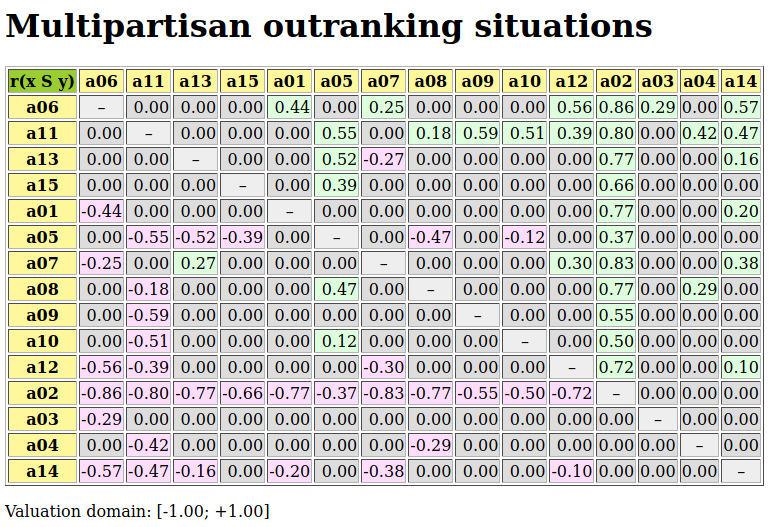
\includegraphics[width=0.9\hsize]{Figures/20-1-unOpposedOutrankings.png}
\caption{Relation table of multipartisan outranking digraph} 
\label{fig:20.1}       % Give a unique label
\end{figure}

In Fig.~\vref{fig:20.1}, we may notice that the dominating outranking prekernel \{\texttt{c06}, \texttt{c11}, \texttt{c13}, \texttt{c15}\} gathers in fact a multipartisan selection of potential election winners. It is worthwhile noticing that the majority margins obtained from a linear voting profile do verify the zero-sum rule: $\big(\,r(x \succsim y) \,+\, r(y \succsim x) \;=\; 0.0\,\big)$. To each positive outranking situation corresponds an equivalent negative converse situation and the resulting outranking and strict outranking digraphs are the same.

When restricting now, in a secondary election stage, the set of eligible candidates to this dominating prekernel, we may compute the actual best social choice.
\begin{lstlisting}[caption={Recommending the secondary election winner},label=list:20.5]
>>> from outrankingDigraphs import BipolarOutrankingDigraph
>>> g2 = BipolarOutrankingDigraph(vpt,\
..          actionsSubset=['c06','c11','c13','c15'])
>>> g2.showRelationTable(ReflexiveTerms=False)
  * ---- Relation Table -----
     r    | 'c06'  'c11'  'c13'  'c15'   
    ------|----------------------------
    'c06' |   -    +0.10  +0.48  +0.52  §\label{line:20.5.8}§
    'c11' | -0.10    -    +0.27  +0.29  
    'c13' | -0.48  -0.27    -    +0.19  
    'c15' | -0.52  -0.29  -0.19    -    §\label{line:20.5.11}§
    Valuation domain: [-1.0; 1.0]
>>> g2.computeCondorcetWinners()
  ['c06']
>>> g2.computeCopelandRanking()
  ['c06', 'c11', 'c13', 'c15']
\end{lstlisting}

Candidate \texttt{c06} appears clearly to be the winner of this election. Notice by the way that the restricted pairwise outranking relation, shown in Listing~\ref{list:20.5} Lines~\ref{line:20.5.8}-\ref{line:20.5.11}, models a linear ordering of the preselected candidates.

We can eventually check the quality of this best choice by noticing that Candidate \texttt{c06} represents indeed the \emph{simple majority}, the \emph{instant runoff}, the \Borda, as well as the \Condorcet winner of the initially given linear voting profile \texttt{lvp}.
\begin{lstlisting}
>>> lvp.computeSimpleMajorityWinner()
  ['c06']
>>> lvp.computeInstantRunoffWinner()
  ['c06']
>>> lvp.computeBordaWinners()
  ['c06']
>>> from votingProfiles import MajorityMarginsDigraph
>>> cd = MajorityMarginsDigraph(lvp)
>>> cd.computeCondorcetWinners()
  ['c06']
\end{lstlisting}

In our example voting profile here, the multipartisan primary selection stage appears quite effective in reducing the number of eligible candidates to four out of a set of 15 candidates without by the way rejecting the actual winning candidate.

However, in a very \emph{divisive} two major parties system, like in the US, where preferences of the supporters of one major party are opposite to the preferences of the supporters of the other major party, the multipartisan outranking digraph will become nearly indeterminate.

In Listing~\vref{list:20.6} below we generate such a divisive kind of linear voting profile with the help of the \texttt{DivisivePolitics} flag (see Lines~\ref{line:20.6.4} and \ref{line:20.6.14}-\ref{line:20.6.20}). When now converting the voting profile into a performance tableau (Lines 20-21), we can compute the corresponding unopposed outranking digraph.
\begin{lstlisting}[caption={A divisive two-party example of a random linear voting profile},label=list:20.6]
>>> from votingProfiles import RandomLinearVotingProfile		     
>>> lvp = RandomLinearVotingProfile(\
...      numberOfCandidates=7,numberOfVoters=500,\
...      WithPolls=True, partyRepartition=0.4,other=0.2,\ §\label{line:20.6.4}§
...      DivisivePolitics=True, seed=1)
>>> lvp.showRandomPolls()
  Random repartition of voters
   Party-1 supporters : 240 (48.00%)
   Party-2 supporters : 160 (32.00%)
   Other voters       : 100 (20.00%)
  *---------------- random polls -------------
   Party_1(48.0%) | Party_2(32.0%) | expected  
   -------------------------------------------
   c2 : 30.84%    |  c1 : 30.84%   | c2 : 15.56% §\label{line:20.6.14}§
   c3 : 23.67%    |  c4 : 23.67%   | c3 : 12.91%
   c7 : 17.29%    |  c6 : 17.29%   | c7 : 11.43%
   c5 : 11.22%    |  c5 : 11.22%   | c1 : 11.00%
   c6 : 09.79%    |  c7 : 09.79%   | c6 : 10.23%
   c4 : 04.83%    |  c3 : 04.83%   | c4 : 09.89%
   c1 : 02.37%    |  c2 : 02.37%   | c5 : 08.98% §\label{line:20.6.20}§
>>> lvp.save2PerfTab('divisiveExample')
>>> dvp = PerformanceTableau('divisiveExample')
>>> from outrankingDigraphs import \
...        UnOpposedBipolarOutrankingDigraph
>>> uodg = UnOpposedBipolarOutrankingDigraph(dvp)
>>> uodg
  *------- Object instance description ------*
   Instance class : UnOpposedBipolarOutrankingDigraph
   Instance name  : divisiveExample
   Actions        : 7
   Criteria       : 500
   Size           : 0 §\label{line:20.6.32}§
   Oppositeness (%)    : 100.00 §\label{line:20.6.33}§
   Determinateness (%) : 50.00
   Valuation domain    : [-1.00;1.00]
\end{lstlisting}

With an oppositeness degree of $100.0\%$ (see List.~\vref{list:20.6} Lines~\ref{line:20.6.32}-\ref{line:20.6.33}), the preferential disagreement between the political parties is complete, and the unopposed outranking digraph \texttt{uodg} becomes completely indeterminate as shown in the relation table below.
\begin{lstlisting}
>>> uodg.showRelationTable(ReflexiveTerms=False)
  * ---- Relation Table -----
   r   | 'c1'   'c2'  'c3'  'c4'  'c5'  'c6'  'c7'   
  -----|------------------------------------------
  'c1' |   -   +0.00 +0.00 +0.00 +0.00 +0.00 +0.00  
  'c2' | +0.00   -   +0.00 +0.00 +0.00 +0.00 +0.00  
  'c3' | +0.00 +0.00   -   +0.00 +0.00 +0.00 +0.00  
  'c4' | +0.00 +0.00 +0.00   -   +0.00 +0.00 +0.00  
  'c5' | +0.00 +0.00 +0.00 +0.00   -   +0.00 +0.00  
  'c6' | +0.00 +0.00 +0.00 +0.00 +0.00   -   +0.00  
  'c7' | +0.00 +0.00 +0.00 +0.00 +0.00 +0.00   -   
  Valuation domain: [-1.0; 1.0]
\end{lstlisting}      

As a consequence, a multipartisan primary selection, computed with a \texttt{show\-Best\-ChoiceRecommendation()} method,  will keep the complete initial set of eligible candidates and, hence, become \emph{ineffective} (see List.~\vref{list:20.7} Line~\ref{line:20.7.6}).
\begin{lstlisting}[caption={Example of ineffective primary multipartisan selection},label=list:20.7]
>>> uodg.showBestChoiceRecommendation()
  Rubis best choice recommendation(s) (BCR)
   (in decreasing order of determinateness)   
   Credibility domain: [-1.00,1.00]
   === >> ambiguous choice(s)
    choice              : ['c1','c2','c3','c4','c5','c6','c7'] §\label{line:20.7.6}§
    independence        : 0.00
    dominance           : 1.00
    absorbency          : 1.00
    covered (%)         : 100.00
    determinateness (%) : 50.00
     - most credible action(s) = { }
\end{lstlisting}

With such kind of divisive voting profile, there may indeed not always exist an obvious winner. In Listing~\vref{list:20.8}, we see, for instance, that the simple majority winner is \texttt{c2} (Line~\ref{line:20.8.2}), whereas the instant-run-off winner is \texttt{c6} (Line~\ref{line:20.8.4}).
\begin{lstlisting}[caption={Example of non obvious secondary selection},label=list:20.8]
>>> lvp.computeSimpleMajorityWinner()
  ['c2'] §\label{line:20.8.2}§
>>> lvp.computeInstantRunoffWinner()
  ['c6'] §\label{line:20.8.4}§
>>> from votingProfiles import MajorityMarginsDigraph
>>> cg = MajorityMarginsDigraph(lvp) §\label{line:20.8.6}§
>>> cg.showRelationTable(ReflexiveTerms=False)
  * ---- Relation Table -----
    r()  |  'c1' 'c2' 'c3' 'c4' 'c5' 'c6' 'c7'	  
   ------|------------------------------------
    'c1' |   -   -68  -90  -46  -68  -88  -84	 
    'c2' |  +68   -   -32  +80  +46   -6  -24	 
    'c3' |  +90  +32   -   +58  +46   +4   +8 §\label{line:20.8.13}§	 
    'c4' |   +4  -80  -58   -   -16  -68  -72	 
    'c5' |  +68  -46  -46  +16	 -   -26  -64	 
    'c6' |  +88   +6   -4  +68	+26   -    -2	 
    'c7' |  +84  +24   -8  +72	+64   +2   - 	 
Valuation domain: [-500;+500]
>>> cg.computeCondorcetWinners()
  ['c3'] §\label{line:20.8.20}§
>>> lvp.computeBordaWinners()
  ['c3','c7'] §\label{line:20.8.22}§
>>> cg.computeCopelandRanking()
  ['c3', 'c7', 'c6', 'c2', 'c5', 'c4', 'c1'] §\label{line:20.8.24}§
\end{lstlisting}

But in our example here, we are lucky. When constructing with the pairwise majority margins digraph (Line~\ref{line:20.8.6}), a \Condorcet winner, namely \texttt{a3}, becomes apparent (Lines~\ref{line:20.8.13} and \ref{line:20.8.20}), which is also one of the two \Borda winners (Line~\ref{line:20.8.22}). More interesting even is to notice that the apparent majority margins digraph models in fact a linear ranking [\texttt{a3}, \texttt{a7}, \texttt{a6}, \texttt{a2}, \texttt{a5}, \texttt{a4}, \texttt{a1}] of all the eligible candidates, as shown with a \Copeland ranking rule (Line~\ref{line:20.8.24}).

In Fig.~\vref{fig:20.2}, this linear ranking is shown with a graphviz drawing where all transitive arcs are dropped and the drawing is oriented with the \Condorcet winner \texttt{a3} and loser \texttt{a1} (Line~\ref{line:fl.3} below).
\begin{lstlisting}
>>> cg.closeTransitive(Reverse=True)
>>> cg.exportGraphViz('divGraph',\
...            firstChoice=['c3'],lastChoice=['c1']) §\label{line:fl.3}§
  *---- exporting a dot file for GraphViz tools ---------*
   Exporting to divGraph.dot
   dot -Grankdir=BT -Tpng divGraph.dot -o divGraph.png
\end{lstlisting}
\begin{figure}[ht]
\sidecaption[t]
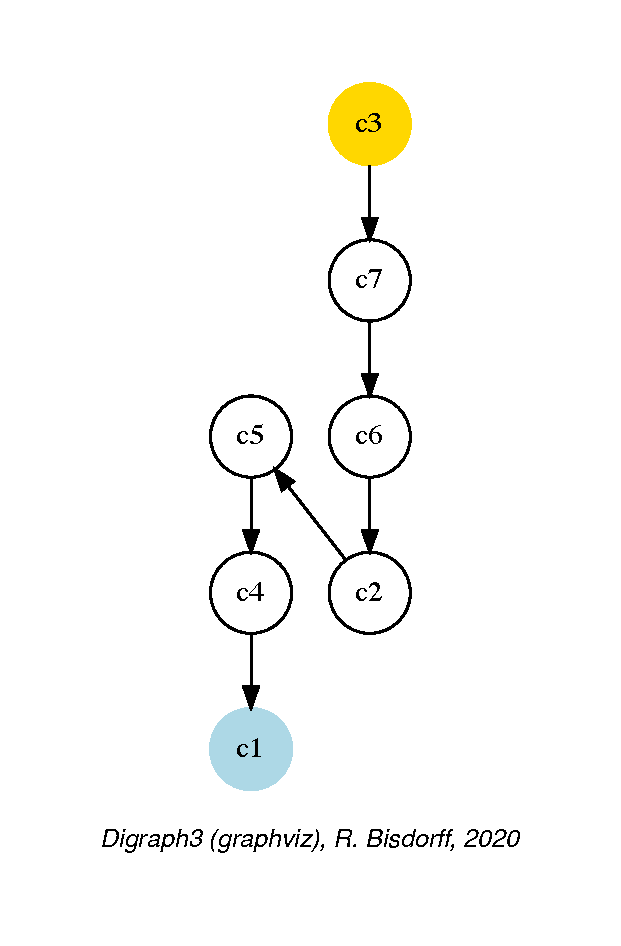
\includegraphics[width=5cm]{Figures/20-2-divGraph.pdf}
\caption{The linear ranking modelled by the majority margins digraph} 
\label{fig:20.2}       % Give a unique label
\end{figure}

\section{Bipolar approval-disapproval voting systems}
\label{sec:20.2}

Traditionally, most of the voting systems in use in the World, do only collect approval votes and abstentions, dismissing potentially strong disapproval opinions, not to be assimilated to voting abstentions. Collecting both explicit approvals ($+1$) and explicit disapprovals ($-1$) essentially enriches the expression of voters' preferences. 

In the \texttt{votingProfiles} module\index{votingProfiles@\texttt{votingProfiles} module} we provide a \texttt{BipolarApprovalVot\-ingProfile} class\index{BipolarApprovalVotingProfile@\texttt{BipolarApprovalVotingProfile} class} for handling voting results where, for each eligible Candidate \texttt{x}, the voters are invited  to \emph{approve} ($+1$), \emph{disapprove} ($-1$), or \emph{ignore} ($0$) the statement that Candidate \texttt{c} should win the election \citep{BAU-2012}.

File \texttt{bpApVotingProfile.py} contains an example of such a approval-disapproval voting profile concerning 100 voters and 15 eligible candidates \footnote{The file \texttt{bpApVotingProfile.py} may be found in the \texttt{examples} directory of the \Digraph resources.}. We can inspect its content with the \texttt{BipolarApprovalVotingProfile} class:\index{BipolarApprovalVotingProfile@\texttt{BipolarApprovalVotingProfile} class}
\begin{lstlisting}[caption={Bipolar approval voting profiles},label=list:20.9]
>>> from votingProfiles import \
...                 BipolarApprovalVotingProfile
>>> bavp = BipolarApprovalVotingProfile('bpApVotingProfile')
>>> bavp
  *------- VotingProfile instance description ------*
    Instance class   : BipolarApprovalVotingProfile
    Instance name    : bpApVotingProfile
    Candidates       : 15
    Voters           : 100
    Attributes       : ['name', 'candidates', 'voters',
                 'approvalBallot', 'netApprovalScores',
                 'ballot']
\end{lstlisting}

Beside the \texttt{candidates} and \texttt{voters} attributes, we discover in Listing~\vref{list:20.10} the \texttt{approvalBallot} attribute which gathers approval-disapproval votes. Its content is the following.
\begin{lstlisting}[caption={Inspecting an approval-disapproval ballot},label=list:20.10]
>>> bavp.approvalBallot
  {'v001':
      {'c01': Decimal('0'),
       ...
       'c04': Decimal('1'), §\label{line:20.10.5}§
       ...
       'c15': Decimal('0')
      },
   'v002':
       {'c01': Decimal('-1'), §\label{line:20.10.10}§
        'c02': Decimal('0'),
        ...
        'c15': Decimal('1')
       },
      ...
   'v100':
     {'c01': Decimal('0'),
      'c02': Decimal('1'),
      ...
      'c15': Decimal('1')
     }
    }
\end{lstlisting}	

Let us denote $A_{\mathtt{v}}$ the set of candidates approved by voter \texttt{v}. In the \texttt{approval\-Ballot} attribute we hence record in fact the bipolar-valued truth characteristic values $r(\mathtt{c} \in A_{\mathtt{v}})$ of the statements that Candidate \texttt{c} \emph{is approved} by voter \texttt{v}. In Listing~\vref{list:20.10} Line~\ref{line:20.10.5}, we observe for instance that voter \texttt{v001} positively approves Candidate \texttt{c04}. And, in Line~\ref{line:20.10.10}, we see that voter \texttt{v002} negatively approves, i.e. positively disapproves Candidate \texttt{c01}.

The \texttt{showApprovalResults()} method\index{showApprovalResults@\texttt{showApprovalResults()}} and the \texttt{showDisapproval\-Re\-sults()} method\index{showDisapprovalResults@\texttt{showDisapprovalResults()}} show how many approvals, respectively disapprovals, each candidate receives.
\begin{lstlisting}
>>> bavp.showApprovalResults()
    Approval results
     Candidate: 'c12' obtains 34 votes §\label{line:avpr.c12}§
     Candidate: 'c05' obtains 30 votes
     Candidate: 'c03' obtains 28 votes
     Candidate: 'c14' obtains 27 votes
     Candidate: 'c11' obtains 27 votes
     Candidate: 'c04' obtains 27 votes
     Candidate: 'c01' obtains 27 votes
     Candidate: 'c13' obtains 24 votes
     Candidate: 'c07' obtains 24 votes
     Candidate: 'c15' obtains 23 votes
     Candidate: 'c02' obtains 23 votes
     Candidate: 'c09' obtains 22 votes
     Candidate: 'c08' obtains 22 votes
     Candidate: 'c10' obtains 21 votes
     Candidate: 'c06' obtains 21 votes
    Total approval votes: 380
    Approval proportion: 380/1500 = 0.25
>>> bavp.showDisapprovalResults()
    Disapproval results
     Candidate: 'c12' obtains 16 votes §\label{line:davpr.c12}§
     Candidate: 'c03' obtains 22 votes
     Candidate: 'c09' obtains 23 votes
     Candidate: 'c04' obtains 24 votes
     Candidate: 'c06' obtains 24 votes
     Candidate: 'c13' obtains 24 votes
     Candidate: 'c11' obtains 25 votes
     Candidate: 'c02' obtains 26 votes
     Candidate: 'c07' obtains 26 votes
     Candidate: 'c08' obtains 26 votes
     Candidate: 'c05' obtains 27 votes
     Candidate: 'c10' obtains 27 votes
     Candidate: 'c14' obtains 27 votes
     Candidate: 'c15' obtains 27 votes
     Candidate: 'c01' obtains 32 votes
    Total disapproval votes: 376
    Disapproval proportion: 376/1500 = 0.25
\end{lstlisting}

In Lines~\ref{line:avpr.c12} and \ref{line:davpr.c12} above, we notice that, of all eligible candidates, it is Candidate \texttt{c12} who receives the highest number of approval votes (34) and the lowest number of disapproval votes (16). Total number of approval, respectively disapproval, votes approaches more or less a proportion of $25\%$ of the $100 \times 15 = 1500$ potential approval votes. About $50\%$ of the latter remain hence ignored. 

When operating now, for each Candidate \texttt{x}, the difference between the number of approval and the number of disapproval votes they receive, we obtain per candidate a corresponding \emph{net approval} score; in fact, the bipolar truth characteristic value of the statement ``\emph{Candidate} \texttt{x} \emph{should win the election}''.
\begin{equation}
r(\text{Candidate x should win the election}) \;=\; \sum_{\mathtt{v}} \big(r(\mathtt{x} \in A_{\mathtt{v}})\big)\;.
\end{equation}

These bipolar characteristic values are stored in the \texttt{netApprovalScores} attribute and may be printed out with the \texttt{showNetApprovalScores()} method\index{showNetApprovalScores@\texttt{showNetApprovalScores()}}:
\begin{lstlisting}
>>> bavp.showNetApprovalScores()
  Net Approval Scores
     Candidate: 'c12' obtains 18 net approvals §\label{line:netapsc:3}§
     Candidate: 'c03' obtains 6 net approvals
     Candidate: 'c05' obtains 3 net approvals
     Candidate: 'c04' obtains 3 net approvals
     Candidate: 'c11' obtains 2 net approvals
     Candidate: 'c14' obtains 0 net approvals
     Candidate: 'c13' obtains 0 net approvals
     Candidate: 'c09' obtains -1 net approvals
     Candidate: 'c07' obtains -2 net approvals
     Candidate: 'c06' obtains -3 net approvals
     Candidate: 'c02' obtains -3 net approvals
     Candidate: 'c15' obtains -4 net approvals
     Candidate: 'c08' obtains -4 net approvals
     Candidate: 'c01' obtains -5 net approvals
     Candidate: 'c10' obtains -6 net approvals
\end{lstlisting}

We observe in Line~\ref{line:netapsc:3} above that Candidate \texttt{c12}, with a net approval score of $34 - 16 = 18$, represents indeed the \emph{best approved} candidate for winning the election. With a net approval score of $28-22 = 6$, Candidate \texttt{c03} appears 2nd-best approved. The net approval scores define hence a potentially weak ranking on the set of eligible election candidates, and the winner(s) of the election is(are) determined by the first-ranked candidate(s).

\section{Pairwise comparison of approval-disapproval votes}
\label{sec:20.3}

The approval votes of each voter define now on the set of eligible candidates three ordered categories: his approved ($+1$), his ignored ($0$) and his disapproved ($-1$) ones. Within each of these three categories we consider the voter's actual preferences as \emph{not communicated}, i.e. as missing data. This gives for each voter a partially determined strict order which we find in the \texttt{ballot} attribute.
\begin{lstlisting}
 >>> bavp.ballot['v001']['c12']
    {'c02': Decimal('1'), 'c11': Decimal('1'),
     'c14': Decimal('1'), 'c04': Decimal('0'),
     'c06': Decimal('1'), 'c05': Decimal('1'),
     'c12': Decimal('0'), 'c13': Decimal('0'),
     'c15': Decimal('1'), 'c01': Decimal('1'),
     'c08': Decimal('1'), 'c07': Decimal('1'),
     'c09': Decimal('0'), 'c03': Decimal('1'),
     'c10': Decimal('0')}
\end{lstlisting}

For voter \texttt{v001}, for instance, the best approved Candidate \texttt{c12} is strictly preferred to Candidates: \texttt{c01}, \texttt{c02}, \texttt{c03}, \texttt{c05}, \texttt{c06}, \texttt{c07}, \texttt{c08}, \texttt{c11}, \texttt{c14} and \texttt{c15}. No candidate is preferred to \texttt{c12} and the comparison with \texttt{c04}, \texttt{c09}, \texttt{c10} and \texttt{c13} is not communicated, hence indeterminate. Mind by the way that the reflexive comparison of \texttt{c12} with itself is, as usual, ignored, i.e. indeterminate. Each voter \texttt{v} defines thus a partially determined transitive strict preference relation denoted $\succ_{\mathtt{v}}$ on the eligible candidates.

For each pair of eligible candidates, we aggregate the previous individual voter's preferences into a truth characteristic of the statement: ``Candidate $x$ is \emph{better approved than} Candidate $y$'', denoted $r(x \succ y)$:
\begin{equation}
  r(x \succ y)\;=\; \sum_{\mathtt{v}} \big(\,r(x \succ_{\mathtt{v}} y)\, \big)\;.
\end{equation}  

We say that Candidate $x$ is \emph{better approved than} Candidate $y$ when $r(x \succ y)\;>\;0$, i.e. there is a majority of voters who approve \emph{more} and disapprove \emph{less} $x$ than $y$. Vice-versa, we say that Candidate $x$ is \emph{not} better approved than Candidate $y$ when $r(x \succ y)\;<\;0$, i.e. there is a majority of voters who disapprove more and approve less $x$ than $y$. This computation is achieved with the \texttt{MajorityMarginsDigraph} constructor.
\begin{lstlisting}
>>> from votingProfiles import MajorityMarginsDigraph
>>> m = MajorityMarginsDigraph(bavp)
>>> m
  *------- Digraph instance description ------*
    Instance class      : MajorityMarginsDigraph
    Instance name       : rel_bpApVotingProfile
    Digraph Order       : 15
    Digraph Size        : 97 §\label{mmdg.8}§
    Valuation domain    : [-100.00;100.00]
    Determinateness (%) : 52.55
    Attributes          : ['name', 'actions',
               'criteria','ballot',
               'valuationdomain', 'relation',
               'order', 'gamma', 'notGamma']
\end{lstlisting}

The resulting digraph \texttt{m} contains 97 positively validated relations (see Line~\ref{mmdg.8} above) and for all pairs $(x,y)$ of eligible candidates, $r(x \succ y)$ takes value in an valuation range from $-100.00$ (unanimously rejected) to $+100.00$ (unanimously approved).

These pairwise $r(x \succ y)$ values can be inspected in a browser view with the \texttt{showHTMLRelationTable()} method: 
\begin{lstlisting}
>>> m.showHTMLRelationTable(relationName='r(x > y)')
\end{lstlisting}
\begin{figure}[ht]
%\sidecaption
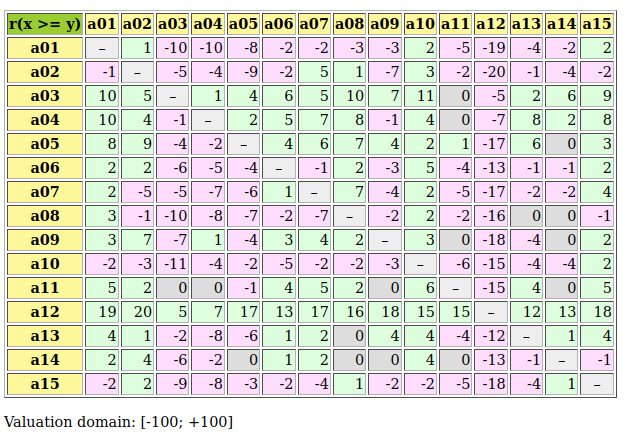
\includegraphics[width=0.8\hsize]{Figures/20-3-majMargAV.png}
\caption{The bipolar-valued pairwise majority margins} 
\label{fig:20.3}       % Give a unique label
\end{figure}

In Fig.~\vref{fig:20.3} it gets apparent that Candidate \texttt{c12} is a \Condorcet winner, i.e. the candidate who beats all the other candidates and, with the given voting profile \texttt{gavp}, should without doubt win the election. This strongly confirms the first-ranked result obtained with the previous net approval scoring. 

Let us eventually compute, with the help of the \NetFlows ranking rule\footnote{See Sect.~\ref{sec:8.3}.}, a linear ranking of the 15 eligible candidates and compare the result with the net approval scores ranking.
\begin{lstlisting}[caption={Comparing the net approval and the \NetFlows rankings},label=list:20.11]
>>> from linearOrders import NetFlowsOrder
>>> nf = NetFlowsOrder(m,Comments=True)
>>> print('NetFlows versus Net Approval Ranking')
>>> print('Candidate\tNetFlows score\tNet Approval score')
>>> for item in nf.netFlows:
...     print( '%9s\t  %+.3f\t %+.1f' %\
...	        (item[1], item[0],\
...              bavp.netApprovalScores[item[1]]) ) 
    NetFlows versus Net Approval Ranking
    Candidate	NetFlows score	Net Approval score
      'c12'	  +410.000	 +18.0
      'c03'	  +142.000	  +6.0
      'c04'	   +98.000	  +3.0
      'c05'	   +54.000	  +3.0
      'c11'	   +34.000	  +2.0
      'c09'	   -16.000	  -1.0 §\label{line:20.11.16}§
      'c14'	   -20.000	  +0.0
      'c13'	   -22.000	  +0.0
      'c06'	   -50.000	  -3.0 §\label{line:20.11.19}§
      'c07'	   -74.000	  -2.0
      'c02'	   -96.000	  -3.0
      'c08'	   -102.000	  -4.0
      'c15'	   -110.000	  -4.0
      'c10'	   -122.000	  -6.0
      'c01'	   -126.000	  -5.0
\end{lstlisting}

In Listing~\vref{list:20.11} we may notice that the \NetFlows rule delivers a ranking that is very similar to the one previously obtained with the corresponding \emph{Net Approval} scores. Only minor inversions do appear, like in the midfield, where Candidate \texttt{c09} advances before Candidates \texttt{c13} and \texttt{c14} (see Line~\ref{line:20.11.16}), and \texttt{c06} and \texttt{c07} swap their positions 9 and 10 (see Line~\ref{line:20.11.19}). The two last-ranked Candidates \texttt{c10} and \texttt{c01} also swap their positions.

This confirms again the pertinence of the net approval scoring approach for finding the winner in an approval-disapproval voting system. Yet, voting by approving ($+1$), disapproving ($-1$) or ignoring ($0$) eligible candidates, may also be seen as a performance evaluation of the eligible candidates on a $\{-1, 0, 1\}$-valued ordinal scale.

\section{Three-valued evaluative voting systems}
\label{sec:20.4}

Following such an epistemic perspective, we may effectively convert the given \texttt{BipolarApprovalVotingProfile} instance into a \texttt{PerformanceTableau} instance, so as to get access to a corresponding outranking decision aiding approach.

Mind that, contrary to the majority margins of the ``\emph{better approved than}'' relation, all voters consider now the approved candidates to be equivalent ($+1$). Same is true for the disapproved ($-1$), respectively the ignored ($0$) candidates. The voter's marginal preferences model this time a complete preorder with three equivalence classes. 

From the saved file \texttt{AVPerfTab.py} (see Line~\ref{line:20.12.1} below), we may construct an outranking relation on the eligible candidates with our standard \texttt{BipolarOutran\-kingDigraph} class constructor. The semantics of this outranking relation are the following:
\begin{itemize}[nosep,leftmargin=0.5cm,rightmargin=0.5cm]
\item We say that Candidate $x$ \emph{outranks} Candidate $y$ when there is a majority of voters who consider $x$ \emph{at least as well evaluated as} $y$;
\item We say that Candidate $x$ is \emph{outranked by} Candidate $y$ when there is a majority of voters who consider $x$ \emph{not at least as well evaluated as} $y$;
\item Otherwise, the outranking situation is indeterminate.
\end{itemize}
\begin{lstlisting}[caption={Computing the outranking digraph},label=list:20.12]
>>> bavp.save2PerfTab(fileName='AVPerfTab',valueDigits=0) §\label{line:20.12.1}§
  *--- Saving as performance tableau in AVPerfTab.py ---*
>>> from outrankingDigraphs import\
...                         BipolarOutrankingDigraph
>>> odg = BipolarOutrankingDigraph('AVPerfTab')
>>> odg
  *------- Object instance description ------*
    Instance class       : BipolarOutrankingDigraph
    Instance name        : rel_AVPerfTab
    Actions              : 15
    Criteria             : 100
    Size                 : 210 §\label{line:20.12.12}§
    Determinateness (%)  : 69.29
    Valuation domain     : [-1.00;1.00]
    Attributes           : ['name', 'actions', 'order,
                       'criteria', 'evaluation', 'NA',
                       'valuationdomain', 'relation',
                       'gamma', 'notGamma', ...]
\end{lstlisting}

The size ($210 = 15 \times 14$) of the resulting outranking digraph \texttt{odg}, shown in Listing~\vref{list:20.12} Line~\ref{line:20.12.12} above, reveals that the corresponding ``\emph{at least as good evaluated as}'' relation models actually a trivial \emph{complete} digraph. All candidates appear to be \emph{equally} at least as well evaluated and the strict ``\emph{better evaluated than}'' (codual) outranking digraph becomes in fact empty. The converted performance tableau does apparently not contain sufficiently discriminatory performance evaluations for supporting any strict preference situations.

Yet, we may nevertheless try to apply again the \NetFlows ranking rule to this complete outranking digraph \texttt{odg} and print side by side the corresponding \NetFlows scores and the previous Net Approval scores. 
\begin{lstlisting}[caption={Comparing the \NetFlows and the Net Approval rankings},label=list:20.13]
>>> from linearOrders import NetFlowsOrder
>>> nf = NetFlowsOrder(odg)
>>> print('NetFlows versus Net Approval Ranking')
>>> print('Candidate\tNetFlows Score\tNet Approval Score')
>>> for item in nf.netFlows:
...     print('%9s\t  %+.3f\t %+.0f' %\
...         (item[1],item[0],\
...          bavp.netApprovalScores[item[1]]) )  
    NetFlows versus Net Approval Ranking
    Candidate    NetFlows score	Net Approval score
      c12	  +4.100	    +18
      c03	  +1.420	     +6
      c04	  +0.980	     +3
      c05	  +0.540             +3
      c11	  +0.340	     +2
      c09	  -0.160	     -1
      c14	  -0.200	      0
      c13	  -0.220	      0
      c06	  -0.500	     -3
      c07	  -0.740	     -2
      c02	  -0.960	     -3
      c08	  -1.020	     -4
      c15	  -1.100	     -4
      c10	  -1.220	     -6
      c01	  -1.260	     -5
\end{lstlisting}

Despite its apparent poor strict preference discriminating power, we obtain in Listing~\vref{list:20.13} here \NetFlows scores that are directly proportional (divided by $100$) to the scores obtained with the \emph{better approved than} majority margins digraph \texttt{m} (see List.~\vref{list:20.11}).

Encouraged by this positive result, we may furthermore compute a \Rubis best choice recommendation (see Chap.~\ref{sec:4}).
\begin{lstlisting}[caption={Computing a best social choice recommendation},label=list:20.14]
>>> odg.showBestChoiceRecommendation()
  Rubis best choice recommendation(s) (BCR)
   (in decreasing order of determinateness)   
   Credibility domain: [-1.00,1.00]
  === >> ambiguous first choice(s) 
   * choice        : ['c01','c02','c03','c04','c05', §\label{line:20.14.6}§
                      'c06','c07','c08','c09','c10',
                      'c11','c12','c13','c14','c15'] §\label{line:20.14.8}§
    independence   : 0.06
    dominance      : 1.00
    absorbency     : 1.00
    covering (%)   : 100.00
    determinateness (%) : 61.13
    - most credible action(s) = {
        'c12': 0.44, 'c03': 0.34, 'c04': 0.30, §\label{line:20.14.15}§
        'c14': 0.28, 'c13': 0.24, 'c06': 0.24,
        'c11': 0.20, 'c10': 0.20, 'c07': 0.20,
        'c01': 0.20, 'c08': 0.18, 'c05': 0.18,
        'c15': 0.14, 'c09': 0.14, 'c02': 0.06, }
   === >> ambiguous last choice(s)
    * choice        : ['c01','c02','c03','c04','c05',
                      'c06','c07','c08','c09','c10',
                      'c11','c12','c13','c14','c15']
     independence   : 0.06
     dominance      : 1.00
     absorbency     : 1.00
     covered (%)    : 100.00
     determinateness (%) : 63.73
     - most credible action(s) = {
         'c13': 0.36, 'c06': 0.36, 'c15': 0.34, §\label{line:20.14.30}§
         'c01': 0.34, 'c08': 0.32, 'c07': 0.30,
         'c02': 0.30, 'c14': 0.28, 'c11': 0.28,
         'c09': 0.28, 'c04': 0.26, 'c10': 0.24,
         'c05': 0.20, 'c03': 0.20, 'c12': 0.06, }
\end{lstlisting}

The strict outranking digraph $(\sim (-odg))$ being actually $empty$, we obtain a unique \emph{ambiguous} --first as well as last-- choice recommendation which trivially retains all fifteen candidates (see List.~\vref{list:20.14} Lines~\ref{line:20.14.6}-\ref{line:20.14.8} above). Yet, the bipolar-valued best choice membership characteristic vector reveals that, among all the fifteen potential winners, it is indeed Candidate \texttt{c12} the most credible one with a $72\%$ majority of voters' support (see Line~\ref{line:20.14.15}, $(0.44 + 1.0)/2\;=\; 0.72$); followed by Candidate \texttt{c03} ($67\%$) and Candidate \texttt{c04} ($65\%$). Similarly, Candidates \texttt{c13} and \texttt{c06} represent the most credible losers with a $68\%$ majority voters' support (Line~\ref{line:20.14.30}).

We observe here empirically that \emph{evaluative} voting systems, using three-valued ordinal performance scales, match closely corresponding approval-disapproval voting systems. The latter systems model, however, more faithfully the very preferential information that is expressed with \emph{approved}, \emph{disapproved} and \emph{ignored} statements. The corresponding evaluation on a three-level scale, being value (numbers) based, cannot express the fact that in approval-disapproval voting system there is no preferential information given concerning the pairwise comparison of all approved, respectively disapproved or ignored candidates.

Let us finally illustrate how approval-disapproval voting systems may favour multipartisan supported candidates. We shall therefore compare \emph{approval-disapproval} versus \emph{uninominal plurality} election results when considering a highly divisive and partisan political context.
 
\section{Favouring multipartisan candidates}
\label{sec:20.5}

In modern democracy, politics  are largely structured by political parties and activists. Let us so consider an approval-disapproval voting profile \texttt{dvp} where the random voter behaviour is simulated from two pre-electoral polls concerning a political scene with essentially two major highly competing parties, like the one existing in the US.
\begin{lstlisting}[caption={A random approval-disapproval voting profile in a divisive political context},label=list:20.15]
>>> dvp = RandomBipolarApprovalVotingProfile(\
...                numberOfCandidates=15,\
...                numberOfVoters=100,
...                approvalProbability=0.25,
...                disapprovalProbability=0.25,
...                WithPolls=True,
...                partyRepartition=0.5,
...                other=0.05,
...                DivisivePolitics=True,
...                seed=200)
>>> dvp.showRandomPolls()
  Random repartition of voters
  Party-1 supporters : 45 (45.00%)
  Party-2 supporters : 49 (49.00%)
  Other voters       : 6 (06.00%)
  *---------------- random polls -----------------
  Party-1(45.0%) | Party-2(49.0%) |   expected  
  ------------------------------------------------
  'c05' : 24.10% | 'c07' : 24.10% | 'c07' : 11.87%
  'c14' : 23.48% | 'c10' : 23.48% | 'c10' : 11.60%
  'c03' : 15.13% | 'c01' : 15.13% | 'c05' : 10.91%
  'c12' : 07.55% | 'c04' : 07.55% | 'c14' : 10.67%
  'c08' : 07.11% | 'c09' : 07.11% | 'c01' : 07.67%
  'c15' : 04.37% | 'c13' : 04.37% | 'c03' : 07.09%
  'c11' : 03.99% | 'c02' : 03.99% | 'c04' : 04.55%
  'c06' : 03.80% | 'c06' : 03.80% | 'c09' : 04.49%
  'c02' : 02.79% | 'c11' : 02.79% | 'c12' : 04.32%
  'c13' : 02.63% | 'c15' : 02.63% | 'c08' : 04.30%
  'c09' : 02.24% | 'c08' : 02.24% | 'c06' : 03.57%
  'c04' : 01.89% | 'c12' : 01.89% | 'c13' : 03.32%
  'c01' : 00.57% | 'c03' : 00.57% | 'c15' : 03.25%
  'c10' : 00.20% | 'c14' : 00.20% | 'c02' : 03.21%
  'c07' : 00.14% | 'c05' : 00.14% | 'c11' : 03.16%
\end{lstlisting}   

In Listing~\vref{list:20.15}, the divisive political situation is reflected by the fact that Party-1 and Party-2 supporters show strict opposite preferences. The leading candidates of Party-1 (\texttt{c05} and \texttt{c14}) are last choices for Party-2 supporters and, Candidates \texttt{c07} and \texttt{c10}, leading candidates for Party-2 supporters, are similarly the least choices for Party-1 supporters.

No clear winner may be guessed from these pre-election polls. As Party-2 shows however slightly more supporters than Party-1, the expected winner in an uninominal plurality or instant-run-off voting system will be Candidate \texttt{c07}, i,e, the leading candidate of majority Party-2 (see below).
\begin{lstlisting}
>>> dvp.computeSimpleMajorityWinner()
  ['c07']
>>> dvp.computeInstantRunoffWinner()
  ['c07']
\end{lstlisting}

Now, in a corresponding approval-disapproval voting system, Party-1 supporters will usually approve their leading candidates and disapprove the leading candidates of Party-2. Vice versa, Party-2 supporters will usually approve their leading candidates and disapprove the leading candidates of Party-1. Let us consult the resulting approval votes per candidate.
\begin{lstlisting}
>>> dvp.showApprovalResults()
     Candidate: 'c07' obtains 30 votes
     Candidate: 'c10' obtains 28 votes
     Candidate: 'c05' obtains 28 votes
     Candidate: 'c01' obtains 28 votes
     Candidate: 'c03' obtains 26 votes
     Candidate: 'c02' obtains 26 votes
     Candidate: 'c12' obtains 25 votes
     Candidate: 'c14' obtains 24 votes
     Candidate: 'c13' obtains 24 votes
     Candidate: 'c09' obtains 21 votes
     Candidate: 'c04' obtains 21 votes
     Candidate: 'c08' obtains 19 votes
     Candidate: 'c06' obtains 17 votes
     Candidate: 'c15' obtains 15 votes
     Candidate: 'c11' obtains 12 votes
    Total approval votes: 344
    Approval proportion: 344/1500 = 0.23
\end{lstlisting}

When considering only the approval votes, we find confirmed above that the leading candidate of Party-2 obtains in this simulation a plurality of approval votes. In uninominal plurality or instant-runoff voting systems, this candidate wins hence the election, quite to the despair of Party-1 supporters. As a foreseeable consequence, this election result will be more or less aggressively contested which leads to a loss of popular trust in democratic elections and institutions.

If we look however on the corresponding disapprovals, we discover that, not surprisingly, the leading candidates of both parties collect by far the highest number of disapproval votes. 
\begin{lstlisting}
>>> dvp.showDisapprovalResults()
     Candidate: 'c02' obtains 14 votes
     Candidate: 'c04' obtains 14 votes
     Candidate: 'c13' obtains 14 votes
     Candidate: 'c06' obtains 15 votes
     Candidate: 'c09' obtains 15 votes
     Candidate: 'c08' obtains 16 votes
     Candidate: 'c11' obtains 16 votes
     Candidate: 'c15' obtains 18 votes
     Candidate: 'c12' obtains 20 votes
     Candidate: 'c01' obtains 29 votes
     Candidate: 'c03' obtains 30 votes
     Candidate: 'c10' obtains 37 votes
     Candidate: 'c07' obtains 44 votes
     Candidate: 'c14' obtains 45 votes
     Candidate: 'c05' obtains 49 votes
    Total disapproval votes: 376
    Disapproval proportion: 376/1500 = 0.25
\end{lstlisting}

Balancing now approval against disapproval votes will favour the moderate, bipartisan supported, candidates.
\begin{lstlisting}
>>> dvp.showNetApprovalScores()
    Net Approval Scores
     Candidate: 'c02' obtains 12 net approvals
     Candidate: 'c13' obtains 10 net approvals
     Candidate: 'c04' obtains 7 net approvals
     Candidate: 'c09' obtains 6 net approvals
     Candidate: 'c12' obtains 5 net approvals
     Candidate: 'c08' obtains 3 net approvals
     Candidate: 'c06' obtains 2 net approvals
     Candidate: 'c01' obtains -1 net approvals
     Candidate: 'c15' obtains -3 net approvals
     Candidate: 'c11' obtains -4 net approvals
     Candidate: 'c03' obtains -4 net approvals
     Candidate: 'c10' obtains -9 net approvals
     Candidate: 'c07' obtains -14 net approvals
     Candidate: 'c14' obtains -21 net approvals
     Candidate: 'c05' obtains -21 net approvals
\end{lstlisting}

Candidate \texttt{c02}, appearing in the pre-electoral polls in the midfield (in position 7 for Party-2 and in position 9 for Party-1 supporters, see List.\vref{list:20.15}), shows indeed the highest net approval score. Second highest net approval score obtains Candidate \texttt{c13}, in  position 6 for Party-2 and in position 10 for Party-1 supporters.

Figure~\vref{fig:20.4}, showing the \NetFlows ranked relation table of the ``\emph{better approved than}'' majority margins digraph, confirms below this net approval scoring result.
\begin{lstlisting}
>>> m = MajorityMarginsDigraph(dvp)
>>> m.showHTMLRelationTable(\
...      actionsList=m.computeNetFlowsRanking(),
...      relationName='r(x > y)')
\end{lstlisting}	   
\begin{figure}[ht]
%\sidecaption
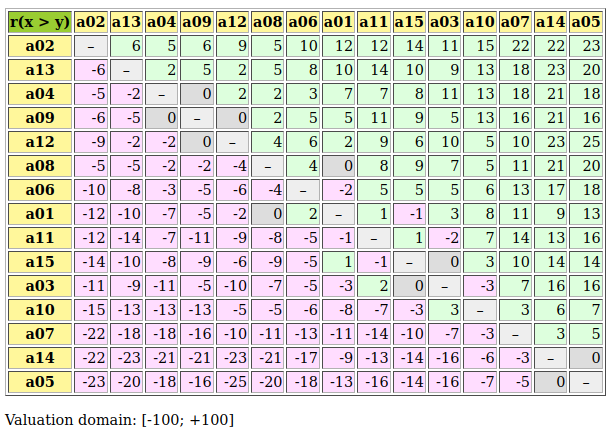
\includegraphics[width=0.8\hsize]{Figures/20-4-majMargDAV.png}
\caption{The pairwise \emph{better approved than} majority margins} 
\label{fig:20.4}       % Give a unique label
\end{figure}

Candidate \texttt{c02} appears indeed \emph{better approved than} any other candidate (\Condorcet winner); and, the leading Candidates of Party-1, \texttt{c05} and \texttt{c14}, are \emph{less approved than} any other candidates (weak \Condorcet losers).
\begin{lstlisting}
>>> m.computeCondorcetWinners()
  ['c02']
>>> m.computeWeakCondorcetLosers()
  ['c05','c14']
\end{lstlisting}

We see this result furthermore confirmed when computing the corresponding first, respectively last choice recommendation.    
\begin{lstlisting}
>>> m.showBestChoiceRecommendation()
  Rubis best choice recommendation(s) (BCR)
   (in decreasing order of determinateness)   
   Credibility domain: [-100.00,100.00]
   === >> potential first choice(s)
    * choice              : ['c02']
      independence        : 100.00
      dominance           : 5.00
      absorbency          : -23.00
      covering (%)        : 100.00
      determinateness (%) : 52.50
      - most credible action(s) = { 'c02': 5.00, }
   === >> potential last choice(s) 
    * choice              : ['c05', 'c14']
      independence        : 0.00
      dominance           : -23.00
      absorbency          : 5.00
      covered (%)         : 100.00
      determinateness (%) : 50.00
      - most credible action(s) = { }
\end{lstlisting}

Candidate \texttt{c02}, being actually a \Condorcet winner, gives an initial prekernel of digraph \texttt{m}, whereas Party-1 leading Candidates \texttt{c05} and \texttt{c14}, both being weak \Condorcet losers, give together a terminal prekernel. They hence represent our \emph{first choice}, respectively, \emph{last choice} recommendations for winning this simulated election.

It is worthwhile noticing again the essential structural and computational role, the ignored value is playing in approval-disapproval voting systems. This epistemic and logical \emph{neutral} term is needed indeed for handling in a consistent and efficient manner \emph{not communicated votes} and/or \emph{indeterminate} preferential statements.

Let us conclude by predicting that, for leading political candidates in an aggressively divisive political context, the perspective to easily fail election withan approval-disapproval voting system, might or will induce a change in the usual way of running electoral campaigns. Political parties and politicians, who avoid aggressive competitive propaganda and instead propose multipartisan collaborative social choices, will be rewarded with better election results than any kind of extremism. It could mean the end of sterile political obstructions and war like electoral battles. \emph{Let's do it !}.

\vspace{\baselineskip}
The last Part V of this monograph illustrates in three chapters computational resources for working with simple undirected graphs.

%%%%%%% The chapter bibliography
%\normallatexbib
%\clearpage
%\phantomsection
%\addcontentsline{toc}{section}{Chapter Bibliography}
\input{Bibliographies/20-chapterTemperingPlurality.bbl}
%\bibliographystyle{spbasic}
%\bibliography{03-backMatters/reference}

%\bibliographystyle{spbasic}
%\bibliography{03-backMatters/reference}

%\bibliographystyle{spbasic}
%\bibliography{03-backMatters/reference}

%\bibliographystyle{spbasic}
%\bibliography{03-backMatters/reference}
